% This is the root file of the thesis: thesis.tex

%%===================================
\documentclass[12pt, twoside]{report}

\usepackage{url}
\usepackage{amsmath}
\usepackage[utf8]{inputenc} % This defines the font-encoding you prefer to use
\usepackage[pdftex]{graphicx}
\usepackage[bindingoffset=1cm,centering,includeheadfoot,margin=2cm]{geometry}
\usepackage{csquotes}
\usepackage{placeins}
\usepackage{float}
\usepackage[
    citestyle=numeric-comp,
    backend=biber,
    bibencoding=inputenc
    ]{biblatex}
\addbibresource{refs.bib}
\usepackage[toc,page]{appendix}
\usepackage{setspace}
\linespread{1.5}
\setcounter{tocdepth}{2} 
\usepackage[colorlinks=true, pdfstartview=FitV,
linkcolor=blue, citecolor=blue, urlcolor=blue]{hyperref}
\setlength{\parindent}{0pt} % No indentation between paragraphs
\setlength{\parskip}{10pt} % Space between paragraphs

% Tables
\usepackage{ltxtable}
\usepackage{booktabs}

% Needed for code listings
\usepackage{listings}
% https://tex.stackexchange.com/questions/106770/how-to-add-line-numbers-to-a-program-listing-code
\usepackage{color}

% Subfigure
\usepackage{subcaption}

\usepackage{floatpag} % to move floatpagenr to topright

% Fußnote
\usepackage[hang]{footmisc}
\setlength{\footnotemargin}{-0.8em}

\usepackage{csquotes}
\usepackage{afterpage} % needed for empty page after front

%%===================================
% Custom definitions
    
% Signal color
\definecolor{signalColor}{RGB}{164, 63, 114}
\newcommand\signal[1]{\textbf{\textcolor{signalColor}{#1}}}
    
% List with less space between items
\newenvironment{cList}{
\begin{itemize}
  \setlength{\itemsep}{0pt}
  \setlength{\parskip}{0pt}
  \setlength{\parsep}{0pt}
}{\end{itemize}}

% Enumeration with less space between items
\newenvironment{cEnum}{
\begin{enumerate}
  \setlength{\itemsep}{0pt}
  \setlength{\parskip}{0pt}
  \setlength{\parsep}{0pt}
}{\end{enumerate}}

% Space LoL
\let\Chapter\chapter
\def\chapter{\addtocontents{lol}{\protect\addvspace{10pt}}\Chapter}

% Code definition JSON
\definecolor{numberColor}{RGB}{24,118,129}
\newcommand\JSONnumbervaluestyle{\color{numberColor}}
\newcommand\JSONstringvaluestyle{\color{signalColor}}

\newif\ifcolonfoundonthisline

\makeatletter

\lstdefinestyle{json}{
  showstringspaces    = false,
  keywords            = {false,true},
  alsoletter          = 0123456789.,
  morestring          = [s]{"}{"},
  stringstyle         = \ifcolonfoundonthisline\JSONstringvaluestyle\fi,
  MoreSelectCharTable =%
    \lst@DefSaveDef{`:}\colon@json{\processColon@json},
  basicstyle          = \ttfamily,
  keywordstyle        = \ttfamily\bfseries
}

\lstset{
  numbers=left,
  lineskip={-1.5pt},
  captionpos=b,
  basicstyle=\footnotesize\ttfamily,
  xleftmargin=1cm,
  breaklines=true
}

\newcommand\processColon@json{%
  \colon@json%
  \ifnum\lst@mode=\lst@Pmode%
    \global\colonfoundonthislinetrue%
  \fi
}

\lst@AddToHook{Output}{%
  \ifcolonfoundonthisline%
    \ifnum\lst@mode=\lst@Pmode%
      \def\lst@thestyle{\JSONnumbervaluestyle}%
    \fi
  \fi
  \lsthk@DetectKeywords% 
}

\lst@AddToHook{EOL}%
  {\global\colonfoundonthislinefalse}

\makeatother
% End code definition JSON

% Rename listings and toc
\renewcommand{\contentsname}{Table of Contents}
\renewcommand{\lstlistlistingname}{List of Listings}

%=====================
\newcommand{\HRule}[1]{\rule{\linewidth}{#1}} 	% Horizontal rule

\makeatletter							% Title
\def\printtitle{%						
    {\centering \@title\par}}
\makeatother									

\makeatletter							% Author
\def\printauthor{%					
    {\centering \large \@author}}				
\makeatother	

% Metadata (Change this)
% --------------------------------------------------------------------
\title{	\normalsize \textsc{Technische Universität Berlin} 	% Subtitle
		 	\\[2.0cm]								% 2cm spacing
			\HRule{0.5pt} \\						% Upper rule
			\LARGE \textbf{\uppercase{FOG computing project report}}	% Title
			\HRule{2pt} \\ [0.5cm]		% Lower rule + 0.5cm spacing
			\normalsize \today			% Todays date
		}

\author{
		Jacek Janczura, Marina Mursa, Clemens Peters,\\ Nursultan Shabykeev, Ali Karaki, Marius Schidlack, Alexandre Rozier \\ 
}

\usepackage{enumitem}

\begin{document}

% Maketitle
% ------------------------------------------------------------------------------
\thispagestyle{empty}		% Remove page numbering on this page

\printtitle					% Print the title data as defined above
  	\vfill
\printauthor				% Print the author data as defined above
\newpage

%%========================================
% Frontmatter

\include{frontmatter/front} % This is the titlepage
\setcounter{page}{0}
\pagenumbering{Roman}
\include{frontmatter/summary}
\tableofcontents

\clearpage
\phantomsection
\addcontentsline{toc}{section}{\listfigurename}
\listoffigures

\clearpage
\phantomsection
\addcontentsline{toc}{section}{\lstlistlistingname}
\lstlistoflistings

%%=========================================
% Mainmatter

\cleardoublepage
\setcounter{page}{0}
\pagenumbering{arabic}
\include{mainmatter/01_introduction}
% Include more chapters as required.
\chapter{Introduction - Marina}
    This chapter gives a brief introduction to the content of the project through presenting the motivation behind it, and statement of the goals.
    \section{Motivation}
In a world hooked on technologies, a connection to the outside world is crucial, even when a person is in the car. This is the reason behind every car manufacturer trying to come up with some technological ecosystem that won’t just connect the car, but also the user to the world around him.
BMW technology package called ConnectedDrive has currently over 8 million cars that connect daily to almost 300 micro services that guarantee not only entertainment but most importantly the security of the users. This services range from Map Updates to Real Time Traffic Information to Concierge Services. Due to such a diversified range with high utility for the user, the cars become moving data centers.
Aggregating these connections by time, one type of data that results is represented in the form of requests to connect to BMW servers (to get access the the mentioned services)  per second (requests/sec)\footnote{https://www.bmw-connecteddrive.de/app/index.html\#/portal/store}. 
Having such huge amounts of data generated continuously, a daily pattern can be observed that corresponds to the intuitive rush-hour peaks.
\begin{figure}[h]
    \centering
    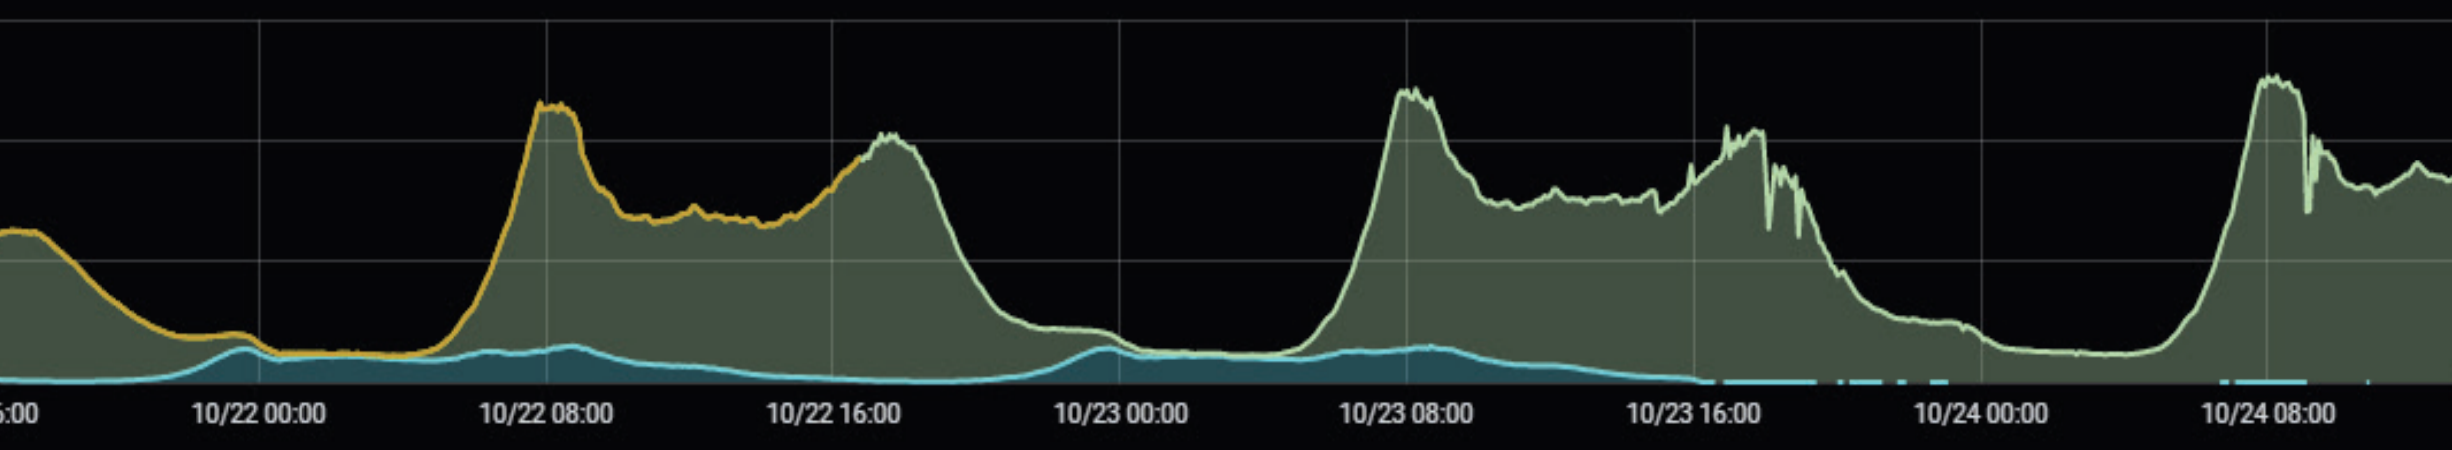
\includegraphics[width=1\textwidth]{images/data-graph.png}
    \caption{Visualisation of BMW data in form of requests per second }
\end{figure}

    \section{Goals}
The primary goal of this project is to develop a framework, based on AWS service, that would be able to detect in a real-time environment a deviation from the pattern mentioned above, label it as an anomaly, and escalate a notification to a tool, e.g. a Slack channel, in the form of an alert accompanied by a small visual representation of the problem.\\
As a secondary challenge, the project attempts to incorporate a prediction feature, that would deliver information which would allow for predictive scaling of the infrastructure based on a generated short-term prognosis. The purpose of this feature has a deeply financial reasoning behind, allowing the team to adapt the infrastructure besed on the predicted needs, thus reducing the expenses with the AWS services. \\
The final goal of the project was to come up with an additional set of recommendations and potential improvements to the delivered product.  This list of future features that can be investigated by the BMW team in order to assess the prospective value of adding them to their existing framework.
\chapter{System architecture - Jacek}
    % Marius: I think this part should establish a little more on the motivation and introduction part. Right now I think the reader has no idea what this is about if they were never exposed to the project before.

We assumed that we might not have an access to the real time data and the only data that will be provided to us might be a batch data. For that reason and to be able to work in parallel the system architecture in our project is composed of 2 approaches: \textbf{fixed} and \textbf{stream}. \\
In the fixed approach we will train and test multiple machine learning models, not to wait for whole real time infrastructure.
In stream approach we will create the whole streaming infrastructure and than reuse already prepared, trained and tested models from the fixed approach.\\
At the end we received the following system architecture fig. \ref{fig:architecture}. In the final architecture we are using previously gathered data(fixed) to train the ML models. Those trained models will be used for a real time streamed data in which we will try to detect anomalies.  

\subsection{Brief, high level description of the system architecture - Jacek}
\begin{itemize}
\item \textbf{In a fixed approach} we use fixed chunks of data provided by BMW to train the models deployed in AWS SageMaker. 
\item \textbf{In a stream approach} we assumed that the data might come from multiple sources. We gather these data using Kinesis Stream as a queue. Then using a Amazon Simple Notification Service (SNS) lambdas is triggered. This lambdas feed the models with incoming data. In case of anomaly detection feeding lambda is triggering different notification functions using SNS topic to inform user that anomaly has been detected.
\end{itemize}
% Marius: Whats a lambda? Whats SNS?

A more detailed description is provided in a following chapter.
\begin{figure}[h]
    \centering
    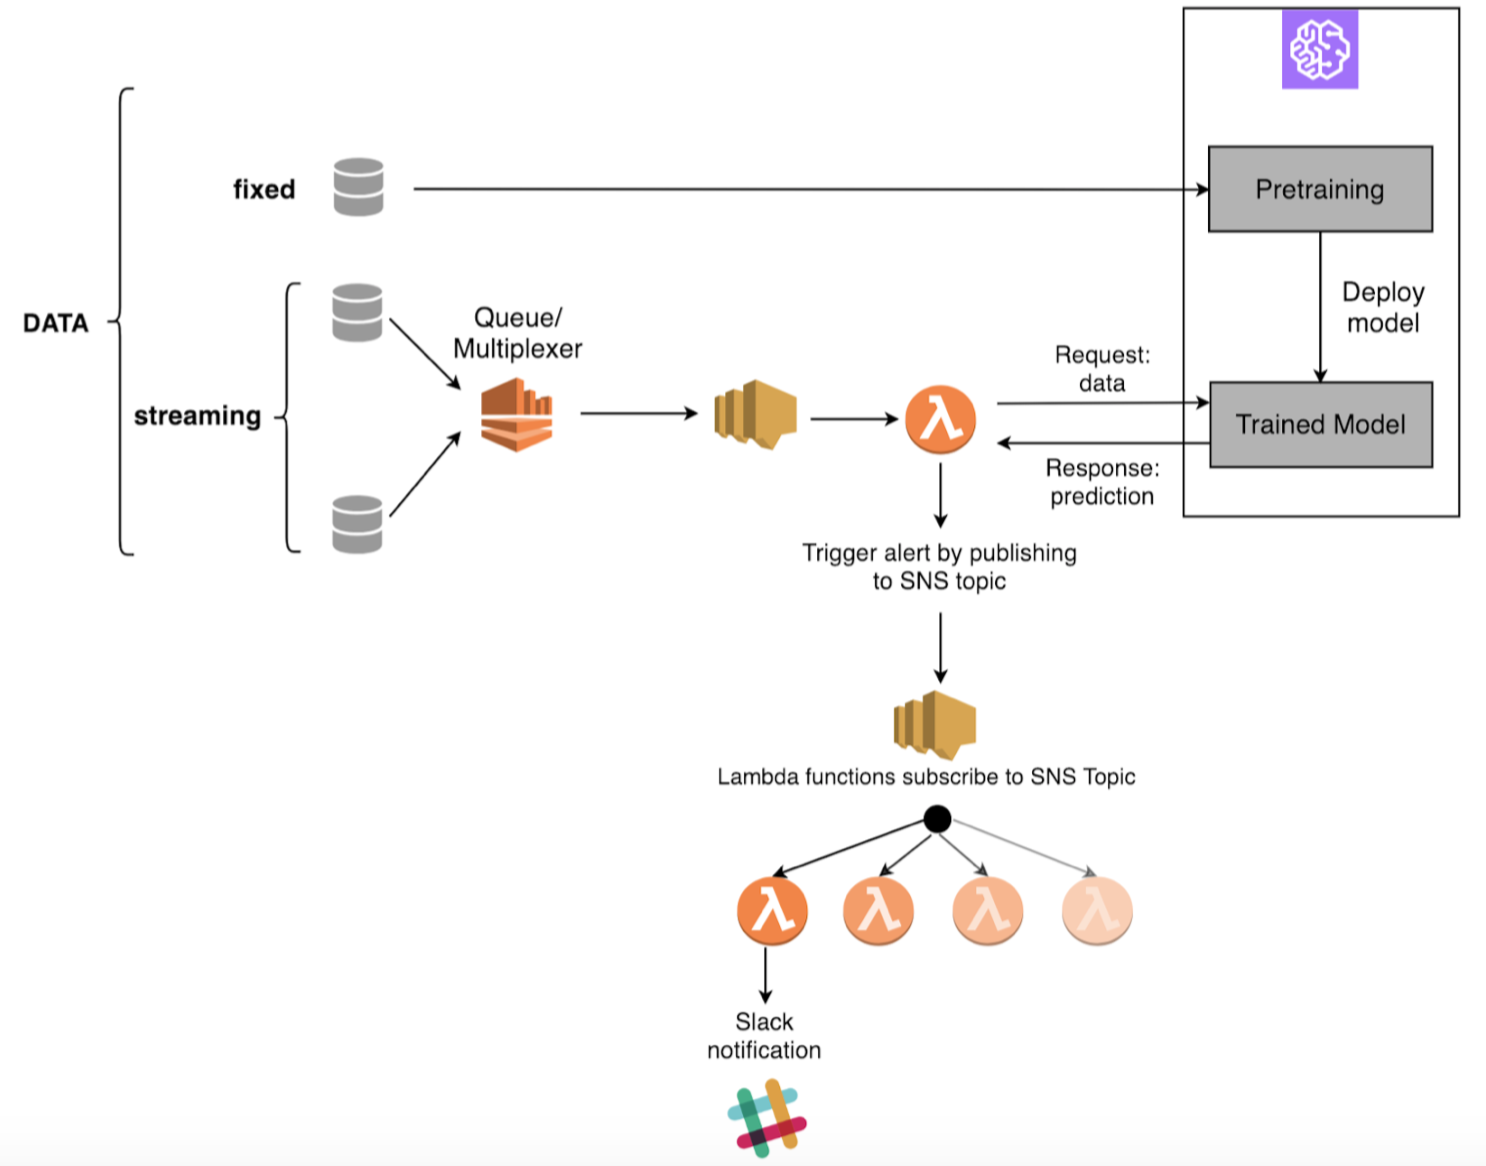
\includegraphics[width=0.8\textwidth]{images/sys-architecture.png}
    \caption{System architecture schema}
    \label{fig:architecture}
\end{figure}
    

       This chapter will give an overview to the ways this project was managed internally, as well as by the supervisors. It includes a detailed introduction to the Kanban - management tool, followed by complementary techniques used by the team to further improve the working process.
    \section{Kanban}
For internal management of the team, based on the suggestions of our industry partners, it was decided to use an Agile product management technique - Kanban. It emphasizes on a continuous delivery mindset, trying not to overburden the development team. Like other Agile techniques, it was designed to facilitate communication and division of work inside the team, while giving live updates so each member can keep up with the process. The simple and intuitive structure helps the team work in a more efficient way.
% Marius: More efficient than what?
        \subsection{Principles}
        Kanban is build by respecting the following 3 principles:
            \begin{enumerate}
  \item \textbf{Visualization}: Kanban uses mechanisms organised in a Kanban board. The board, by presenting all the tasks at once, in an easy to grasp manner, gives the developer a better understanding of the context, thus facilitating the workflow.
  \item \textbf{Limited amount of work}: because the number of tasks are limited from a week to another (as well as the number of cards stored in production) the team does not feel overburdened with work, and is not pressured to deliver something by sacrificing on the quality aspect.
  \item \textbf{Continuous flow}: when a member is done with his/her tasks, he/she can just move forward with the work process by picking up the next tasks (placed on the top of the stack). This way nobody sits around waiting to be designated with work, thus ensuring a continuous workflow.
\end{enumerate}
        \subsection{Benefits}
        Taking in consideration the above mentioned information, it is easy to identify the way this project management method can improve the delivery process of a product, following are a couple of its advantages: 
            \begin{enumerate}
                \item \textit{Kanban methodology utilizes short working cycles.} In the case of this project the cycle was limited at one week (with an exception during the winter break).  This 1 week cycles ensured a continuous delivery process, where the industry partners had the opportunity to keep the team in check, by introducing new features/corrections in the process.
                \item \textit{Kanban is very responsive to change and feedback.} As mentioned above, thanks to a short cycle, the BMW representatives had the opportunity to introduce change in an utile time, by coming up with new features or scenarios, as well as feedback to improve or correct the direction of the project.
                \item \textit{Kanban removes time wasting activities.} While popular management techniques require a series of mandatory daily meetings and discussions, Kanban eliminates this type of time wasting activities. Meetings were organized once a week or on team’s request, in cases of confusion or identification of impediments of the working process that should be discussed and solved at team level.
            \end{enumerate}
        \subsection{Roles}
Given the Kanban approach, it does not have well predefined roles. It suggests to start from the structure of your team, and current management, and to evolve it as seen necessary, taken in consideration the specific of the methodology.
As the team had no previous experience working together, it decided to have a Project Manager that would facilitate the communication between them and the supervisors, as well as take care of organizational issues.
The project manager’s responsibilities are:
            \begin{itemize}
              \item Managing the Kanban board (in Trello) which means writing down the tasks, assigning responsible people, adding labels, deadlines (if necessary), updating the progress, and cleaning up the board by periodically archiving the old cards.
              \item Managing other means of communication, like Slack, by organizing specific channels, setting up notifications and reminders.
              \item Setting up and managing meetings, making sure they are productive and that the team is up to date with project’s progress.
              \item Being the spokesperson for the team, mediating the communication with the supervisors.
            \end{itemize}
        \subsection{Kanban board}
As already mentioned above, Kanban uses a board as it’s main management tool. A Kanban board is designed to help visualise the workflow. A typical board can be broken down into the following elements:
            \begin{enumerate}
                \item Cards or Visual Signals 
                \item Columns
                \item Work in Progress (WIP) Limits
            \end{enumerate}
The visual signals are usually the tasks that are written on stickies, in the case of a physical board, or on cards, in the case of software based boards. Each card encapsulates one user story, and all the user stories should require an equal or at least close enough effort. Once written down and attached to the board, these visual signals help the team, as well as other stakeholders, understand the product development.
Columns represent different production stages that an user story can be in. All these stages together compose the workflow. The columns can be as simple as “To do”, “In progress” and “Done”, to more complicated stages, depending on the complexity of the development process.
Work in Progress Limits are the maximum number of cards that can be placed in a certain column at a certain period of time. This is done in order to limit the team’s ability to commit to too much work in a short period of time.
                \subsubsection{Trello as a Kanban board}
For the project, the team decided, following the supervisors’ suggestion, to use a digital board. This allows it not to share a physical space (like an office), and to work remotely and asynchronously. Trello is one of the simplest and easiest way to mimic a Kanban board by allowing the users to create lists, that mimic the columns, and cards that represent user stories.

For this project, it was decided to create the following workflow structure:
    \begin{itemize}
        \item Backlog - aggregates all user stories
        \item Breakdown (Doing and Done)- splits up user stories in smaller units of work
        \item Implementation (Doing and Done) - indicates what cards are currently in work
        \item Validation (Doing and Done)- tests the finished user stories against the definition-of-done.
    \end{itemize}

    \begin{figure}[h]
        \centering
        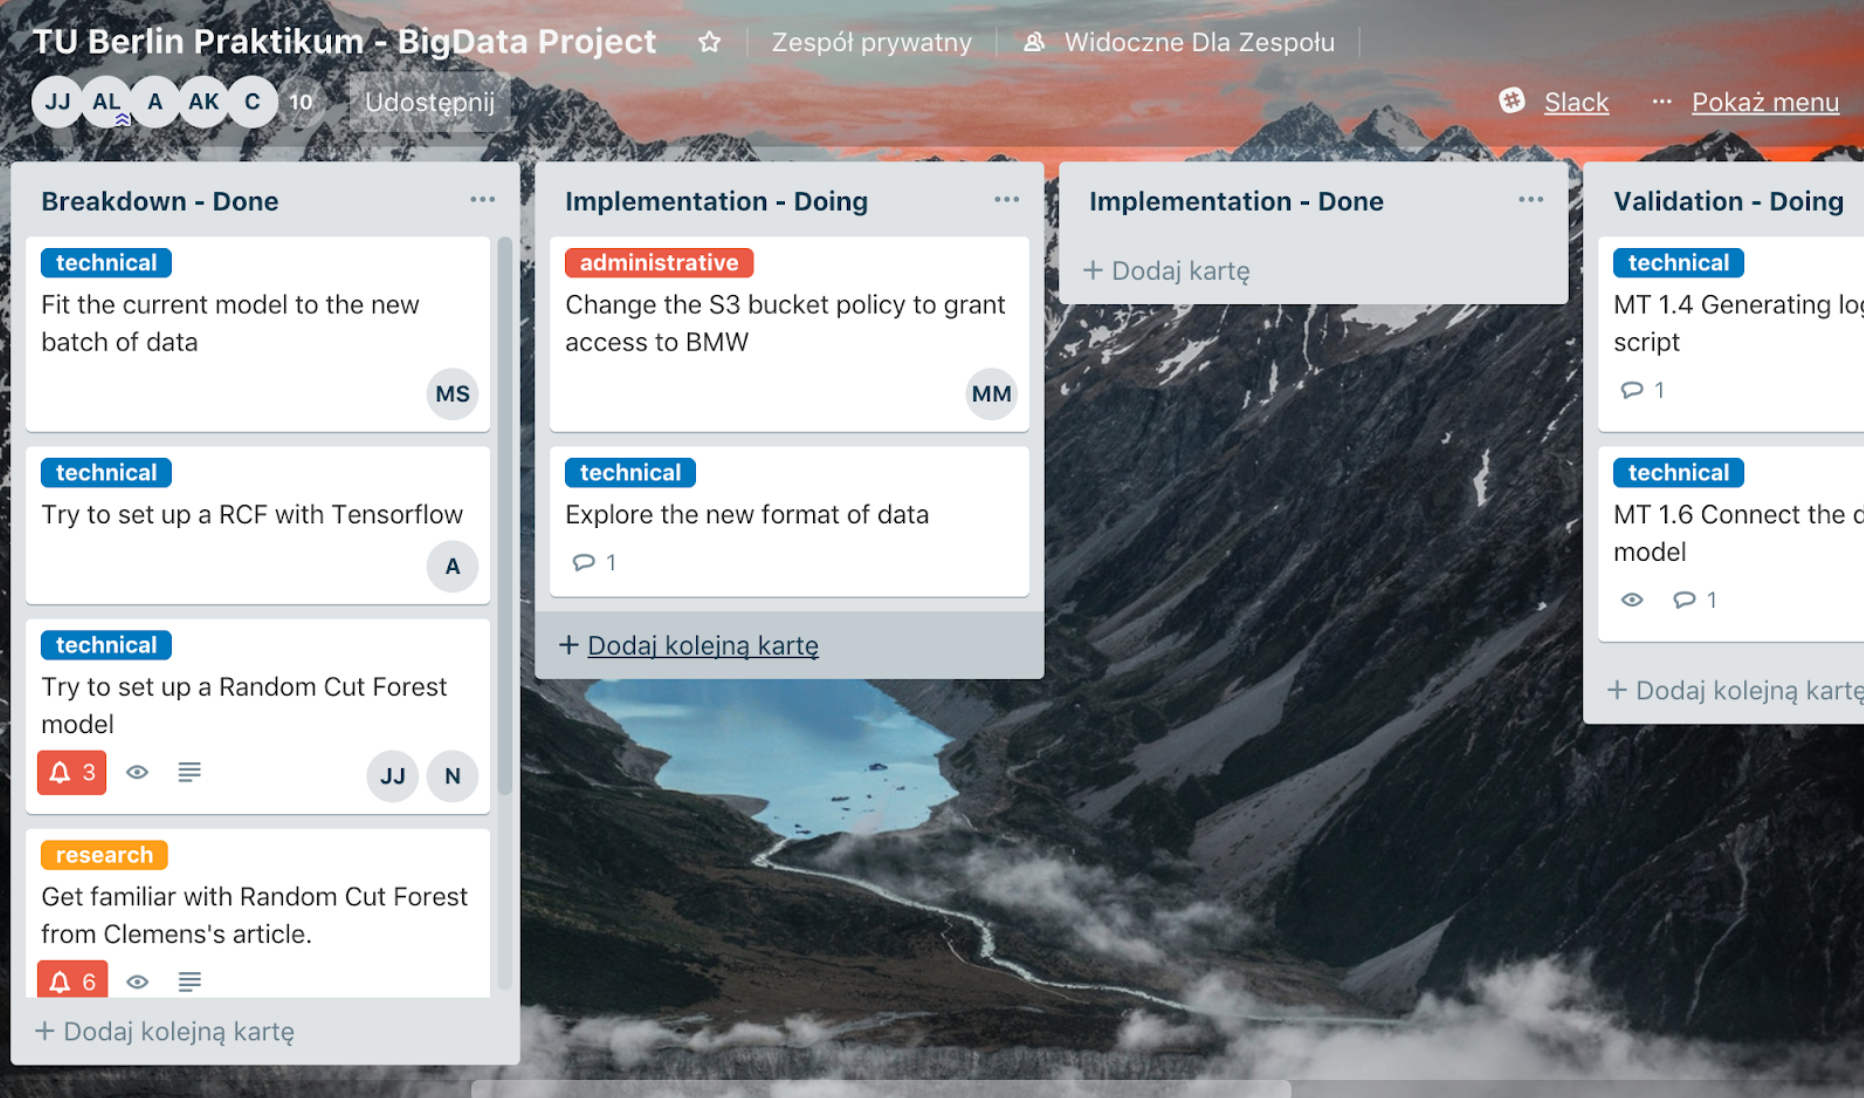
\includegraphics[width=1\textwidth]{images/trello.png}
        \caption{Big Data Analytics Trello board }
        \label{fig:trello_board_1}
    \end{figure}
    
After setting up the above mentioned columns, a user can start adding cards/user stories to the backlog. As seen in figure \ref{fig:trello_board_1}, Trello allows an user to add a title, a description (to detail the card), attachments, comments, due dates, responsible members and labels to a card.
It's worth noting, that for this project, the team used the board not just for programming related tasks. The Trello board was used for managing all project related assignments, for the purpose of registering each week's work.
\begin{figure}
    \centering
    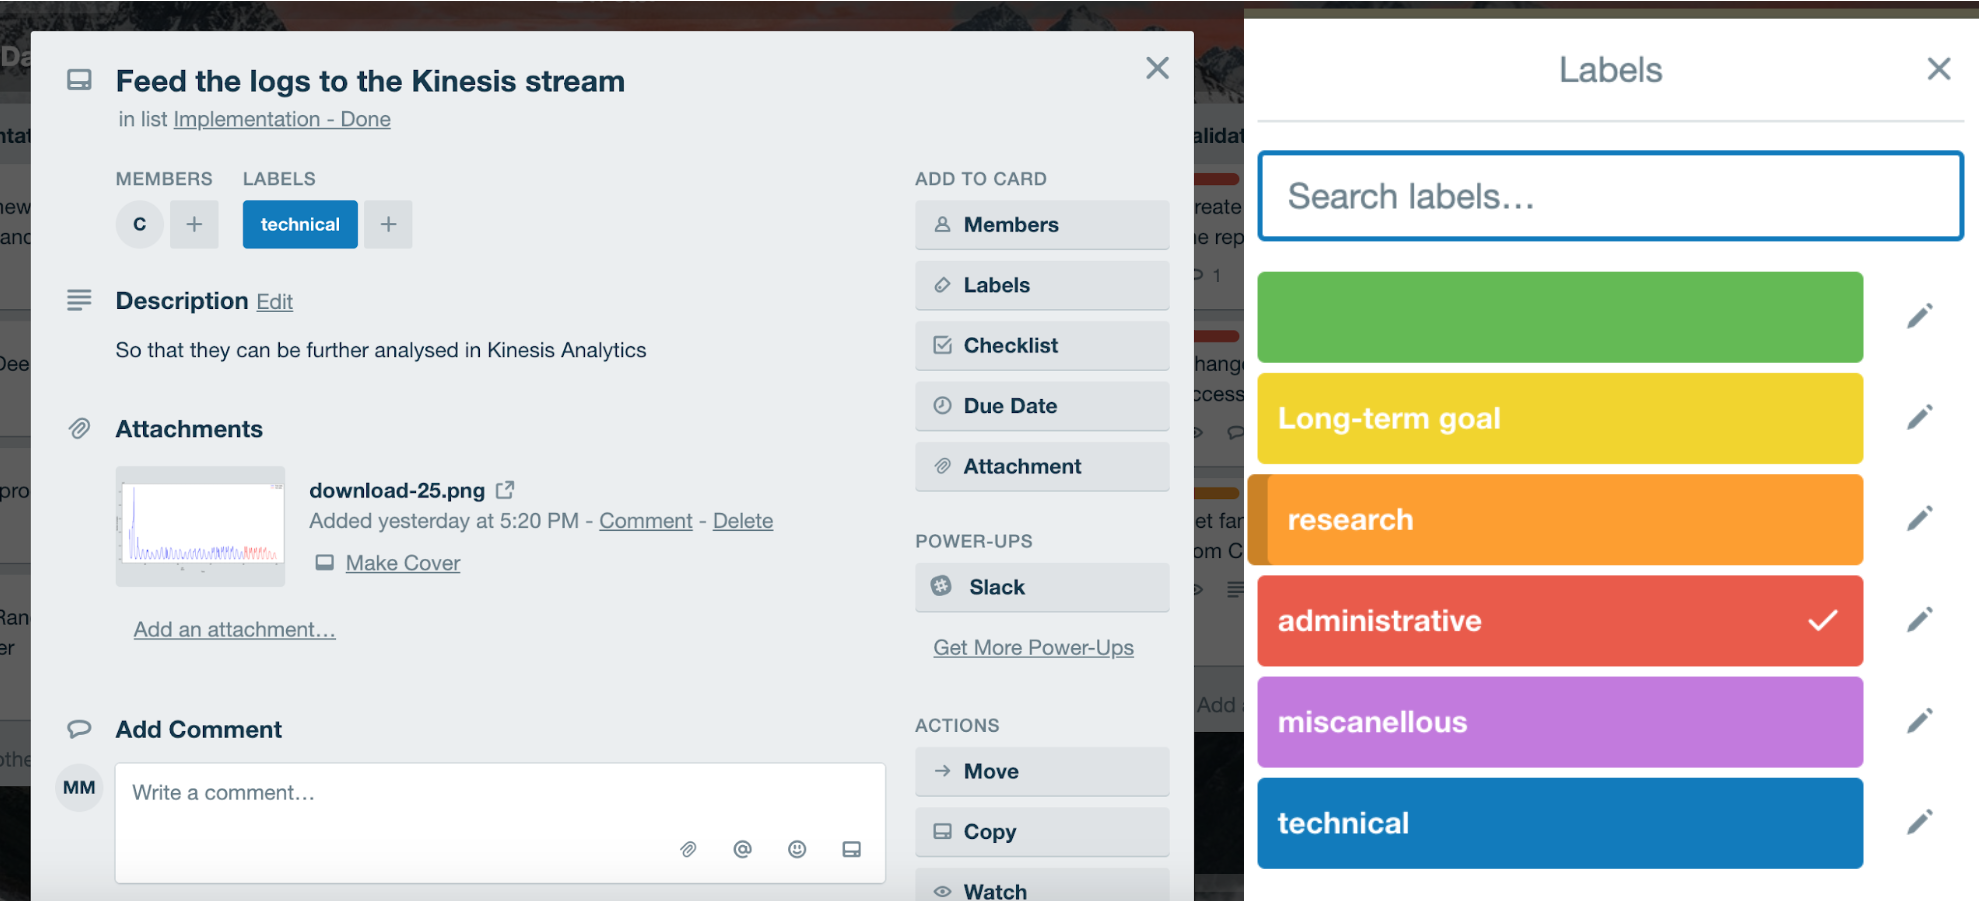
\includegraphics[width=1\textwidth]{images/card-view.png}
    \caption{Trello board card view with labeling details }
    \label{fig:fig:trello_board_2}
\end{figure}
In this project, the team used the following series of labels to mark the purposes of the user-story (see \ref{fig:trello_board_2}):
    \begin{itemize}
    \item \textbf{Long-term goal}: indicates that the card is most likely a use case in the project, which should be broken down further into smaller tasks
    \item \textbf{Research}: marks tasks that require the team to look for papers, documentation, solutions to solve certain impediments
    \item \textbf{Administrative}: highlights that a task has a managerial character
    \item \textbf{Technical}: indicates a developer task;
    \item \textbf{Miscellaneous}: used for any other subjects that a task can have, except the ones mentioned above (e.g. creating the presentation or documentation paper)
\end{itemize}
    
    \section{Real time anomaly detection with Kinesis - Clemens}
\label{sec:real_time_anomaly_detection}
    \subsection{Motivation}
    This approach is inspired by a Medium blog post\cite{MEDIUM}. 
    \footnote{\scriptsize{\url{https://medium.com/@devfire/real-time-anomaly-detection-in-vpc-flow-logs-part-1-introduction-55ed000e039b}}}
    The goal of the approach is to move the anomaly detection closer to a real-time setup. This means to continuously process the most recent data instead of analyzing data from the previous month or year to find anomalies. To give some more motivation about why this is actually an important issue, here is a quote from a job description from Netflix\cite{NETFLIX}:
    \begin{displayquote}
        "Netflix Operational Insight Team is the team responsible for building common infrastructure to collect, transport, aggregate, process and visualize operational metrics. We build powerful systems to allow everyone at Netflix visibility into the state of our environment at both a macro and micro level."
    \end{displayquote}
    The fact that a leading and modern company like Netflix builds a whole team just dedicated to checking and visualizing the current system state in real time, underlines how important it is to know at every moment how your environment performs.\\
    AWS Kinesis is a very suitable tool for this problem for multiple reasons. First of all, Kinesis is designed to process streaming data. This means we can ingest real-time data which is a perfect fit for our given VPC flowlog data. Second Kinesis comes with Kinesis Data Analytics already built in. Amazon Kinesis Data Analytics offers easy ways to analyze streaming data, gain actionable insights, and respond to business needs in real time. In addition to that there is a SQL function called “Random cut forest with explanation” which is described by AWS as follows:
    \begin{displayquote}
        Computes an anomaly score and explains it for each record in your data stream. The anomaly score for a record indicates how different it is from the trends that have recently been observed for your stream. The function also returns an attribution score for each column in a record, based on how anomalous the data in that column is. For each record, the sum of the attribution scores of all columns is equal to the anomaly score. \cite{awsRcf}
    \end{displayquote}

    \subsection{Architecture}
    So with this prior knowledge let’s jump right into the system setup.
    First let’s get an overview of the system as it was implemented during the project phase:
    \begin{figure}
        \centering
        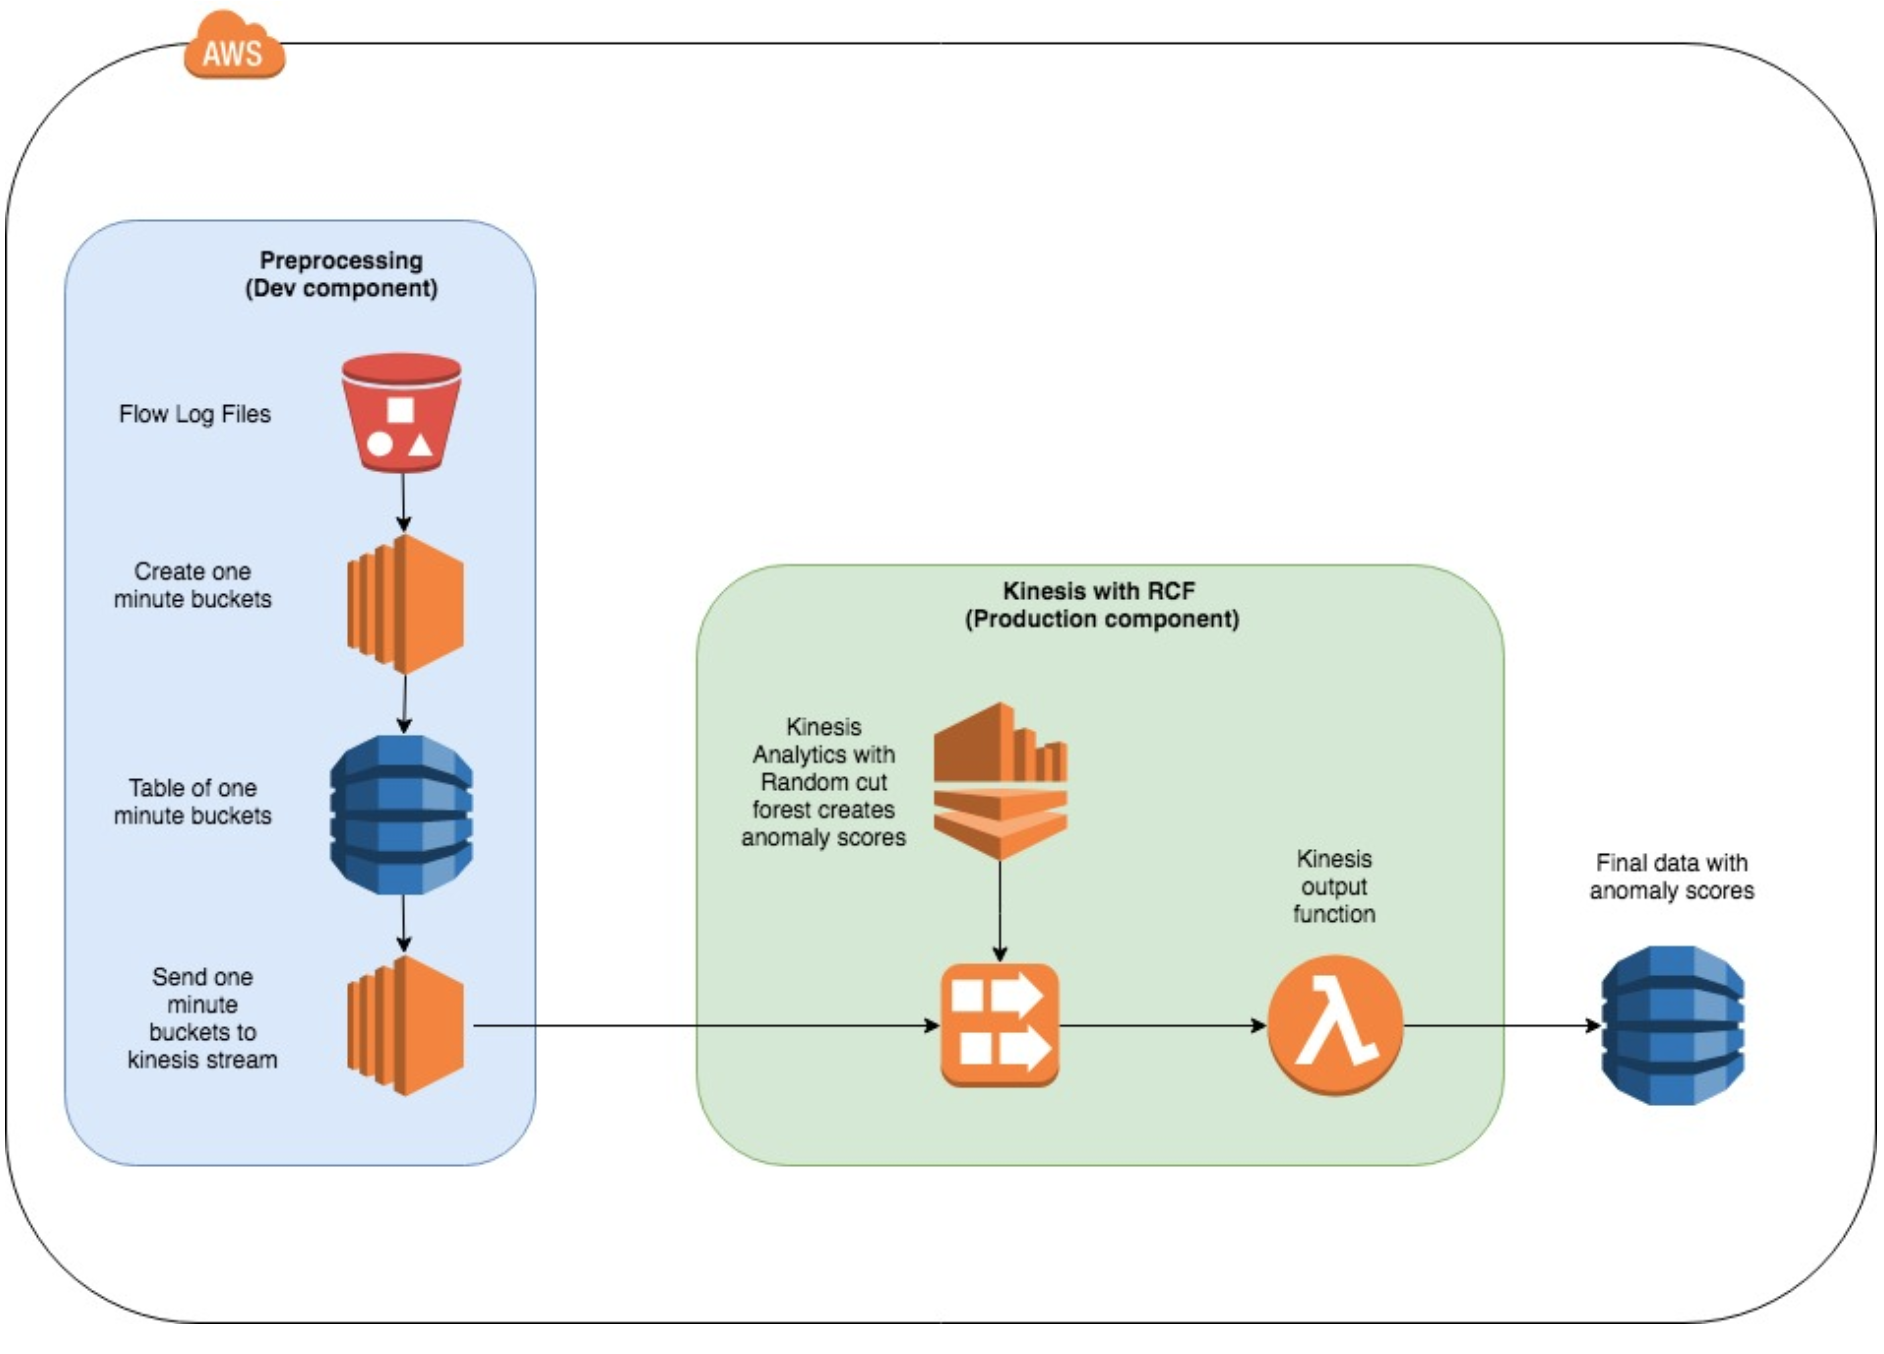
\includegraphics[width=1\textwidth]{images/medium-kinesis-setup.png}
        \caption{Medium Kinesis Random Cut Forest Setup}
        \label{fig:medium_kinesis_setup}
    \end{figure}
    \FloatBarrier
    First of all it should be noted that all the preprocessing components on the left (blue area in figure \ref{fig:medium_kinesis_setup}) would not be part of a production system. In a production system we would have a continuous stream of VPC flow logs which needs to be handled and preprocessed, whereas in the project setup we had all the flow logs data from the past in a S3 bucket. 
    
    \subsection{Preprocessing components (blue area in figure \ref{fig:medium_kinesis_setup})}
    In the following section we will look at the preprocessing setup in detail, keeping in mind that this is not created to run in production.
    
    \paragraph{S3: Flow Log Files}
    All the flow logs data provided by BMW lies in an S3 bucket called \textit{fog-bigdata-bmw-data}. As mentioned in \pageref{sec:fixed_data}, there are two types of data: first the metrics, which already contain summaries about how many requests were made to the system during a certain time interval. Another issue here was, that the time intervals are of different size (sometimes five minutes, sometimes four or six or something similar). Of course this is not a good basis to run our anomaly detection, because we cannot know what value we expect (since the size of the intervals are different). Therefore the second type of data is more suitable, namely the raw VPC Flowlogs. However, we want to look at how many requests are made to our system per minute and therefore we need to do some preprocessing.
    
    \paragraph{EC2: create one minute buckets}
    This is where the first script with the name \textit{createOneMinuteBuckets.py} comes in. This script is executed on an EC2 instance and reads all the flow log records from the S3 bucket. It creates one-minute buckets from the Flowlogs, so that we know for every one minute time interval how many requests were made to the system. 
    
    \paragraph{DynamoDB: table of one minute buckets}
    The information about these one minute buckets is then written into a DynamoDB table (called \verb|medium_bmw_data_to_kinesis|). For the sake of this project the data from the Kinesis table was then exported to a CSV file and the information about the weekdays was added (currently done in Excel). This means that for every one minute bucket we know the hour and the minute and also on which weekday it was recorded. This might be relevant because the expected number of request at 8am on a Sunday can be very different than 8am on a Monday, especially because the requests come from driving cars.  Of course this step will not be part of a production system (as mentioned before).
    
    \paragraph{EC2: send one minute buckets to Kinesis stream}
    The next script is called \textit{generateAnomalyScores.py}. The script and the final CSV file is uploaded to EC2 again. The script takes the data from this CSV file and sends it to the kinesis Stream called medium\textunderscore VPCFlowLogs. An alternative setup could be to read the data directly from DynamoDB and add the information about the weekday in the python script (instead of using CSV and Excel).\\
    This is where the preprocessing part (which would look different in a production system) ends and where the production component (green area in figure \ref{fig:medium_kinesis_setup}) comes into play.\\
    
    \subsection{Production component (green area in figure \ref{fig:medium_kinesis_setup})}
    In this section we assume that we already have all the data we need in the right format. This is the part of the system where the actual anomaly detection happens. This part of the the setup can be used in a production environment in the same or in a similar way. All the preprocessing is done and the data is already fed into the our Kinesis stream.
    \begin{figure}
        \centering
        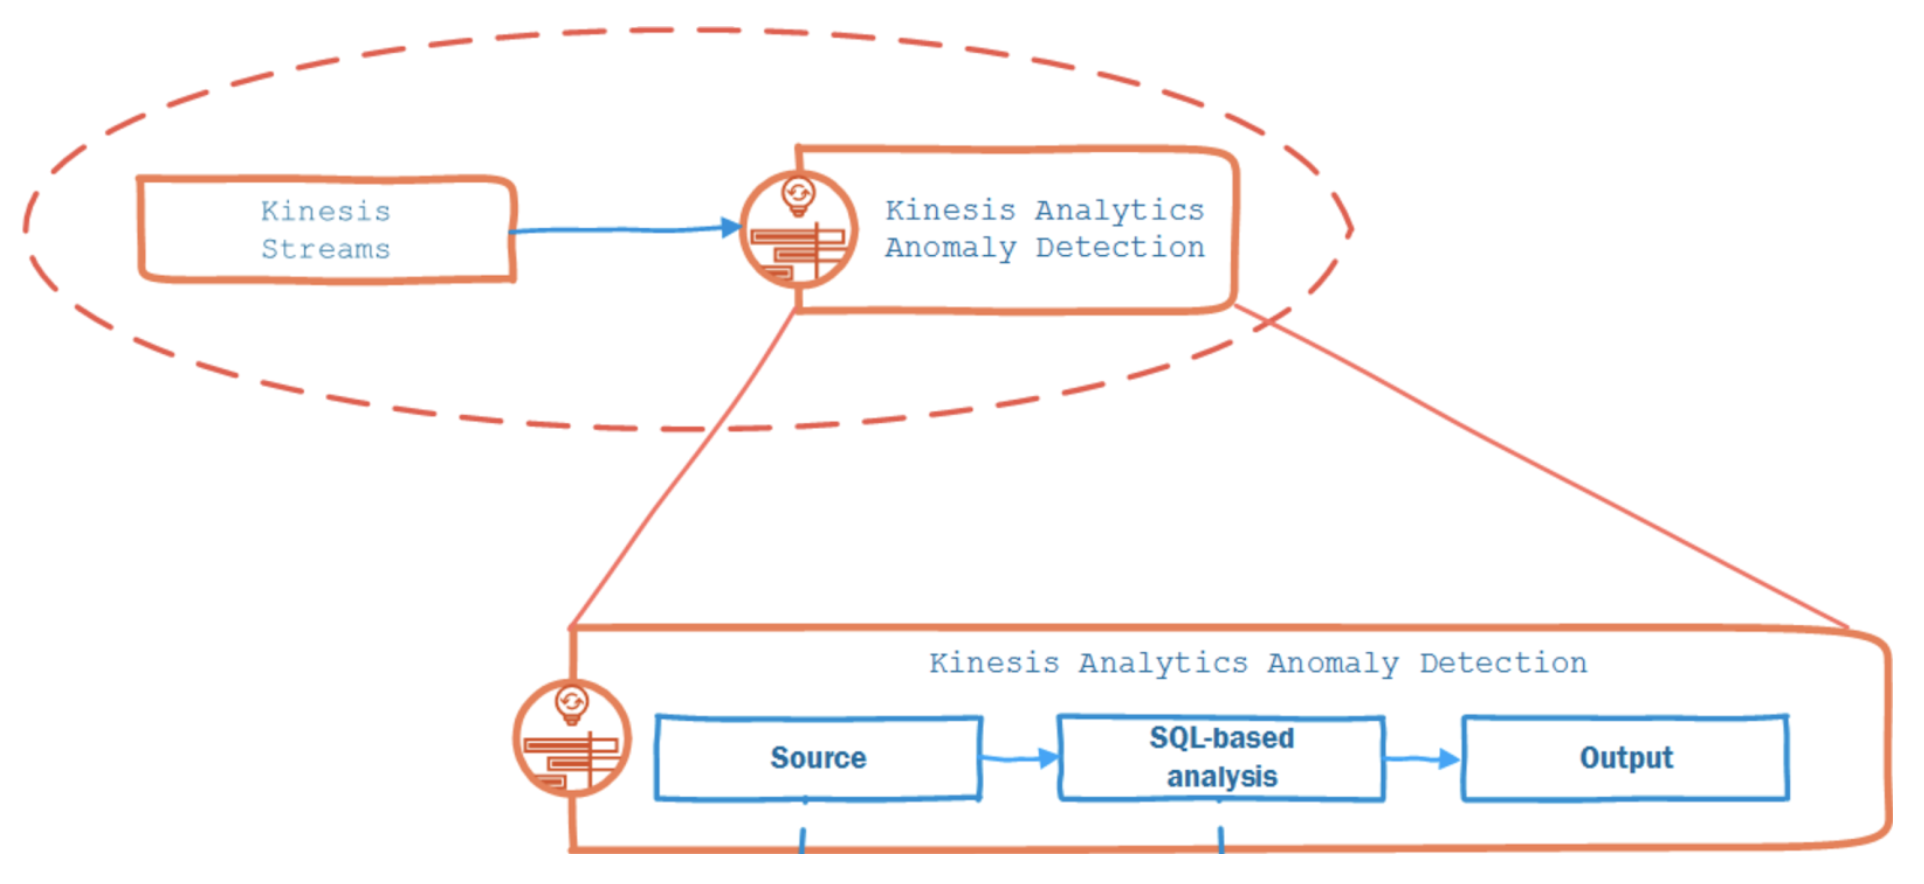
\includegraphics[width=1\textwidth]{images/kinesis-rcf.png}
        \captionsource{Kinesis Data Analytics with RCF}{\scriptsize{Source: https://medium.com/@devfire/real-time-anomaly-detection-in-vpc-flow-logs-part-5-anomaly-detection-d1fc9b61baf8}}
        \label{fig:medium_kinesis_data_analytics_rcf}
    \end{figure}
    \FloatBarrier
    The Kinesis stream has a Kinesis Data Analytics application which sends the data to random cut forest where the anomaly scores are created. This is the SQL code for the real time analytics:
    \begin{figure}
        \centering
        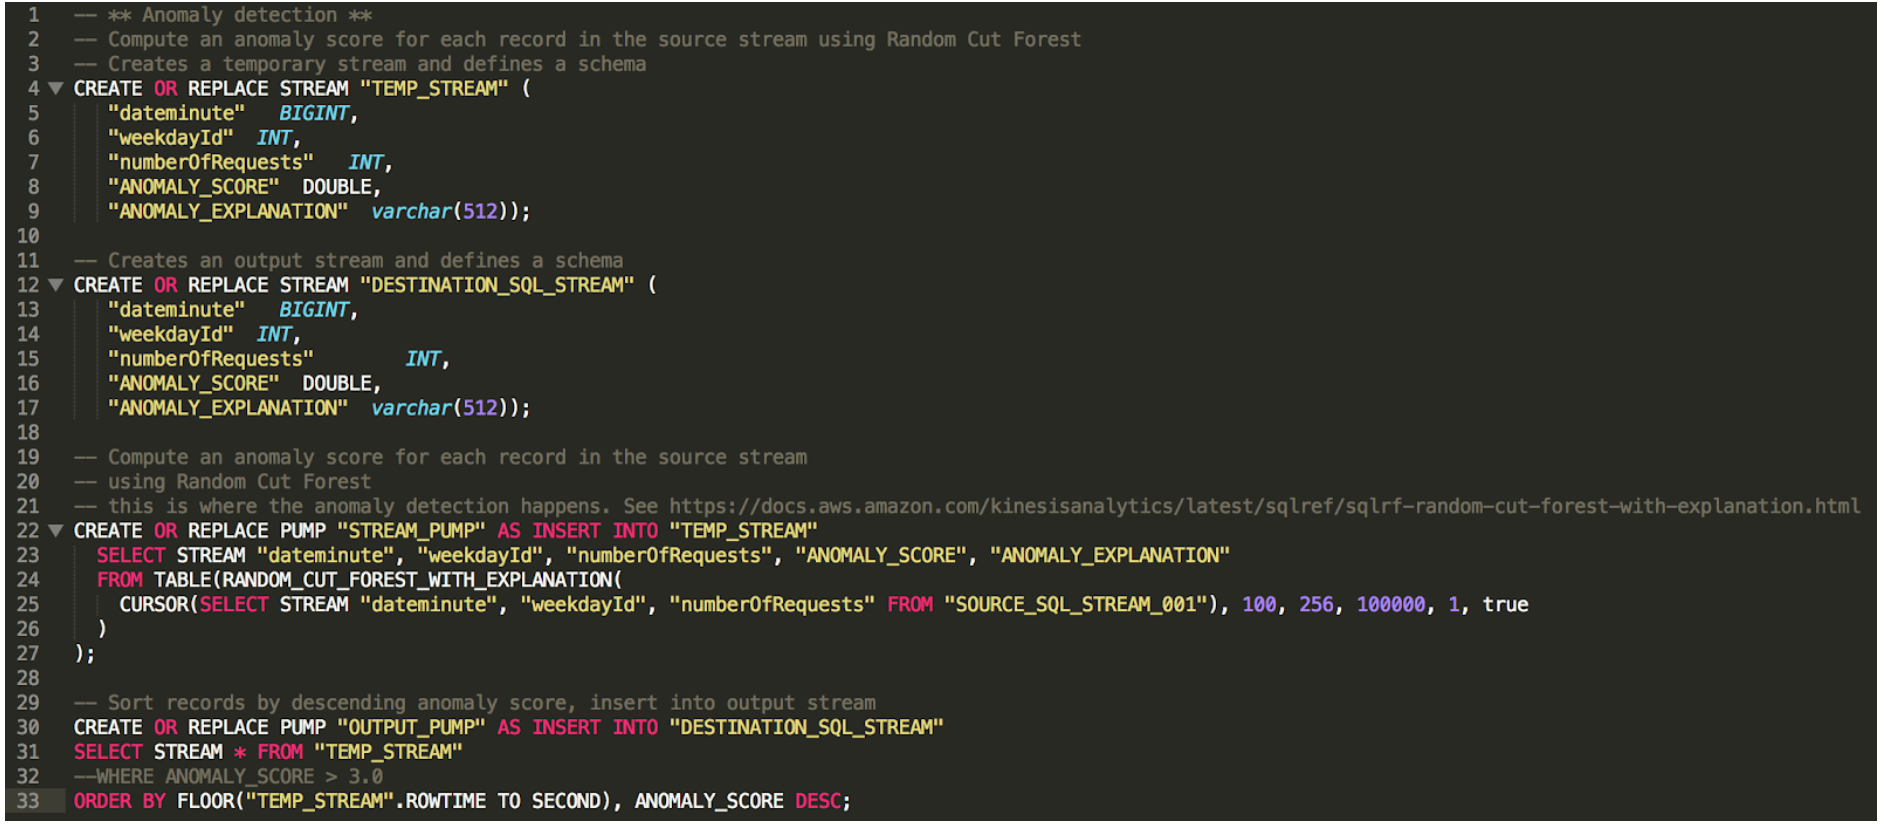
\includegraphics[width=1\textwidth]{images/sql-analytics.png}
        \captionsource{SQL code for real time analytics}{\\\scriptsize{Source: https://medium.com/@devfire/real-time-anomaly-detection-in-vpc-flow-logs-part-5-anomaly-detection-d1fc9b61baf8}}
        \label{fig:medium_sql_analytics}
    \end{figure}
    \FloatBarrier
    As we can see from the comment in line 32 it would be possible to already define a threshold here. This would then mean, that only anomaly scores which are higher than that specified threshold are sent to the output stream. However it is recommended to do implement this threshold in the output lambda function, to keep the threshold logic separate from the creation of the anomaly scores. Furthermore it is a lot easier to version and backup the lambda function in case the threshold is changed over time than to maintain different versions of the SQL code in the Kinesis Data Analytics part.
    \paragraph{Lambda: Kinesis output function}
    The output of the kinesis stream is sent to the Lambda function \verb|medium_bmw_kinesis_to_dynamodb_2|. \\
    This Lambda function just stores the results to another DynamoDB called \verb|kinesis_bmw_anomaly_scores|. Obviously this last database table was just for the purpose of the project phase to collect all the anomaly scores and visualize them in a graph but it is not needed in a production setup (as indicated in the system architecture). Instead in a production system this output function should contain the threshold for the anomaly score and then send a message or trigger a phone call if the threshold is exceeded.
    
    \subsection{Results}
    \begin{figure}[h]
        \centering
        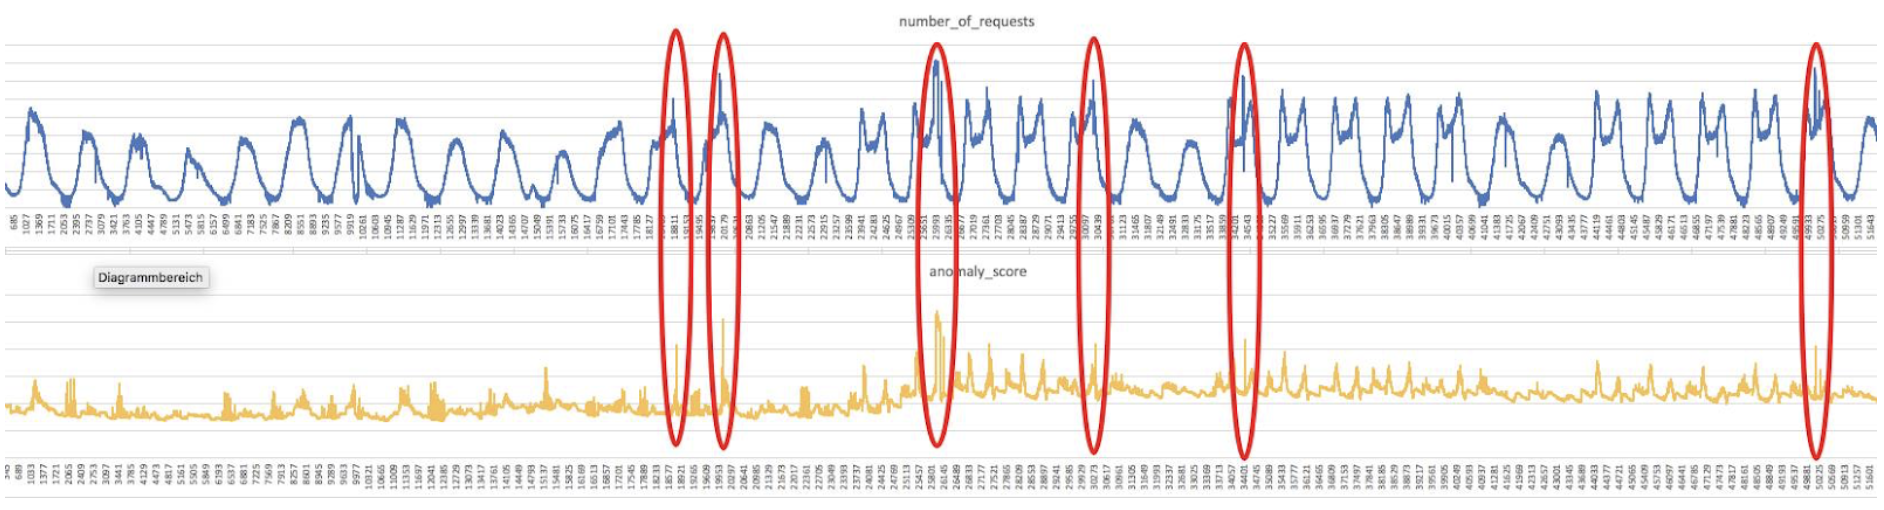
\includegraphics[width=1\textwidth]{images/kinesis-results.png}
        \caption{Visualisation of Kinesis Analytics Results}
        \label{fig:medium_kinesis_results}
    \end{figure}
    \FloatBarrier
    The blue graph at the top of figure \ref{fig:medium_kinesis_results} shows the requests to the the system per minute (from the one minute buckets). The orange graph at the bottom of figure \ref{fig:medium_kinesis_results} visualizes the anomaly score at that time. This means if we see an unexpected high peak or unexpected low drop in the first graph (number of requests per minute), in both cases we would expect a peak in the second graph (the anomaly scores). All in all this example does not show a perfect result (since we would expect our anomaly scores to be consistently low when there is no anomaly), however we have to take into account that this particular data set show the requests from December 21, 2018 until January 28, 2019 which means that it starts with the Christmas holidays which does not show the normal pattern of five weekdays followed by two weekends which we see towards the end.\\ Furthermore this is a series of 54,689 one minute buckets which is not a very long series to train on. Despite these factors of having limited and atypical data the high spikes in the anomaly scores (highlighted by the red ellipses) indicate that the approach in general is quite promising and that it can already detect anomalies.
    
    \subsection{Future work}
    The presented results are retrieved from feeding the data into the random cut forest in the following format: date-minute data, the weekday ID (as an integer) and number of requests.
    To refine the system further it might be interesting to try different combinations of these three input variables to see which combination gives the best results. This way it could be determined if it decreases the performance if we leave out the information about the weekday completely for example.
    
    \subsection{Implementation guide (Kinesis Random Cut Forest)} 
    This can be found in the appendix of this report (Appendix \ref{appendix-medium}) or online at \url{https://gist.github.com/clemenspeters/8e9025e3bd71e9087df154fb06f96328}
    \section{Anomalies detection algorithms}
        \subsection{Amazon SageMaker Random Cut Forest - Nursultan}
            The code for the instructions below is in GitHub repository:
\begin{itemize}
    \item \textit{models$\setminus$random\textunderscore cut\textunderscore forest$\setminus$rcf\textunderscore bmw\textunderscore train\textunderscore deploy.ipynb} - the notebook contains a set of scripts to train and deploy the RCF model
    \item \textit{models$\setminus$random\textunderscore cut\textunderscore forest$\setminus$rcf \textunderscore test\textunderscore endpoint\textunderscore model.ipynb} - the notebook contains a set of scripts to test the deployed model
\end{itemize}
Amazon Sagemaker RCF is an algorithm designed to detect anomalous data points within a dataset. 
This section describes a creation and a deployment of a SageMaker RCF model. 
The data consists of a number of requests (VPC Flowlogs from BMW) aggregated into one minute buckets. To train the model, we used the data over the course of one week that represents a normal pattern. Then, we fed the whole data into the trained model for testing.\\To start with, it is necessary to specify the locations where we will store our training data and trained model artifacts. In particular, we need the following data:
\begin{itemize}
    \item bucket - An S3 bucket accessible by an account.
    \item prefix - The location in the bucket where a notebook's input and output data will be stored. (The default value is sufficient.)
\end{itemize}
\begin{figure}[h]
    \centering
    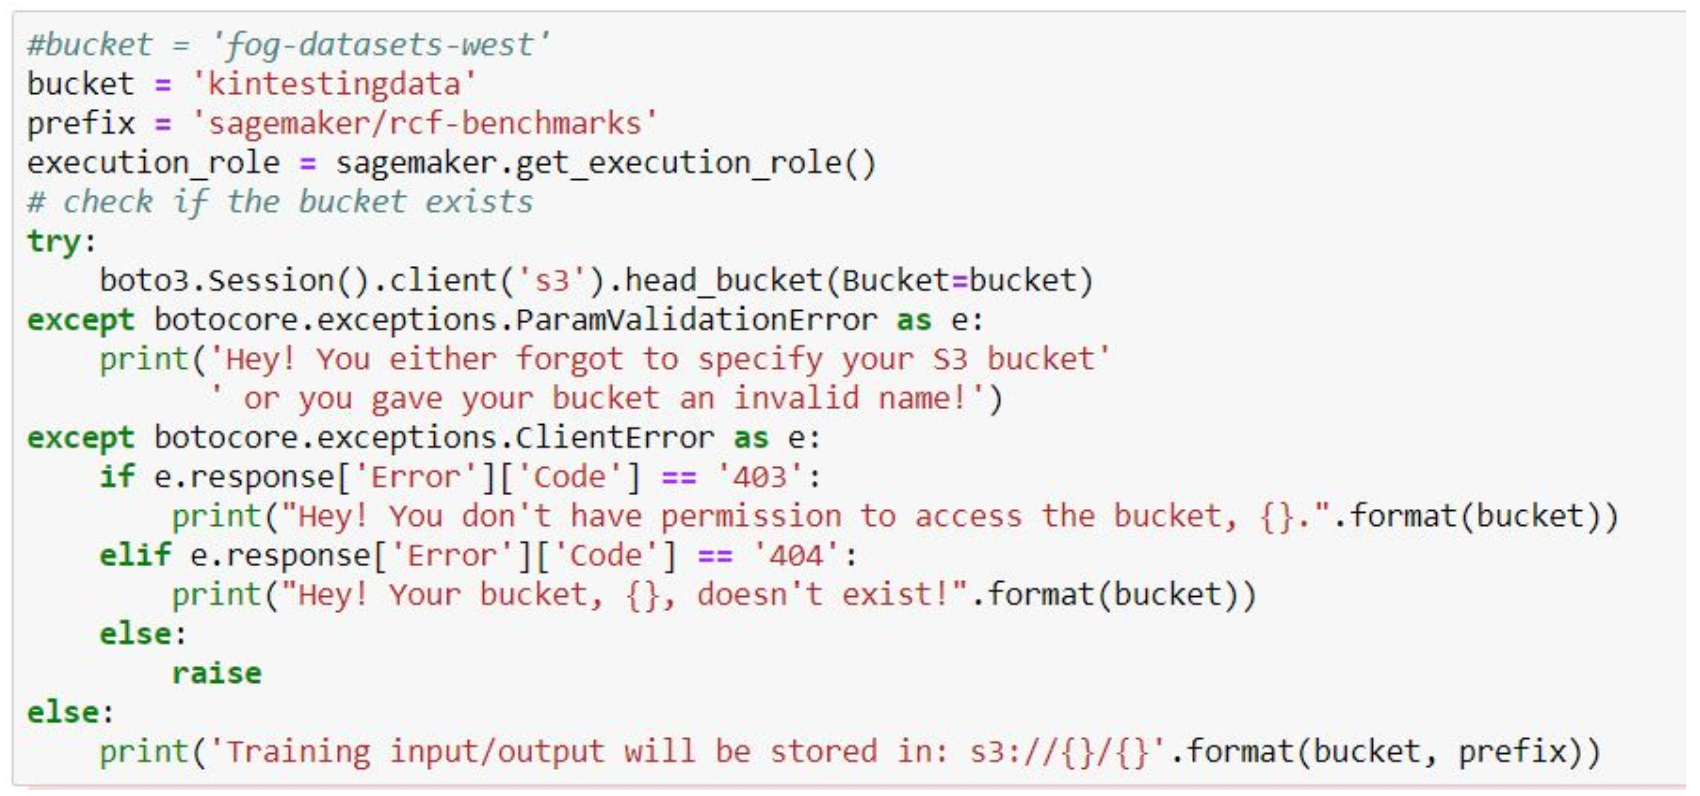
\includegraphics[width=1\textwidth]{images/rcf-data-location.png}
    \caption{Specifications for data location}
    \label{fig:rcf_data_location}
\end{figure}
Next, we configure a SageMaker training job to train the Random Cut Forest (RCF) algorithm on one minute data.

\textbf{Hyperparameters}\\
Particular to a SageMaker RCF training job are the following hyperparameters:
\begin{itemize}
    \item \textit{num\textunderscore samples\textunderscore per\textunderscore tree} - the number of randomly sampled data points sent to each tree. As a general rule, 1/\textit{num\textunderscore samples\textunderscore per\textunderscore tree} should approximate the estimated ratio of anomalies to normal points in the dataset.
    \item \textit{num\textunderscore trees} - the number of trees to create in the forest. Each tree learns a separate model from different samples of data. The full forest model uses the mean predicted anomaly score from each constituent tree.
    \item \textit{feature\textunderscore dim} - the dimension of each data point.
\end{itemize}
Along with these RCF model hyperparameters, we provide additional parameters defining things like the EC2 instance type on which training will run, the S3 bucket containing the data, and the AWS access role. Note that,
\begin{itemize}
    \item Recommended instance type: ml.m4, ml.c4, or ml.c5
    \item Current limitation: The RCF algorithm does not take advantage of GPU hardware.\footnote{ https://docs.aws.amazon.com/sagemaker/latest/dg/randomcutforest.html}\\
\end{itemize}
\begin{figure}[h]
    \centering
    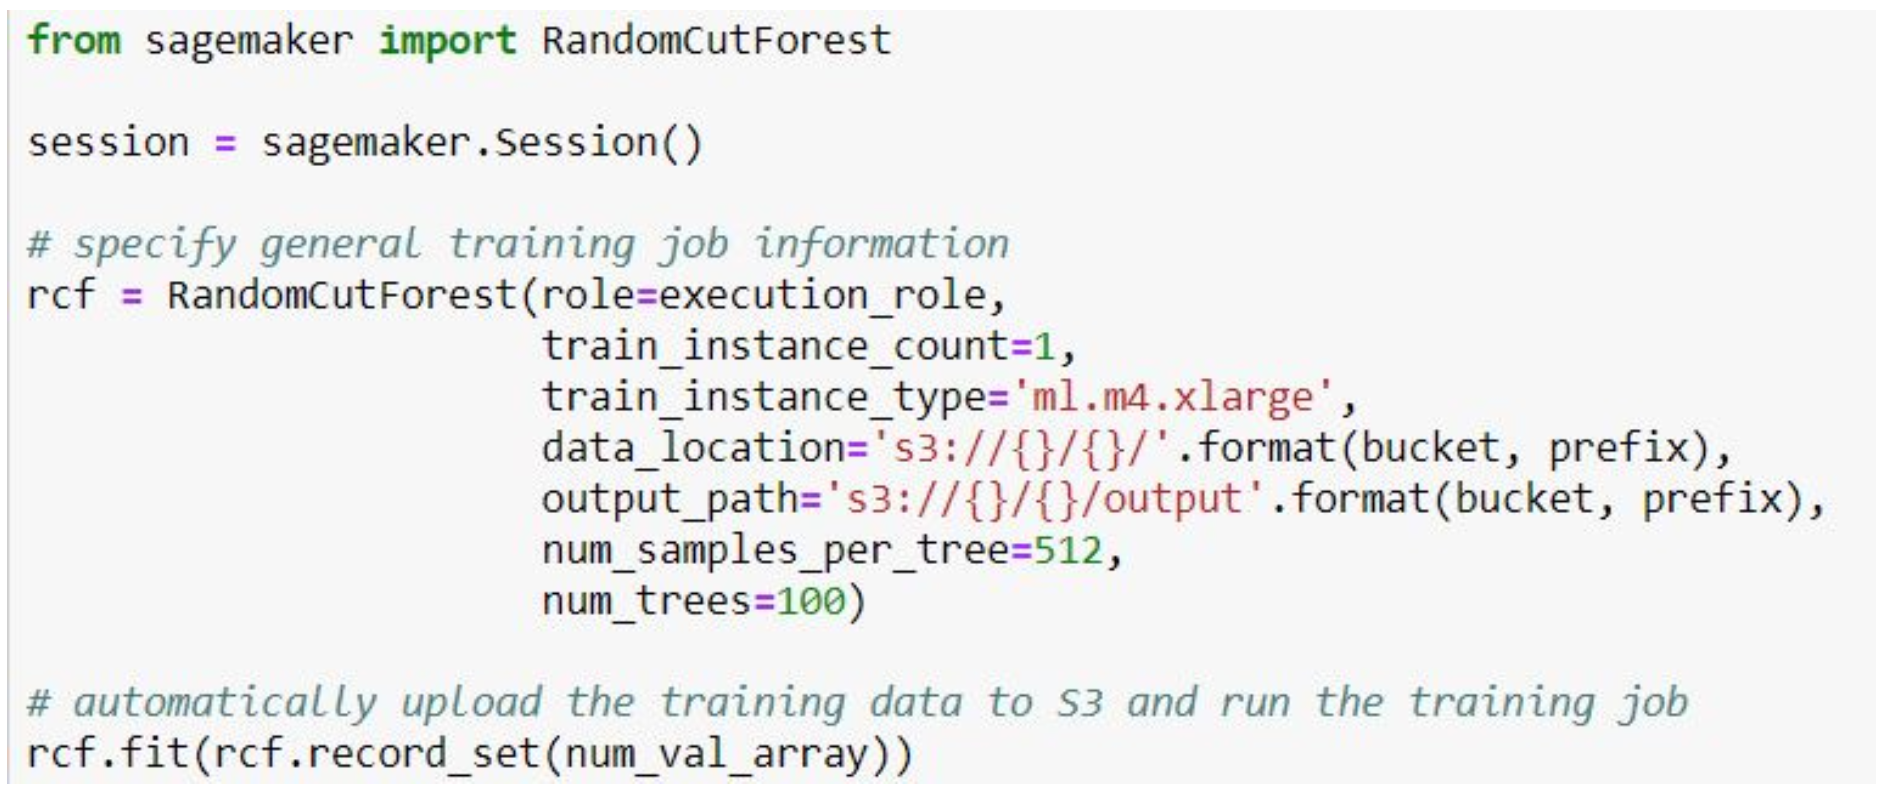
\includegraphics[width=1\textwidth]{images/rcf-model-training.png}
    \caption{RCF Model training}
    \label{fig:rcf_model_training}
\end{figure}
We used SageMaker Python SDK deploy() function from the job to create an inference endpoint. The function has two input parameters:  the instance type and an initial number of instances. 

There are two ways to invoke the trained model:
\begin{itemize}
    \item Right after training in the same notebook, calling a job’s \textit{predict(Test\textunderscore data)} function
    \item From elsewhere(e.g., inside a lambda function), using a function \textit{runtime.invoke\textunderscore endpoint\\(EndpointName, ContentType, Body)}
\end{itemize}
The model outputs an anomaly score for each input data point. It is suggested in a RCF documentation, to compute a value of the anomaly threshold as 3 standard deviations from the mean score. Any value that is beyond the threshold is considered as an anomaly. 
The way to compute the threshold value is subject to change. Depending on business requirements, one can calculate it either once for the whole period of data, or for shorter periods of time, e.g., recompute threshold every day.\\We decided to experiment and calculate the threshold per each day and these results are available below.
The first following plot represents the data, the second one demonstrates testing results. The red plot depicts threshold values that we compute for each day. As we can see, not only high local peaks are detected as anomalies, but also local downfalls and congestions on bottoms are anomaly candidates. 
\begin{figure}[h]
    \centering
    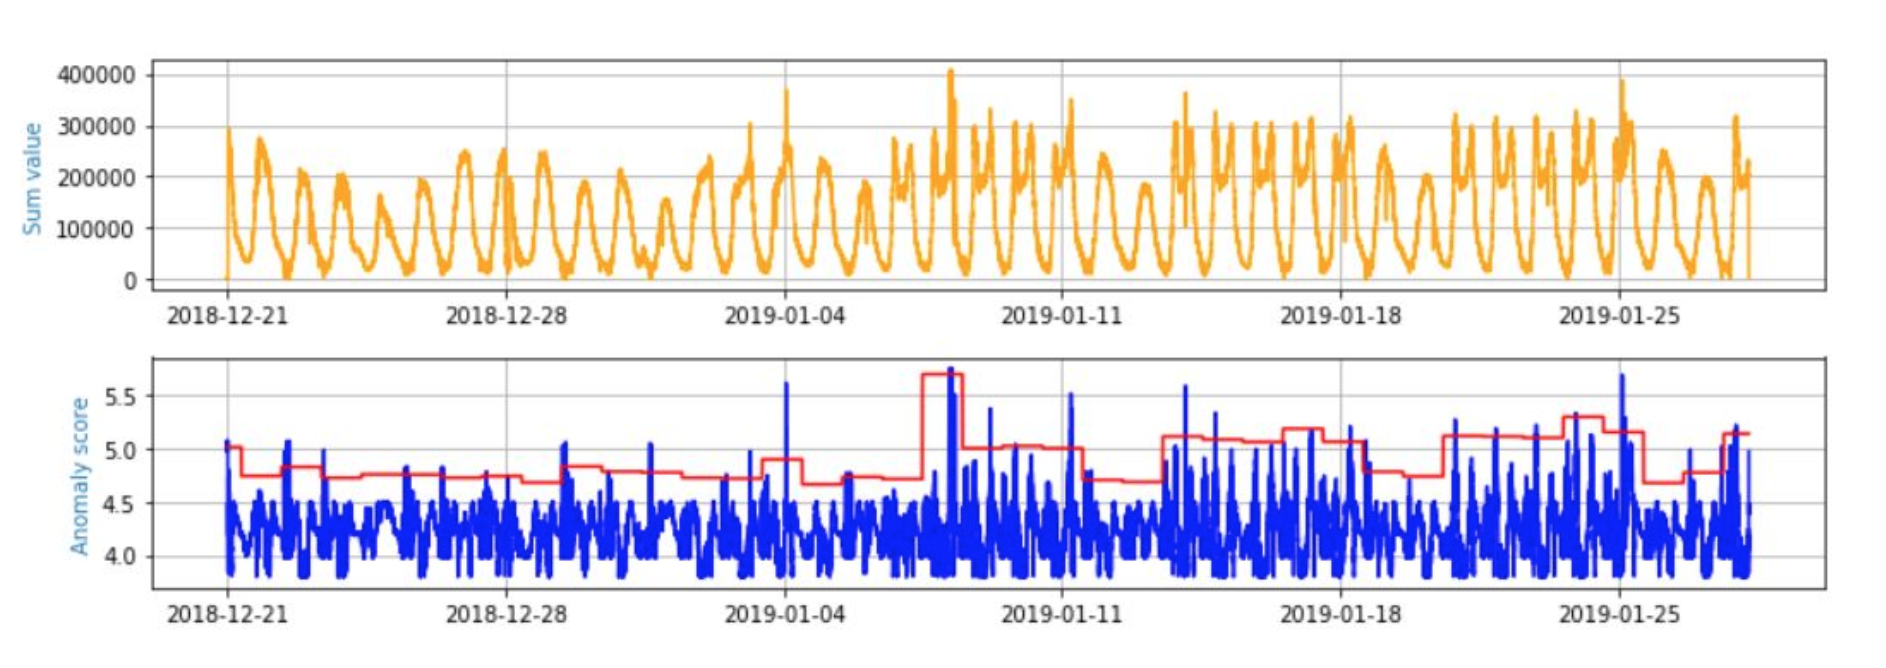
\includegraphics[width=1\textwidth]{images/rcf-results.png}
    \caption{Plotted data, anomaly scores, and anomaly threshold values}
    \label{fig:rcf_results}
\end{figure}
\FloatBarrier



            \FloatBarrier
            
        \subsection{Mean Predictor Algorithm - Marius}
            %Author: Marius
\textit{Author: Marius Schidlack} \\
\label{mean-predictor}
\paragraph{Motivation}
While sophisticated algorithms like the random cut forest seem to be promising for fitting large amounts of data with complex patterns, they did appear overly complicated for the amount and nature of the data at hand. The data shows a clear weekly periodicity, where the data from one week can hardly be distinguished from another. The only exception is the one week of holidays. In fact, the weeks are so similar, that we can predict the same pattern every week with high confidence. This was the motivation for us to implement a very simple, yet effective machine learning model called the Mean Predictor.

\paragraph{Idea}
The main idea is already contained in the name Mean Predictor. The objective of the Mean Predictor is to calculate the expected week and standard deviation for each point in a week. Accordingly, we can identify outliers by simply checking if the data point lies within the allowed deviation of the expected value. 

Unfortunately, AWS Sagemaker does not offer a Mean Predictor as an Out-Of-The-Box algorithm like the Random Cut Forest. Thus, we implemented it ourselves.

\paragraph{Implementation}

\begin{figure}
    \centering
    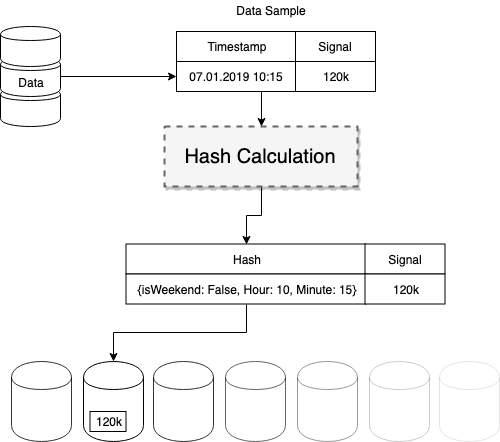
\includegraphics[width=0.6\textwidth]{images/mean_predictor_hashing.png}
    \caption{Hashing process of Mean Predictor Model}
    \label{fig:mean_predictor_hashing}
\end{figure}

For calculating the expected week, we sorted every data point into a bucket that is determined by its \textit{Timestamp}. Each bucket has a hash or index associated with them. After distributing all the data into buckets, we calculate the mean of all the values in one bucket, as well as a measure of standard deviation. This process is visualized in figure \ref{fig:mean_predictor_hashing}.

The hashing function is central to this approach, as we can arbitrarily craft the features that we want our mean predictor to represent. Apart from the weekly periodicity of the data, we also noticed a very predictable daily pattern throughout the working week. Hence we decided to put all working days into one set of buckets and all weekend days into a different set. We did this to ensure a reasonable amount of samples for each bucket. The hashing function currently employed in the mean predictor is shown in  code example \ref{lst:timestamp_hashing}. As more and more data comes in, the function can be adjusted if necessary.

% wrap in minipage so the code doesnt get split to multiple pages
\begin{minipage}{\linewidth}
\begin{lstlisting}[caption={Time stamp hashing function used for Mean Predictor},label={lst:timestamp_hashing}]
def __time_hash(self,t):
       return (t.weekday() < 5,t.hour,t.minute)

\end{lstlisting}
\end{minipage}

As mentioned before, we also require a measure of expectation deviation for determining outliers. The first thing that comes to mind is the standard deviation:

\begin{equation}
\begin{aligned}
\sigma_t = \sqrt{\frac{1}{n}\sum_{i=1}^N (s_t^{(i)} - \mu_t)^2}\\
\end{aligned}
\end{equation}

Where $\mu_t$ denotes the mean value of bucket $t$ and $s_t^{(i)}$ the $i$-th value in this bucket. However, since we square the distance from the mean, the standard deviation weighs outliers much heavier than conform data, which might not be the desired behaviour for the task at hand, because outliers are what we want to detect. Instead one might want to use the average euclidean distance from the mean:
\begin{equation}
\begin{aligned}
\sigma_t = \frac{1}{n}\sum_{i=1}^N \sqrt{(s_t^{(i)} - \mu_t)^2}\
\end{aligned}
\end{equation}
In our case, the choice of deviation measure had little influence on the final results, nevertheless if future training data is noisy and contains a lot of outliers, this might be an option to consider. 

\paragraph{Training and Prediction}
\begin{figure}[h]
    \centering
    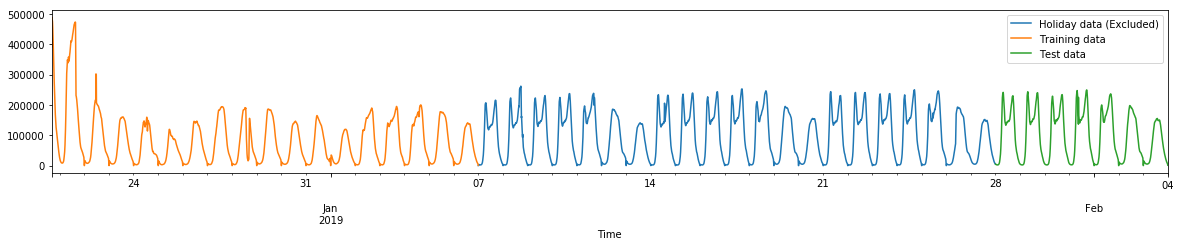
\includegraphics[width=1\textwidth]{images/mean_pred_training_data.png}
    \caption{Train-Test split of data used for the mean predictor}
    \label{fig:mean_predictor_training_data}
\end{figure}
Due to the fact that the Christmas holidays are included in the data, a lot of the provided training data is anomalous and therefore not useful for training a model that is supposed to detect anomalies. Accordingly, we excluded this data from training, leaving us with only three weeks of training data. Alternatively one could also alter the hashing function to give holidays a separate set of buckets. Our train-test split is shown in figure \ref{fig:mean_predictor_training_data}.

\begin{figure}
    \centering
    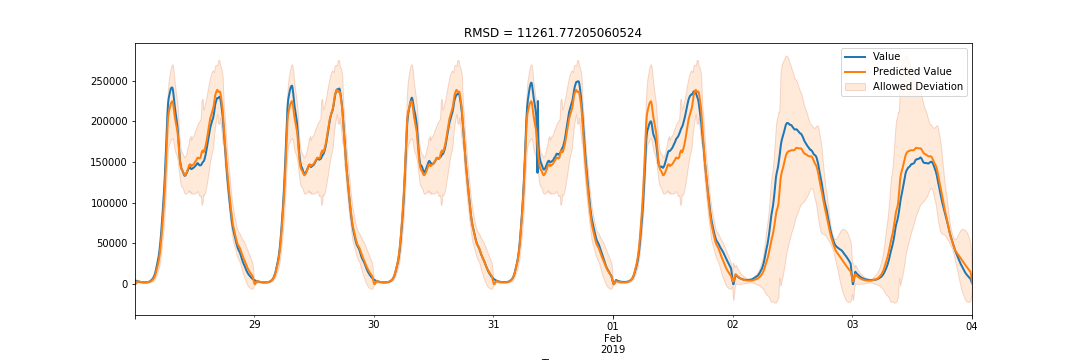
\includegraphics[width=1\textwidth]{images/mean_pred_test.png}
    \caption{One week prediction of Mean Predictor model}
    \label{fig:mean_predictor_prediction}
\end{figure}

Once we have expected value and deviation for each bucket, making predictions is trivial. The model simply takes a time interval and calculates the hash for each timestamp within that interval. We obtain the prediction by simply looking up the expected value and deviation in our table. Figure \ref{fig:mean_predictor_prediction} depicts a prediction for the week starting at the 28th of January 2019 (test set) and compares it to the ground truth. For this test data, the prediction is highly accurate and the true values never leave the confidence interval. The RMSE \textit{(Root Mean Squared Error)} of the prediction lies around 11,261. Further investigation is needed to accurately assess the outlier detection performance, since we were lacking test data that contains real outliers. For the time being, by looking at the confidence interval, we can see that sudden spikes or lows in the timeseries could easily be identified as anomalies.
\pagebreak

\paragraph{Deployment as Sagemaker Endpoint}
In order to use our model in the Cloud, we deployed it as an AWS Sagemaker Endpoint. In the following we describe the technical details related to this task. The endpoint was implemented along the lines of a tutorial provided by AWS \footnote{\url{https://github.com/awslabs/amazon-sagemaker-examples/blob/master/advanced_functionality/scikit_bring_your_own/scikit_bring_your_own.ipynb}}.

Sagemaker Models are deployed from docker images. Hence, we defined a docker file that encapsulates the model into a container. The container image is then built and uploaded to AWS \textit{Elastic Container Registry} (ECR) with the \textit{build\_and\_push.sh} script. The \textit{train\_deploy.py} script provides a convenient command line interface for spinning up a Sagemaker endpoint using the previously uploaded container image. This script can also be embedded into a terraform pipeline.
The model requires only one hyperparameter: The granularity or \textit{frequency} with which it should make the timeseries predictions. Furthermore it needs a path to the training data located in a S3 Bucket.

At its core, the Sagemaker endpoint is nothing but a REST-API that takes training jobs and prediction requests and forwards it to the Mean Predictor. Once deployed, the endpoint takes prediction requests in the following JSON format:

\begin{lstlisting}
{
    "start": "YYYY-MM-DD HH:MM:00",
    "end": YYYY-MM-DD HH:MM:00
}
\end{lstlisting}

It will respond with a time series prediction within the \textit{start}-\textit{end} interval, depending on the aforementioned \textit{frequency}. The response is delivered in the following CSV-Format:

\begin{center}
    \begin{tabular}{ | l | l | l |}
    \hline
    Timestamp & Value & Std \\ \hline
    2019-01-05 10:15:00 & 100 & 7 \\ \hline
    2019-01-05 10:20:00 & 96 & 13 \\ \hline
    2019-01-05 10:25:00 & 112 & 8 \\ \hline
    \dots & \dots & \dots \\
    \hline
    \end{tabular}
\end{center}

Similar to the Random Cut Forest, the model will not do outlier detection by itself, but rather provide the user with the necessary information to do so. In order to detect an outlier, one must simply check if a specific data point lies within the bounds of allowed deviation at that time. The user can arbitrarily scale the allowed deviation to their requirements. Such functionality is easily implemented within an AWS Lambda function, which allows seamless integration of the model into the Cloud Architecture. Furthermore, it allows to use the same model for anomaly detection and prediction at the same time.

\paragraph{Conclusion}
The Mean Predictor is of course a very minimalistic approach: in its current state, we can only incorporate a single source of information, it is not able to leverage additional data, e.g. weather data to improve its prediction. The model is not able to learn features of the time series by itself. As the prediction will resemble a regular working week every time, the model is of little use during holiday periods, however, once enough data is gathered, the hashing function can be manually adjusted to differentiate between holiday and working weeks. With the small amounts of training data and the selected test set, the prediction of the Mean Predictor vastly outperforms the other, more complex, Machine Learning models that we examined with an RMSE of just 11,261.
     \section{Prediction algorithms}
 As presented in the introduction, the team also compared different approaches of time series forecasting for the purpose of predictive auto-scaling of BMW servers. Whenever an amount of network traffic is predicted that lies above or far below of what the servers are able to handle, further resources shall automatically be allocated or released. In this way, the server costs can be minimized, while still ensuring a seamless experience for customers.
    
    \subsection{Mean Predictor Model - Marius}
       %Author: Marius
Naturally, we designed the aforementioned Mean Predictor such that it can also be used for time series forecasting without any additional work required, by simply predicting the expected value for each point in a week.
    \subsection{DeepAR Model - Alex}
        \subsubsection{Presentation}
\label{ch:deepar}
We'll start the presentation of this algorithm by quoting \href{https://docs.aws.amazon.com/sagemaker/latest/dg/deepar.html}{AWS on DeepAR}  \cite{awsdeepar}:
\begin{displayquote}
"The Amazon SageMaker DeepAR forecasting algorithm is a supervised learning algorithm for forecasting scalar (one-dimensional) time series using recurrent neural networks (RNN). Classical forecasting methods, such as autoregressive integrated moving average (ARIMA) or exponential smoothing (ETS), fit a single model to each individual time series. They then use that model to extrapolate the time series into the future."
\end{displayquote}

\begin{figure}[h!]
    \centering
    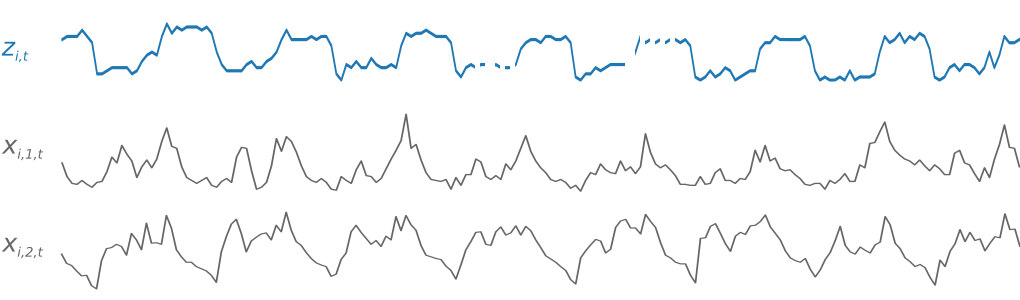
\includegraphics[width=1\textwidth]{images/deepar-explanation.png}
    \caption{DeepAR learns to predict a target (in blue), possibly from dynamic features (in black)}
    \label{fig:deepar-explanation}
\end{figure}


\subsubsection{Use-cases}

The strength of this algorithm resides in the fact that it is able to learn simultaneously from different correlated time series (called \lstinline{targets}) and their associated \lstinline{dynamic features}, which are additionnal time series used as features during training. Please note that it can't be trained on streaming data.

To take a concrete example, let's say we wish to predict the requests hitting the BMW servers on a per-city basis. Our \lstinline{targets} would be the weekly profile of requests coming from each major city, and the associated \lstinline{dynamic features} could for instance be the weekly profile of oil prices and temperatures in those cities.

For the sake of clarity, below is an example of what data shape DeepAR expects. Each line corresponds to a \lstinline{target} time series,  and each \lstinline{dynamic_feat} to a list of its associated dynamic features.


\begin{lstlisting}
{"start": "2009-11-01 00:00:00", "target": [4.3, "NaN", 5.1, ...], "cat": [0, 1], "dynamic_feat": [[1.1, 1.2, 0.5,...]]}
{"start": "2012-01-30 00:00:00", "target": [1.0, -5.0, ...], "cat": [2, 3], "dynamic_feat": [[1.1, 2.05, ...]]}
{"start": "1999-01-30 00:00:00", "target": [2.0, 1.0], "cat": [1, 4], "dynamic_feat": [[1.3, 0.4]]}
\end{lstlisting}

As a further remark, one can point out that DeepAR supports unknown target values during training, which can be useful if we have an outage at some point cutting access to the data stream.

\subsubsection{Behavior on the BMW dataset}

We tried three different approaches with the DeepAR algorithm, all having a common agreement: train on all the dataset but the last week, and test on the last week. \\
It is useful to remark that one could have removed the part of the data being the christmas holidays, but we were curious about the ability of DeepAR to abstract these "outliers". We trained with the following parameters:

\begin{enumerate}
    \item \textbf{Training without dynamic features}
    \begin{enumerate}
        \item[] \textbf{Idea}:\\
        Training set on all data but the last week, performance evaluation on the last week, without any dynamic features.
        \item[] \textbf{Input shape}: \\
        \begin{lstlisting}
        {"start": "2019-11-01 00:00:00", "target": [4.3, "NaN", 5.1, ...]}
        \end{lstlisting}

        \item[] \textbf{Results}:\\
        \begin{figure}[h!]
            \centering
            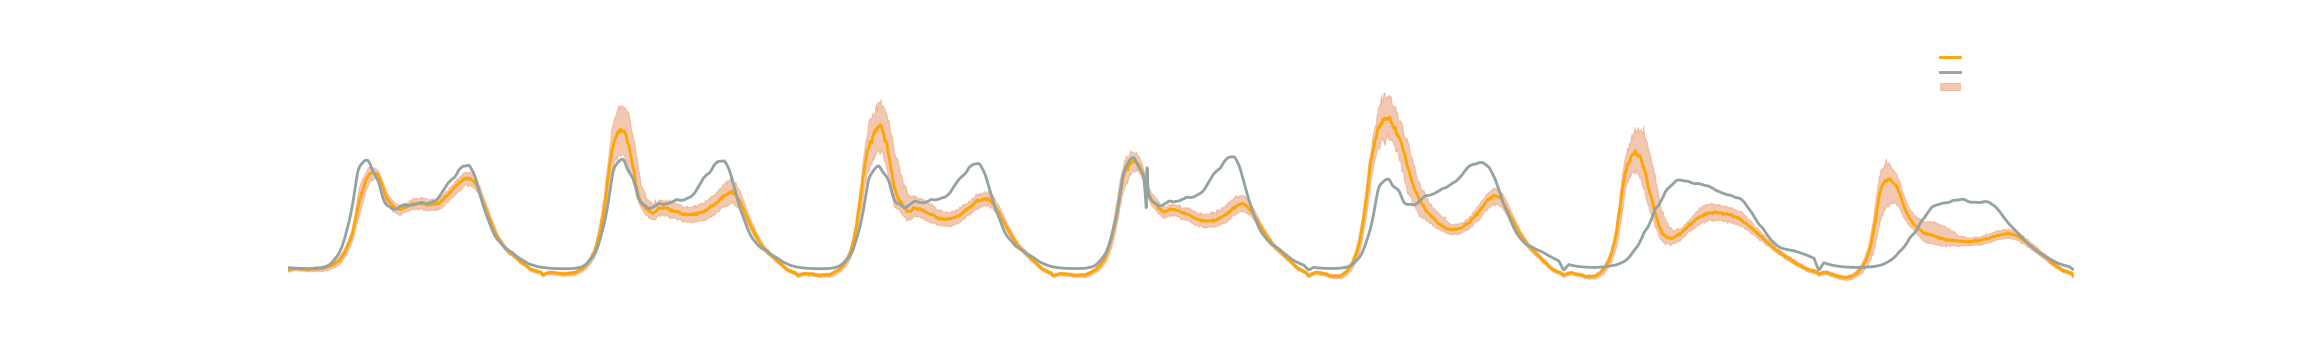
\includegraphics[width=1\textwidth]{images/deepar_no_dyn.png}
            \caption{DeepAR Prediction trained without dynamic features.}
            \description{}
            \label{fig:deepar_no_dyn}
        \end{figure}
        Remarkably, the algorithm performs quite well during the working days with a RMSE (Root Mean Square Error) of 95K. but is unable to learn the trends of weekends. This is quite interesting, since DeepAR is supposed under the hood to automatically encode additional temporal information such as the day of week. Maybe adding some hidden neurons would improve its ability to learn the weekend patterns.
        
    \end{enumerate}
    
    \item \textbf{1-Week forecasting training with holidays features}
    \begin{itemize}
        \item[] \textbf{Idea}:\\
        Training set on all data but the last week, performance evaluation on the last week, with holidays dynamic features. When a day is a holiday, its associated dynamic feature is a one, else 0. \\
        We train the model to predict a full week , with a week of context.
        \item[] \textbf{Input shape}:\\
        \begin{lstlisting}
        {"start": "2019-11-01 00:00:00", "target": [4.3, "NaN", 5.1, ...], "dynamic_feat": [[0, 0, 1,...]]}
        \end{lstlisting}
        \item[] \textbf{Results}:\\
        \textbf{RMSE (Root Mean Square Deviation) of 72K}
    \end{itemize}
    
    \item \textbf{1-Week forecasting training with holidays \& weekends features}
    \begin{itemize}
        \item[] \textbf{Idea}:\\
        Training set on all data but the last week, performance evaluation on the last week, with holidays \& weekends dynamic features. When a day is a holiday, its associated dynamic feature is a one, else 0. And similarly, when a day is a weekend, its associated feature is a one, else 0. We decided to add the weekends feature since in the first part we identified that DeepAR had trouble learning their pattern.\\
        We train the model to predict a full week , with a week of context.

        \item[] \textbf{Input shape}:\\
        \begin{lstlisting}
        {"start": "2019-11-01 00:00:00", "target": [4.3, "NaN", 5.1, ...], "dynamic_feat": [[0, 0, 1,...],[1, 1, 0, 0, ...]}
        \end{lstlisting}

        \item[] \textbf{Results}:\\
        \textbf{RMSE (Root Mean Square Deviation) of 122K }
        Adding the weekends dynamic features deeply worsened the model performance, and we think this is because it might conflict with what DeepAR does already perform under the hood. This shows that adding extra dynamic features do not necessary improve this model.
    \end{itemize}
    

    \item \textbf{3H forecasting training with holidays \& weekends features}
    \begin{itemize}
        \item[] \textbf{Idea}:\\
        Training set on all data but the last week, performance evaluation on the last week, with holidays \& weekends dynamic features. When a day is a holiday, its associated dynamic feature is a one, else 0. And similarly, when a day is a weekend, its associated feature is a one, else 0.  \\
        The main idea behind this is to have a higher hourly granularity during the forecast, this being useful for instance during predictive auto-scaling.
        
        \item[] \textbf{Input shape}:\\
        \begin{lstlisting}
        {"start": "2019-11-01 00:00:00", "target": [4.3, "NaN", 5.1, ...], "dynamic_feat": [[0, 0, 1,...],[1, 1, 0, 0, ...]]}
        \end{lstlisting}
        \item[] \textbf{Results}:\\
        \textbf{RMSE (Root Mean Square Deviation) of 132K}
        For some reason, this tuning of the algorithm did  perform poorly. One of our guess is that the data aggregated in 5-min buckets is too broad, and that we should rather aggregate it in 1-min buckets. Also, it is possible that we are working with too little data as well.
    \end{itemize}
\end{enumerate}


\subsubsection{Discussion and recommendations}

\begin{itemize}
    \item[] As mentionned in AWS description, DeepAR outperforms traditional time series forecasting algorithms when the dataset comprises thousands of correlated time series. We tested it on a single time series coupled with only two dynamic features, but it already had promising results (see \ref{fig:deepar_no_dyn}), improving continuously with the number of dynamic features.
    
    \item[] However, even though DeepAR is supposed to generate additional time features such as day of week, it did not perform well on weekends, and we had to input these features dynamically. This leads us to believe that there is a bit of tweaking to do in order to obtain a foolproof model.
    
    \item[] Due to the lack of geolocalized data, we tested this algorithm on a simple task, whereas it is designed to work on a lot more complex task. Thus, we highly recommend that you try it \textbf{when additional, geolocalized data will be available, such as traffic per world area. In this case, DeepAR could outperform traditional models and give BMW valuable insight}.
\end{itemize} 
    \subsection{Holt-Winter's Method - Marina}
        \textit{Author: Marina Mursa} \\
\label{sec:holt-winter}
An intuitive assumption about the way one can predict the future is that the future should resemble the past experiences. So the most naive approach in forecasting is just to set the position of a future datapoint to the same place as the last observed one. In this section, we will talk in details about an approach that builds on this principal. \\
\subsubsection{Theoretical background}
One of common approaches used for forecasting, that is based on this historical principal, is called \textit{exponential smoothing}. In a simple version of \textit{exponential smoothing} we just copy and paste the last observed data. This however disregards historical data, except for the most recent ones. A more thoughtful approach would be to assign some weight to each data. The more recent a datapoint will be, the bigger its weight value. 

Think about it for a second. Imagine a distribution in the form of a diagonal line, say starting in the bottom left corner going to the upper right corner. Our human perspective can identify easily that the data has a \textit{trend} of going up. If we just average all the datapoints and produce a mean prediction, the prognosis will be a line that goes straight in the middle of the graph. This is obviously not the result we would want.

This way, the simple exponential smoothing can not account for forecasting time series data that has a trend and/or a seasonal component. Luckily, this issue can be resolved by using an upgraded version of smoothing called Holt-Winters method \cite{holt}. 

It divides a time series $Y_{t}$ in three parts: one related to its seasonality ($s_{t}$), one related to its  trend behavior ($b_{t}$) and one for  the residual part ($l_{t}$). For each  of them, a simple EWMA is  applied  to predict a new value.  A  combination  of  these  expressions  is used  to  estimate  $Y_{t+1}$. The following equations represent the HW computation: 
\begin{align*}
  \hat{y}_{t+h|t} &= \ell_{t} + hb_{t} + s_{t+h-m(k+1)} \\
  \ell_{t} &= \alpha(y_{t} - s_{t-m}) + (1 - \alpha)(\ell_{t-1} + b_{t-1})\\
  b_{t} &= \beta^*(\ell_{t} - \ell_{t-1}) + (1 - \beta^*)b_{t-1}\\
  s_{t} &= \gamma (y_{t}-\ell_{t-1}-b_{t-1}) + (1-\gamma)s_{t-m}
\end{align*}
Before explaining how Holt-Winter method was implemented, let's take a moment and think \textit{why would we need to explore this solution}.

\subsubsection{Use-case motivation}
Going back to the use case of this project, the implementation of this algorithm would, in theory, be able to generate a prediction, as well as extract a series of interesting knowledge about historical data.

First of all it would be able to find an existing \textit{trend} in the data. This trend will probably depend on the rate of new cars joining  the ConnectedDrive network over time, or on the growing popularity of certain services (that would increase the number of daily request from a car) and it will be best visible after a large amount of data is collected.

Secondly, it should pick up on any \textit{seasonal components}, if they exist, and give a hint towards existing outside factors that can influence the traffic. A hypothesis can be the fact that in summer, when kids do not have school and lots of people chose to go on vacations, the number of cars on the streets is smaller compared to winter. Once again, having enough data (for at least a year), these type of hypothesis can be tested by training the model and decomposing the data.\\

\subsubsection{Data testing}

To see if such an algorithm is applicable to a dataset, first of all we can run a decomposition function that would try to split a batch of data into the 3 equations mentioned above. 

\begin{lstlisting}[language=Python, caption=Data decomposition]
decompfreq = ((24*60)//5)
sm.tsa.seasonal_decompose(train, freq=decompfreq).plot()
\end{lstlisting}

In figure \ref{fig:holt_winter_decomposition} (Part.1) you can see the results from decomposing the BMW test dataset. If we analyse the graphs, we can observe that the model is doing a fairly good job at handling the data. We purposely included the anomalous first two days (21-22 December) into our training data to observe how well does the model pick up on the existing trend as well as how easy it is to through it off. We can observe that the trends are well preserved, although their specifics are dimmed down.\\
\begin{figure}[h]
    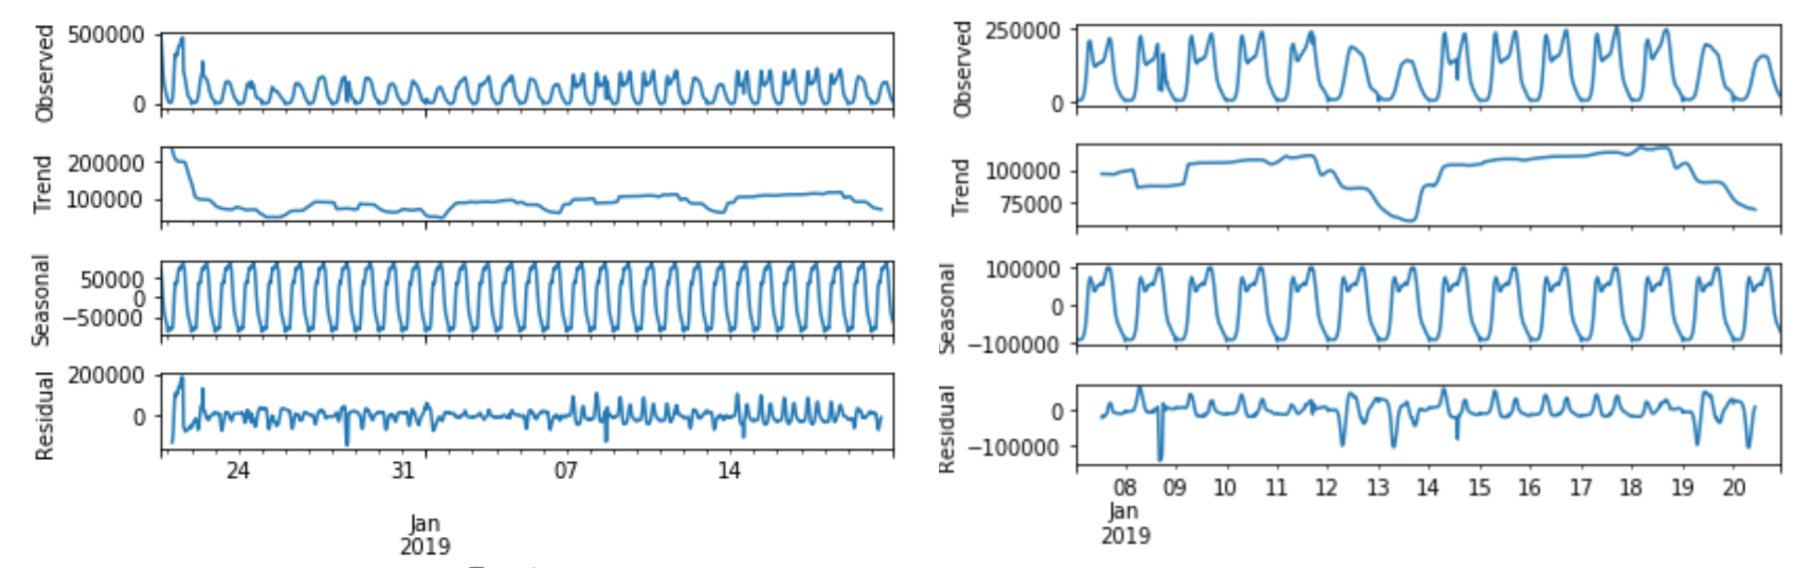
\includegraphics[width=1\textwidth]{images/holt-winter-decomposition.png}
    \caption{Data decomposition into Trend, Seasonality and Residual using Holt-Winter Method }
    \label{fig:holt_winter_decomposition}
\end{figure}
In comparison, the seasonal graph does not do so well, while it does detect a daily pattern, it only plots almost Gaussian distribution of daily data. This is due to the poor quality of data, that includes a holiday period, where the rush hour pattern is non-existent. Another factor that diminishes the pattern is the fact that the model averages over weekends, where again the double-peaked pattern disappears. If we exclude this holiday period, we can see a significant improvement in the pattern (see fig. \ref{fig:holt_winter_decomposition} Part 2).\\

Now that we know that our data is suitable for a Holt-Winter's Method analysis (because it performed the decomposition successfully), let's see how the model can be implemented.

\subsubsection{Model Implementation}
First of all we should go back to our data. The imputed format does not matter much as long as 2 dimensions of the data can be extracted, \verb|count| and \verb|datetime| (or other similar inputs).

Next step is to divided the data into training and test data. As mentioned in the previous sections, the agreement for the prediction algorithms was to leave the last week for testing, otherwise, around 0.2 parts of the data can be left out for model validation.

After having the two sets, no further reprocessing is required.

The \textit{statsmodel} module in Python has a pre-built function to do the so-called \textbf{Triple Exponential Smoothing}. In this method, we can implement both the \textit{additive} and \textit{multiplicative} technique. The additive method is preferred when the seasonal variations are roughly constant through the series, while the multiplicative method is preferred when the seasonal variations are changing proportional to the level of the series.
\begin{lstlisting}[language=Python, caption=Exponential Smoothing method]
    model = ExponentialSmoothing(train, seasonal_periods=seasonl, seasonal='mul').fit()
    pred = model.predict(start=test.index[0], end=test.index[-1])
\end{lstlisting}

The constants \textbf{$\alpha, \beta, \gamma$} (that were mentioned in the formulas presented in the sections above) - can be estimated (usually through a trial and error process known as \textit{fitting}) and can be left for the algorithm to estimate or manually set in the .fit()\footnote{\url{https://www.statsmodels.org/dev/generated/statsmodels.tsa.holtwinters. ExponentialSmoothing.fit.html#statsmodels. tsa.holtwinters.ExponentialSmoothing.fit}} method as following:
\begin{lstlisting}
ExponentialSmoothing.fit(
    smoothing_level=None, smoothing_slope=None, 
    smoothing_seasonal=None, damping_slope=None, 
    optimized=True, use_boxcox=False, 
    remove_bias=False, use_basinhopping=False, 
    start_params=None, initial_level=None, 
    initial_slope=None, use_brute=True
)
\end{lstlisting}
\subsubsection{Results}

Bellow you can see the results of running such an algorithm. Although the \textbf{RSME} is about \textbf{48K}, which is a relatively good performance, and as seen in  fig. \ref{fig:holt_winter_results} the prediction results are close to the reality, they still have the problem of recreating the double peaks pattern. This can be explained by the fact that the algorithm has no means of separating the weekdays from weekends (as DeepAR does), and end up averaging all days together. \\
In addition, because the model puts together three distributions (trend, seasonality and residual) every time it trains, such an algorithm requires a lot of computational power.\\

\begin{figure}[h]
    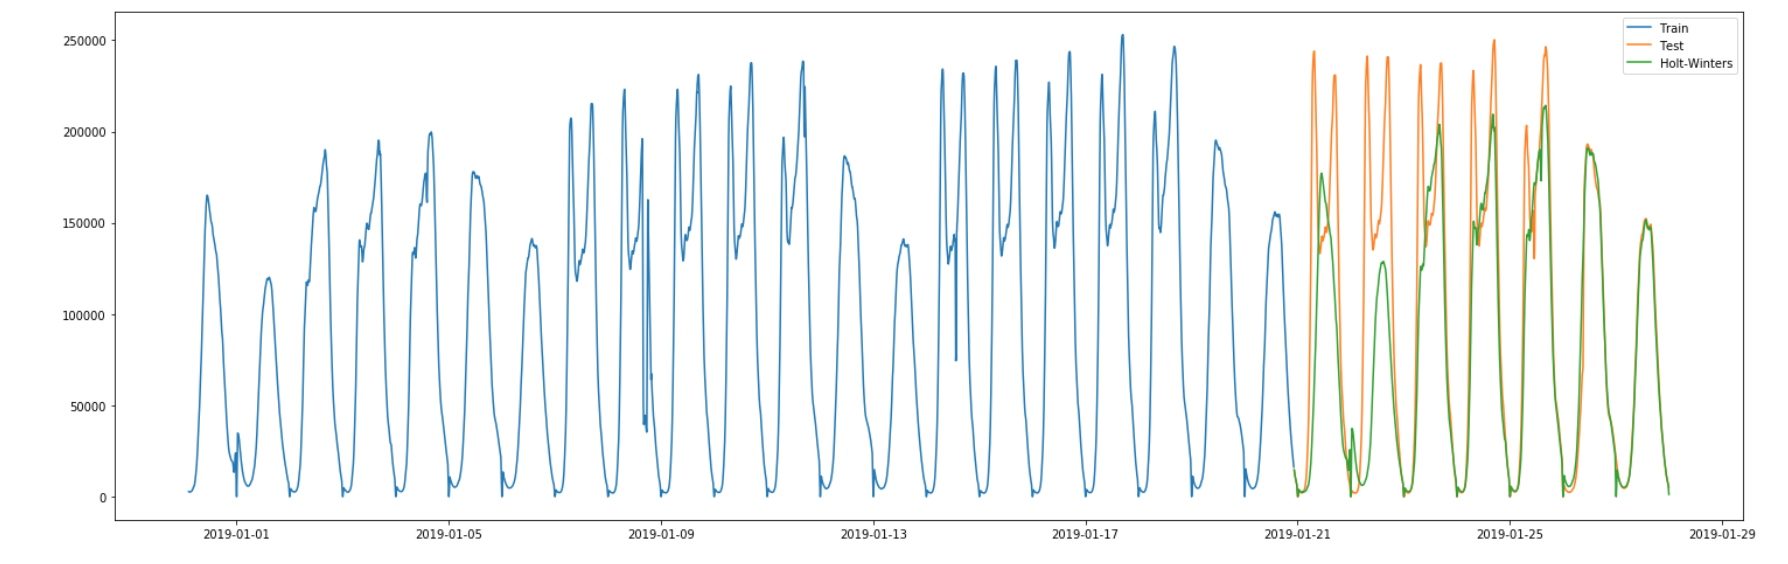
\includegraphics[width=1\textwidth]{images/holt-winter-result.png}
    \caption{Results of Holt-Winter's prediction model}
    \label{fig:holt_winter_results}
\end{figure}

This being said, we need to remember that our motives for trying out this algorithm was to discover new knowledge about data, besides being able to generate predictions. As we saw from the decomposition it only detects the already known day and week pattern. This is of course due to a very small input of data (3 weeks). \\
If we would gather a more considerable amount of training information, let's say for a year, this model would certainly have more secrets to discover.
    \section{Data Management - Ali Jacek}

In the following chapter different ways of connecting the models with the data are described,  as well as what was used to create a work-flow of Data-Model-Results in Notifications.\\

 \subsection{Mean Predictor V1}
 
In this chapter the first prototype of mean predictor will be described. In the pipeline to detect anomalies: lambdas, models, and S3 buckets, to create the work-flow of sending data to a model and retrieving back results, were combined. We had a lot of issues working with lambdas, layers, dependencies and overall usage of a single lambda across several users. 

A great challenge was discovering usage of layers. Tool that enables easy possibility of importing several additional python libraries to a lambdas. Thanks to the layers, lambdas development process can be accelerated and shared among other developers. AWS built in libraries no longer limit us and lambdas code can be viewed in the AWS console.  Layers even though they are very powerful are badly documented and it took us a great deal of time to discover the correct usage. 

Mean Predictor was a simple model we first created, and the lambdas used to make it fully functional revolved around accessing an S3 bucket with the correct permissions and policies, retrieving data or modifying data in said bucket, then sending it to the model. Input data format is json and the results where either json or in CSV format, according to our needs we changed the formats on demand. 

Two main functions where used here, \verb|Model\_Data\_Join.p| and \verb|AnomalyDetection.py|. We also used a function \verb|alertDemo.js| for slack integration and alerts. Our first phase of testing how can we connect all of these together took a while, but we managed to make it work. Each function of those used different policies and dependencies, and AWS has some limitations with uploading .zip files larger than a specific size. We also created Layers, acting like a placeholder for all dependencies that are being used. In addition to those, we also made an API Gate-Away named \verb|RCF\_Data\_Join\_SageMaker| that gives us the possibility to call the model and send some data to it, without actually being in AWS console at all. We used PostMan for the requests. Our plans where to create simple web-page that you can upload a data file to it, and gives back the result instantly.

\begin{figure}[h!]
    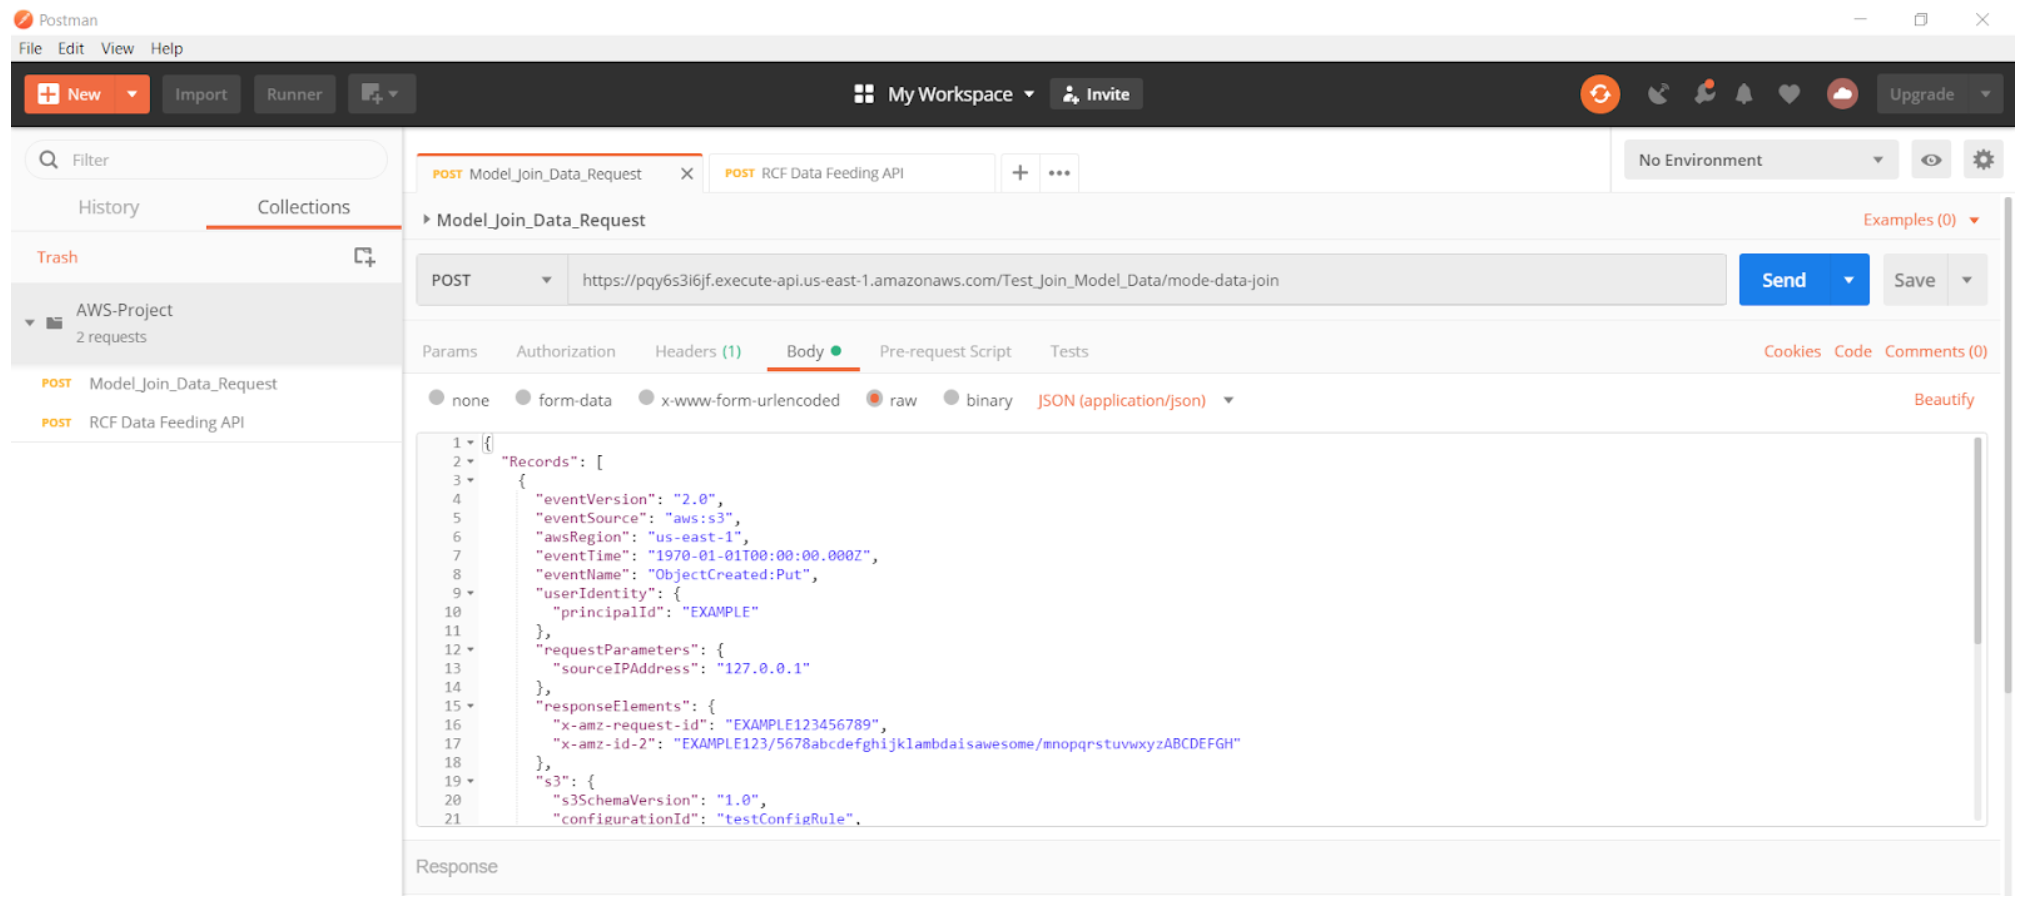
\includegraphics[width=1\textwidth]{images/api-gateway.png}
    \caption{Example of API Gateway using Postman}
    \label{fig:api_gateway}
\end{figure}

\textbf{Model\_Data\_Join.py} can be found in the \verb|/lambdas| folder in the github repository.
This function main job is sending data to the model. Using a specific prefix directory, we let the function access our data bucket and look up all keys inside it. The sent data is going to be tested for anomalies, so we couldn't just send a VPC-FlowLog to the model. Instead, we created a file reader, where we read all the keys inside the directory (Keys are FlowLogs), we parse a small json file with index + number of lines inside them. Number of lines = number of request inside each single Flowlog. This was the most convenient way to send requests number to the model using FlowLogs (Fig. \ref{fig:lambda_key_reader}).

\begin{figure}[h!]
    \centering
    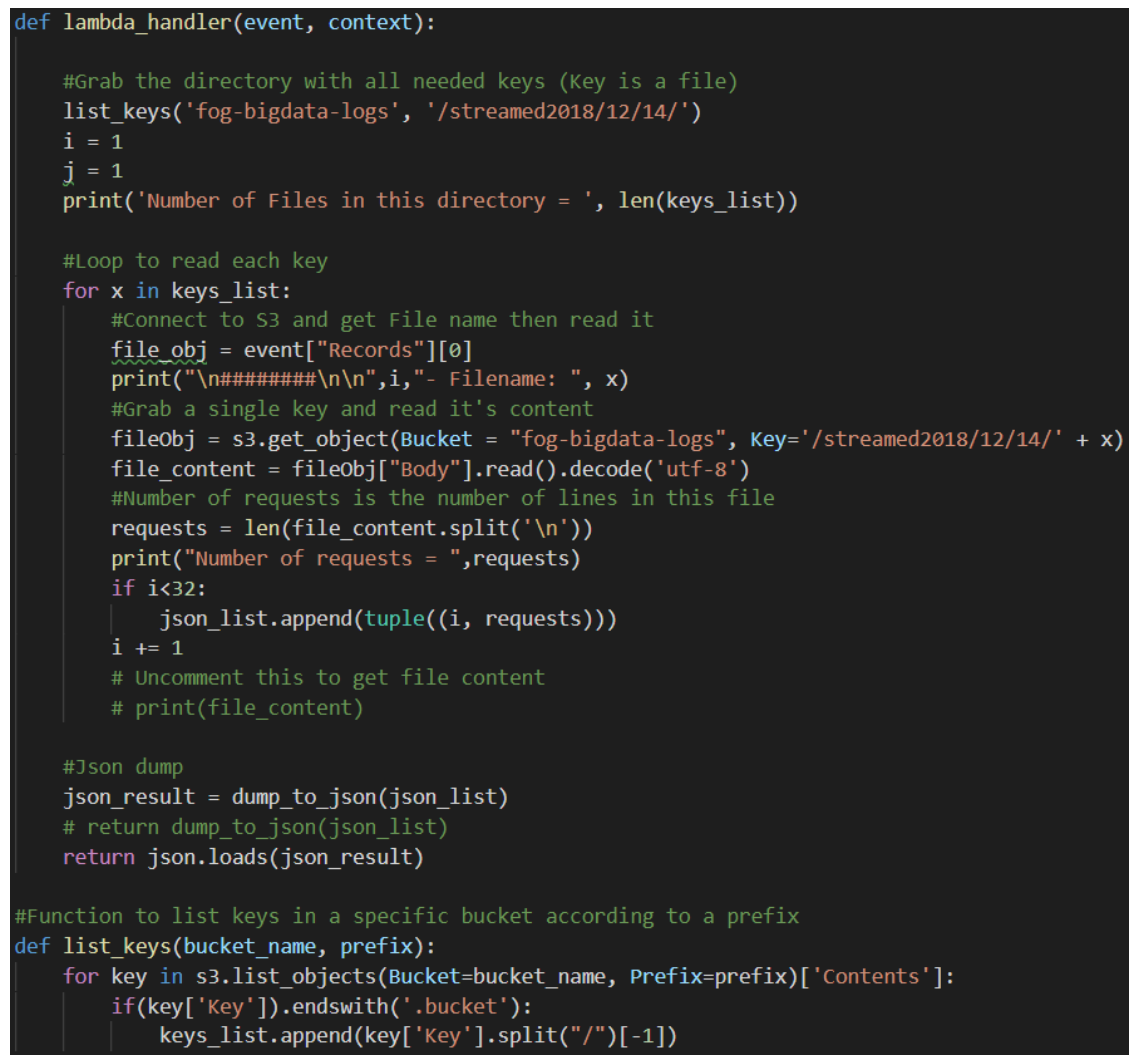
\includegraphics[width=1\textwidth]{images/lambda-key-reader.png}
    \caption{Lambda Key Reader}
    \label{fig:lambda_key_reader}
\end{figure}

After the data has been parsed from the keys, we get a list, converted to a JSON file later dumped inside the bucket to keep as a history of data that has been used. 
This process also involves sending the data to the model, after parsing it to json format. We used the invoke method provided from AWS to achieve this. The method takes another lambda function \verb|AnomalyDetection| and the data file as a variable \verb|(json\_data)|. Below you can see the code for this.

\begin{figure}[h!]
    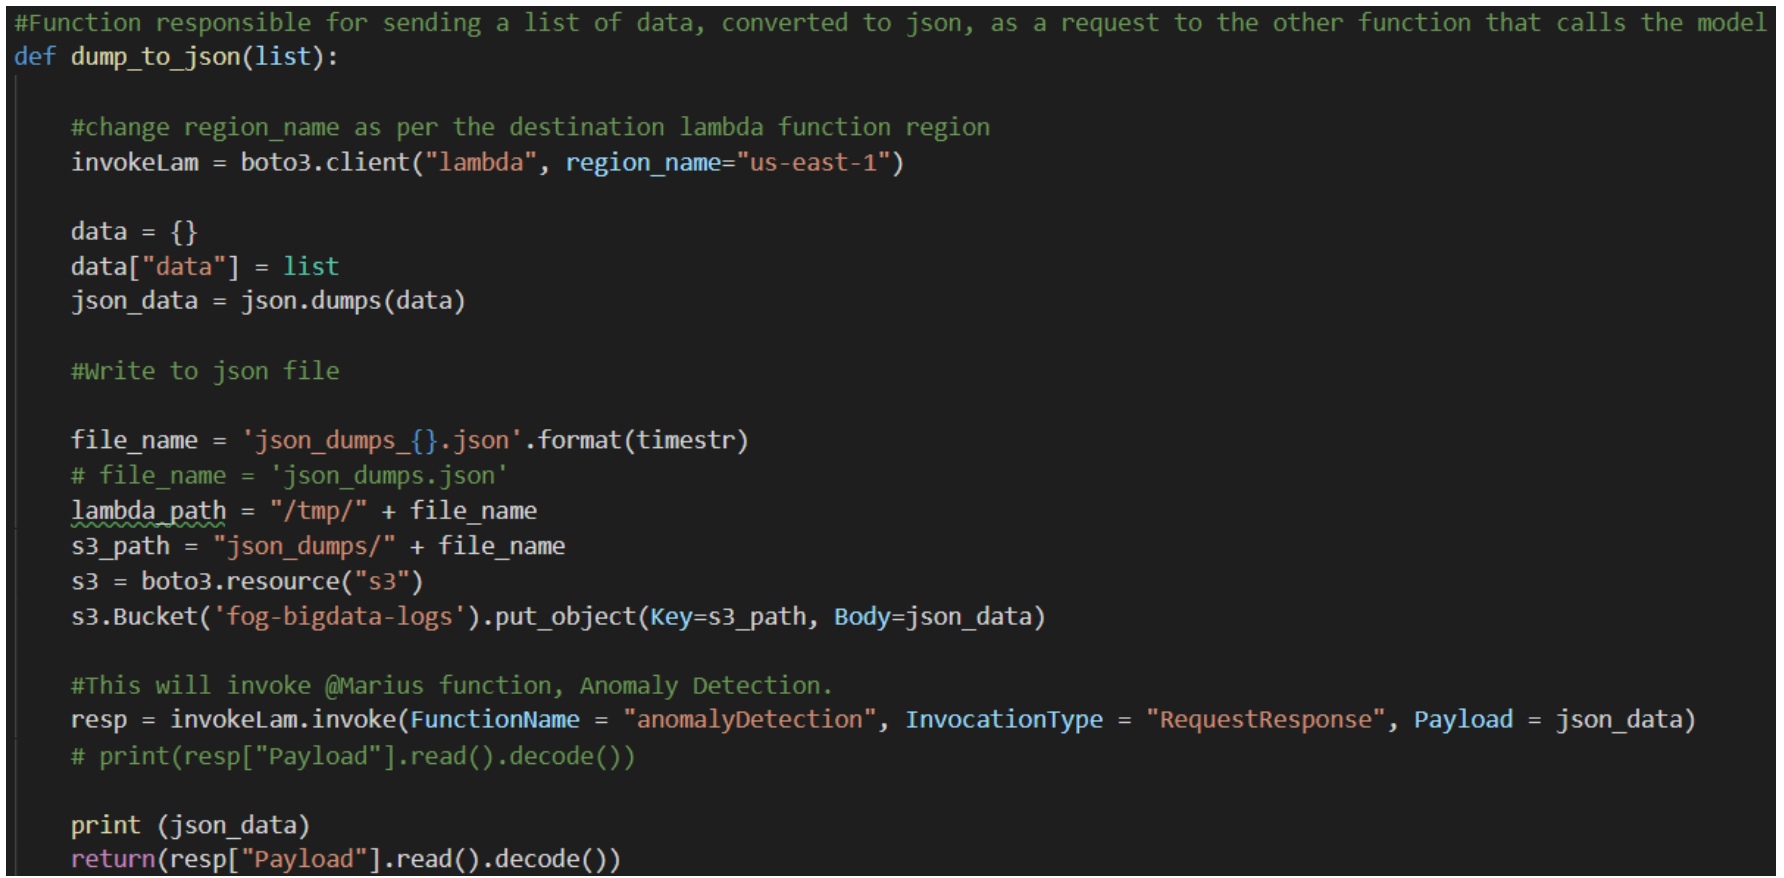
\includegraphics[width=1\textwidth]{images/json-dump-code.png}
    \caption{JSON Dump code}
    \label{fig:json_dump_code}
\end{figure}

After sending the data to \verb|anomalyDetection| lambda, we parse the event back to CSV format for the model to understand it. We separate each value by a new line. Result from the model is then parsed and passed through a prediction method to give us which values where TRUE as anomalies. This result is sent to our AWS channel using an SNS topic (arn:aws:sns:us-east-1:746022503515:api-test) created to queue all notifications.
\begin{figure}[h]
    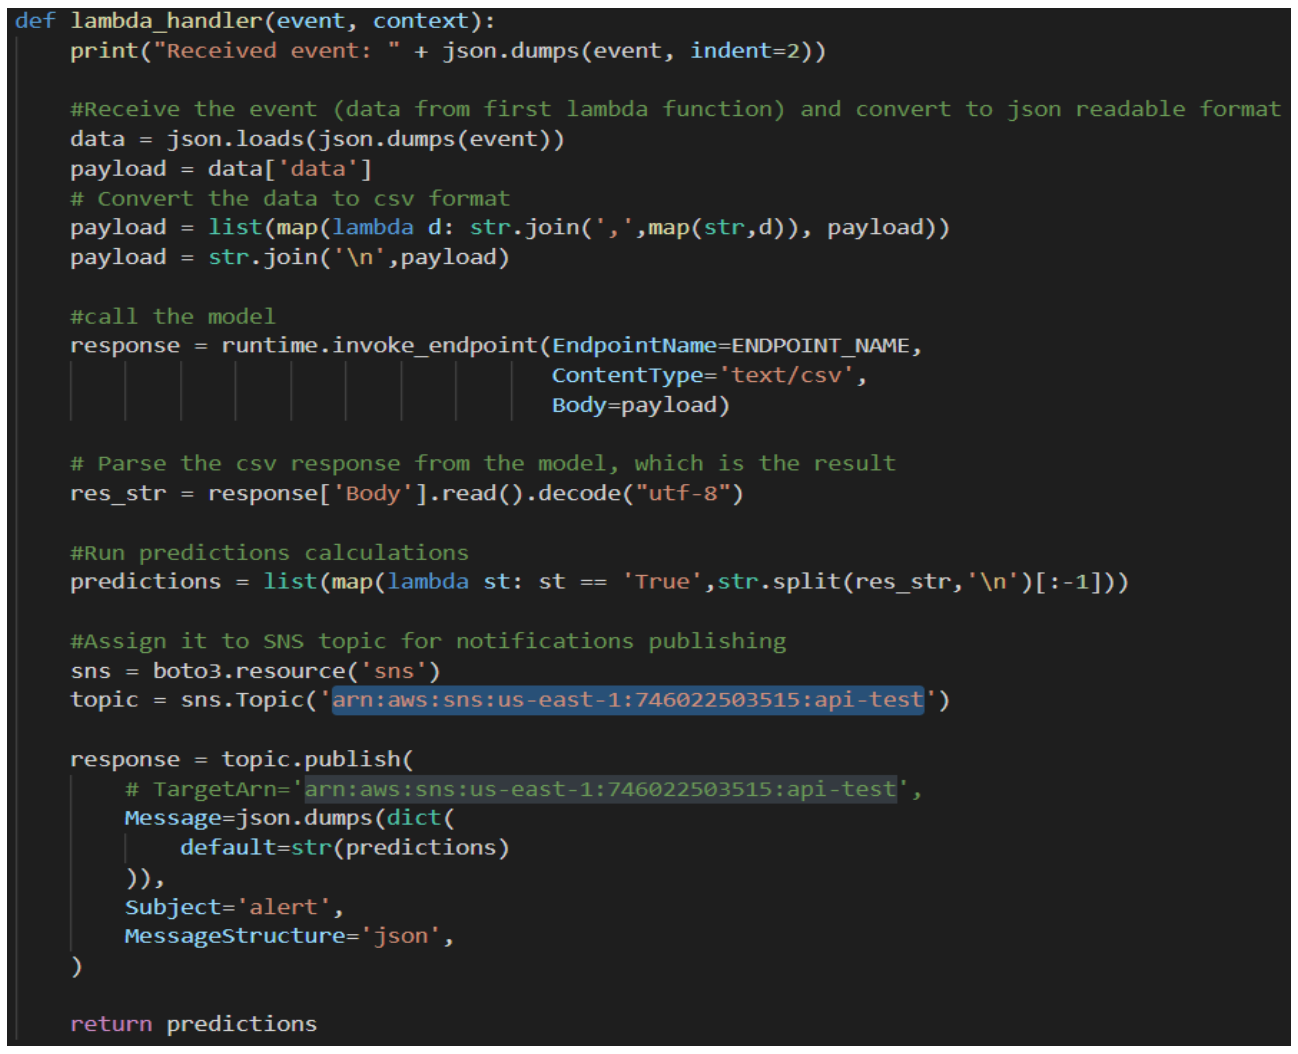
\includegraphics[width=1\textwidth]{images/lambda-precistion.png}
    \caption{Lambda precision}
    \label{fig:lambda_precision}
\end{figure}
Since this was our first demo, we didn't enable automatic triggering with every new data file, instead, we created test events with the needed buckets and triggered them manually. To make it work properly, you just need Flow-Logs inside the directory (as shown in Fig. \ref{fig:lambda_precision}). 
            

\subsection{RCF (Fixed Data)}
RCF Random Cut Forest is unsupervised algorithm for detecting anomalous data points within a dataset and was used in a SageMaker as our second trial model. \\

The data connection with this model was a bit more complex; even though the model took normal json format, we had to separate the values and parse the results several times to make a clean execution. The model takes a list of data points, then returns back a result which is \verb|Scores\_Array|. These scores have to be calculated again using a specific function to get the anomalies (above or below the RCF threshold). Based on those values, we trigger an alert that sends notifications to our channels. However, the procedure also was changed to almost fully automatic! We added a trigger to the functions \verb|rcf-sagemaker-testdata| with a suffix (.csv) and objectCreated event over an S3 bucket, which triggers the whole work-flow by itself. An API gateway \verb|RCF\_API| was also created for the same purpose of our first model.\\

Two S3 buckets were involved in this process, \verb|rcf-sagemaker-finished| and \verb|rcf-sagemaker-testdata|. A small overview of the work-flow is described below:
\begin{enumerate}
\item Make sure the model endpoint is working properly (preliminary checks per usual)
\item Upload data to 1 bucket \verb|rcf-sagemaker-testdata|
\item This upload to S3 bucket automatically triggers using SNS topic all subscribed lambda functions.
\item 2 functions are then triggered. The data from S3 bucket is read, prepared and send to the model. Since the model is already feed with a new data, the input data from the initial S3 bucket are moved to the finished sets to \verb|rcf-sagemaker-finished| S3 bucket.
\item Results and especially the anomaly detection, trigger the notification functions which inform the user about the anomalies.
\end{enumerate}

\textbf{Used functions}
The whole process involved 2 functions, \verb|RCF\_Data\_Join\_SageMaker.py| and \verb|RCF\_Anomaly\_Model\_2.py|. The first function is triggered by file upload to the S3 bucket and reads uploaded data. After parsing the data the function sends the filtered data to the second function, where we call the model for analysis.
All policies, notes, used variables, endpoint names etc. can be found in github repository under \verb|Notes.txt|.
The function reads all files in the S3 bucket and lists them for logging purposes. Once we upload a file, it separates it into 2 versions. The data is usually DATE SCORE format.
So we create 2 lists, 1 with both values and 1 that has only the scores data. We do this because we want to preserve the date as time-stamp history for the model.
Once we have the parsed data, the process of sending this data starts. The smart thing about this is that we used AWS functions to clear our buckets. The data gets sent from \verb|rcf-sagemaker-testdata| bucket to \verb|rcf-sagemaker-finished| bucket, with the name changed to include time of the data testing and date as shown in the Fig. \ref{fig:rcf_data_movement}.\\

\begin{figure}[h]
    \centering
    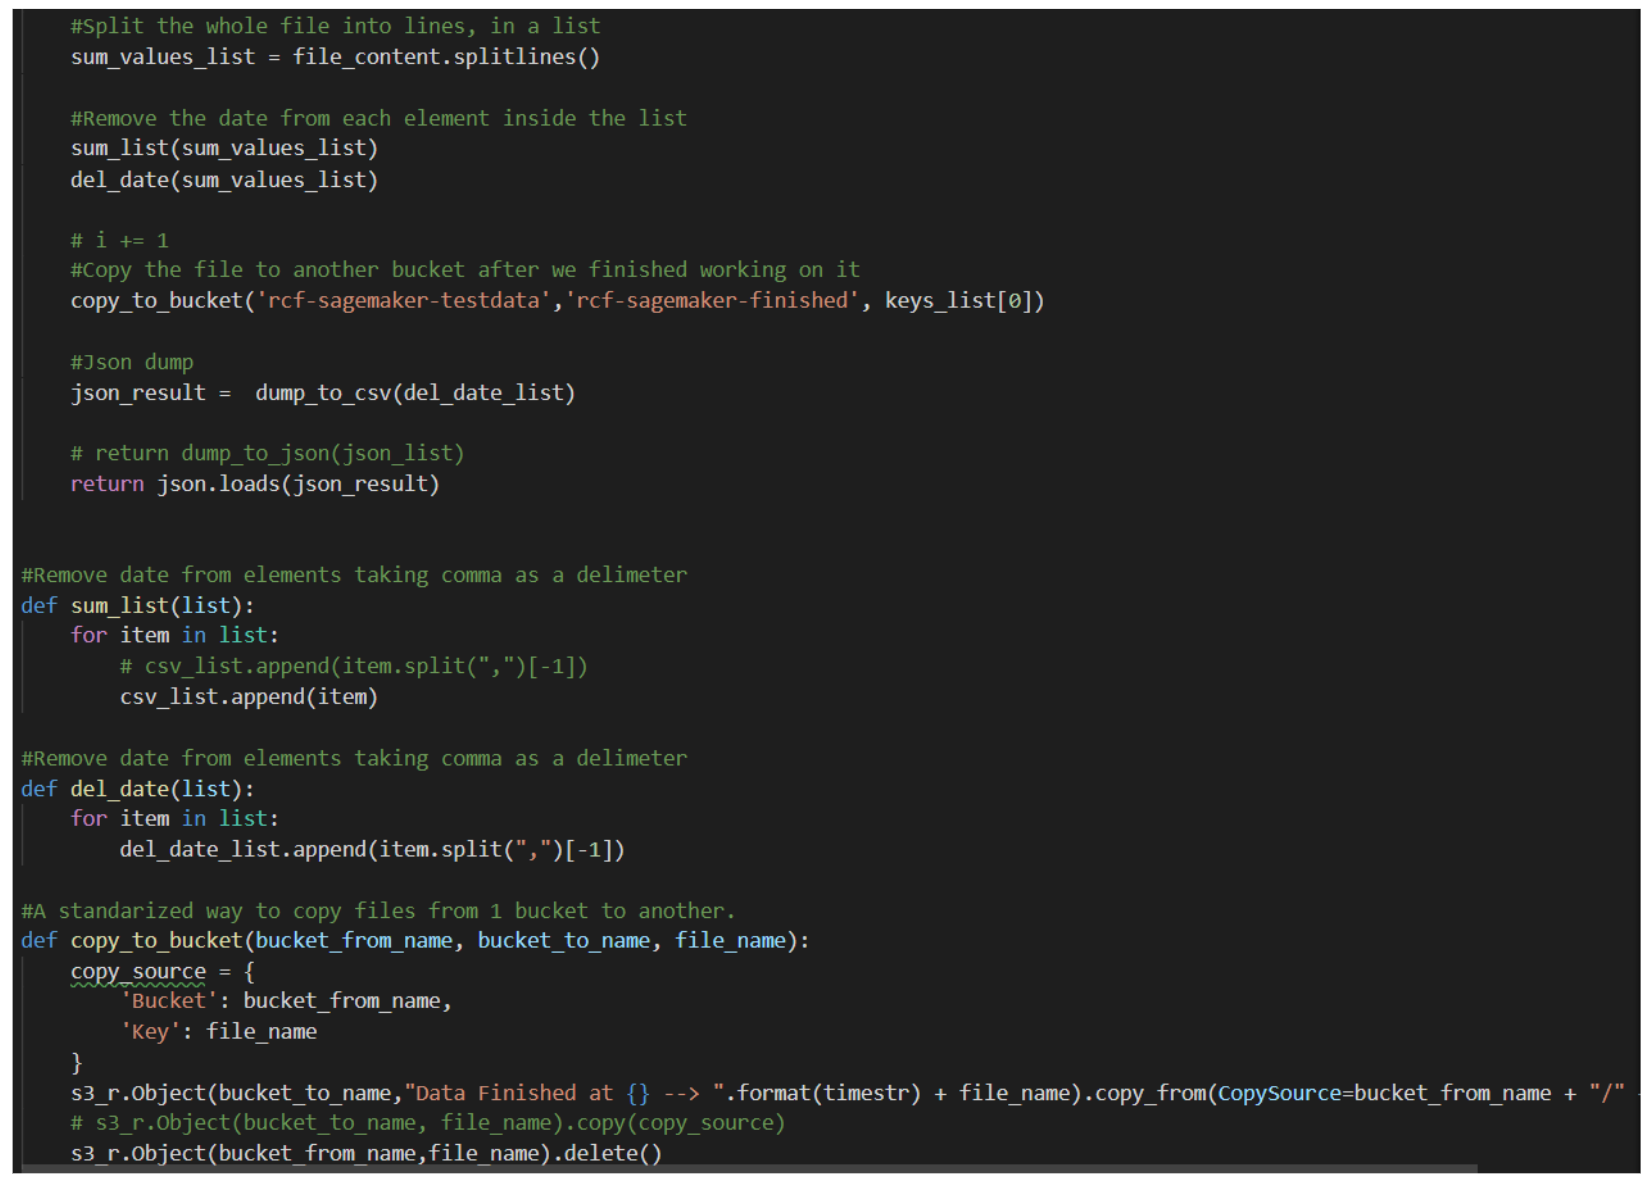
\includegraphics[width=1\textwidth]{images/rcf-data-movement.png}
    \caption{The moving of data from testing buckets to finished testing data}
    \label{fig:rcf_data_movement}
\end{figure}

We then proceed to call \verb|dump\_to\_csv|, where we send the data to the model including the date time-stamp, and also create a \verb|csv\_dump| folder inside the finished bucket for testing and debugging purposes.\\

The model function, \verb|RCF\_Anomly\_Model\_2.py| is then invoked with the needed json data. 
\begin{figure}[h]

    \centering
    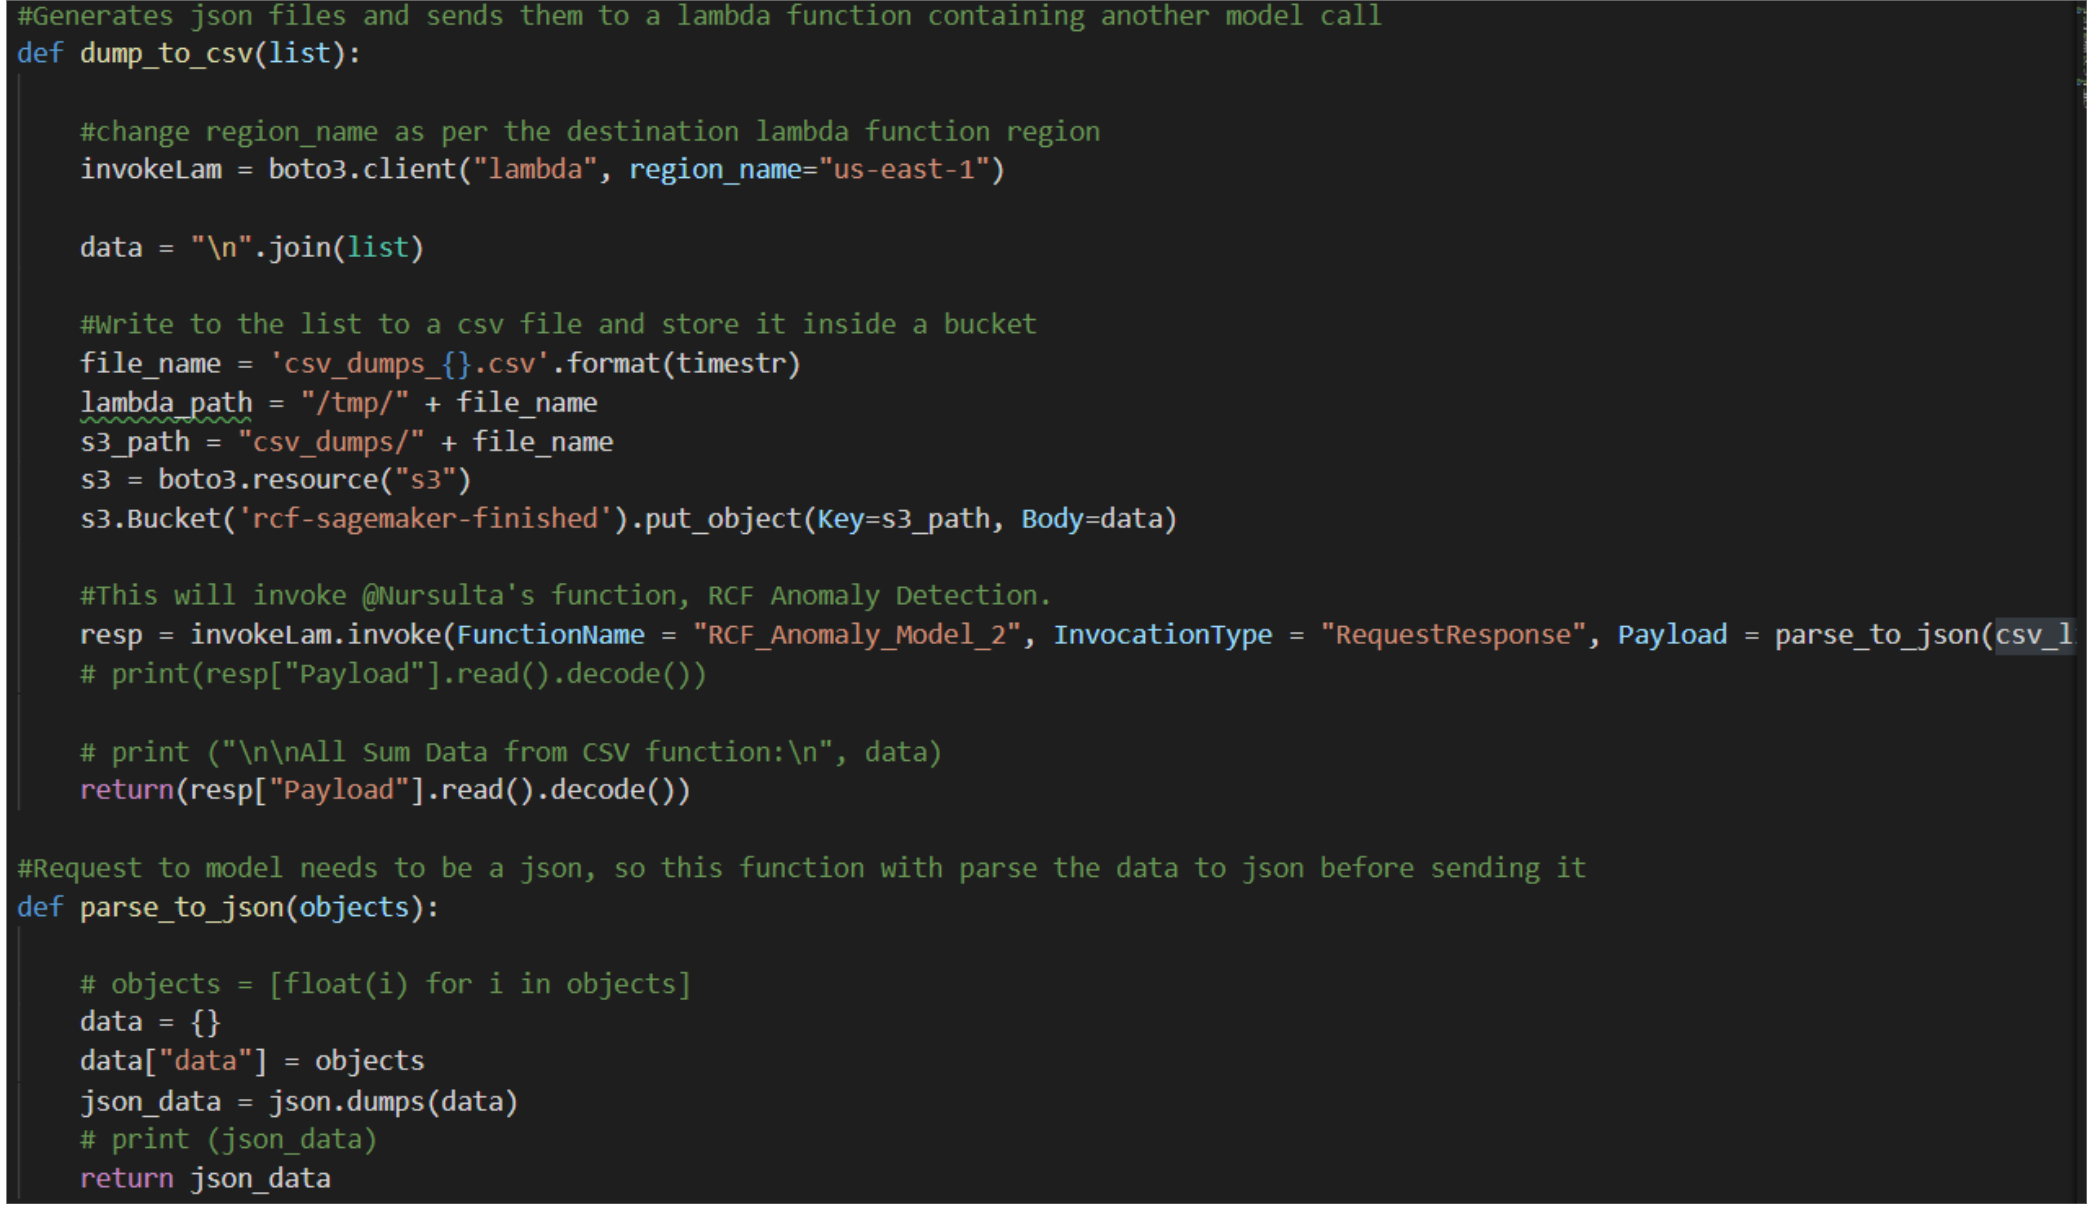
\includegraphics[width=1\textwidth]{images/json-generator.png}
    \caption{Invoking RCF-Anomly-Model-2.py}
    \label{fig:json_generator}
\end{figure}
And as a result of some time consuming calculations in this function, we had to make the run-time of lambda up to 3 minutes to avoid any unwanted failures.\\
After the json event is received, we parse it back to the correct csv format and send it to the model using \verb|invoke\_endpoint| method. The result is a huge CSV response with all the values we need to calculate with RCF for anomalies.\\
The final cut-off score is calculated with the following equations:
\begin{figure}[h]
    \centering
    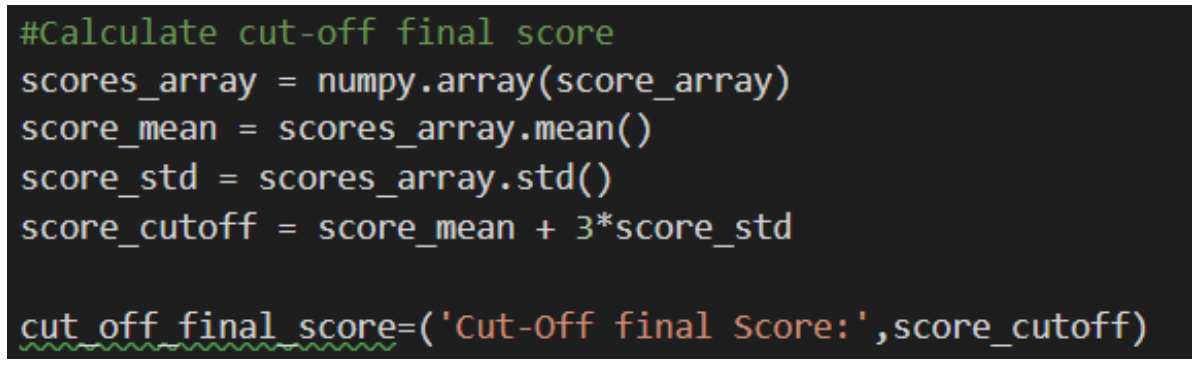
\includegraphics[width=1\textwidth]{images/cutt-off-calculator.png}
    \caption{Cut-off score calculator}
    \label{fig:cut_off_calculator}
\end{figure}
Based on the calculated RCF Threshold we compare the values based on the input data and mark those over the threshold level as an anomalies. Once anomaly is detected notification process starts.\\
\begin{figure}[ht]
    \centering
    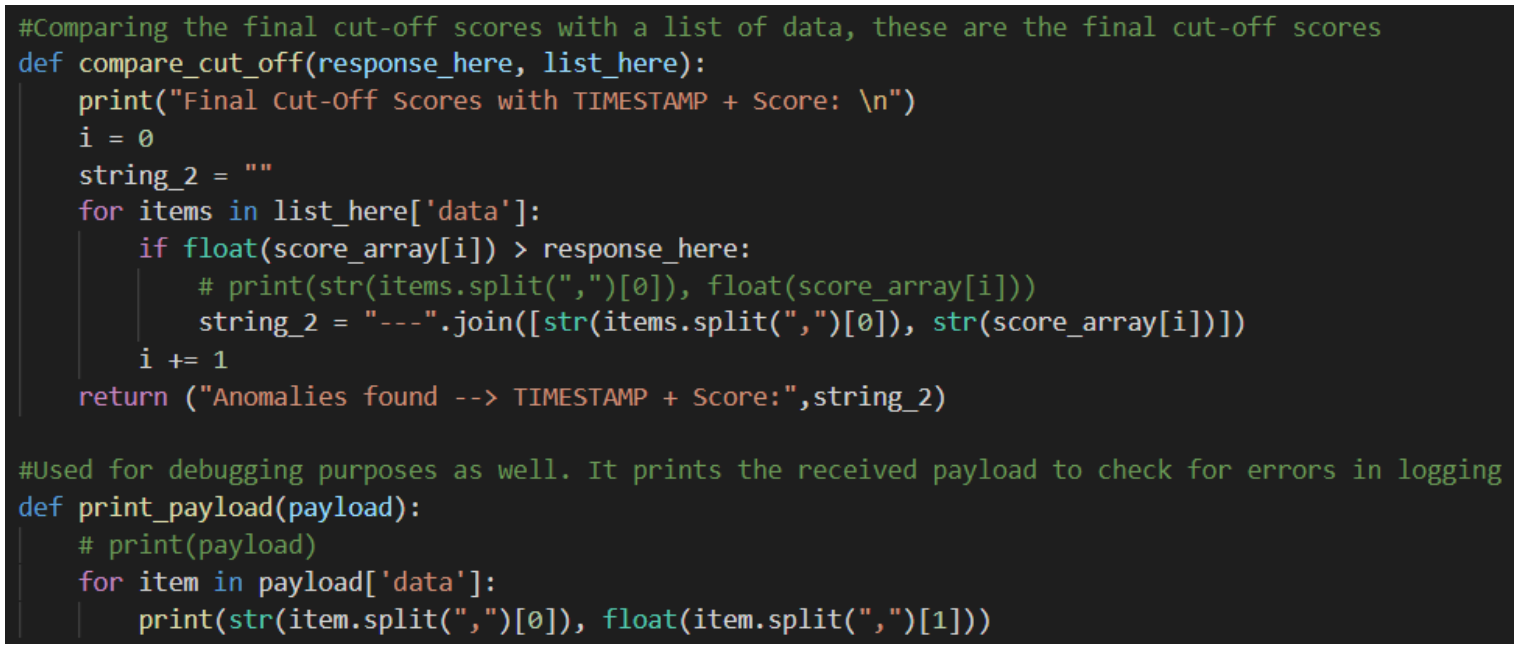
\includegraphics[width=1\textwidth]{images/cutt-off-comparison.png}
    \caption{Cut-off comparison}
    \label{fig:cut_off_comparison}
\end{figure}
Once we have everything calculated and compared, the results are sent to another part of the function where we start sending alerts and notifications. For this we created a specific Slack App \& another function that handles all the notifications. This can be found in a detailed section down below under Notifications Functions.\\

The graph generation was a bit of a complicated manner, since we can’t send direct images from lambda to slack without doing a workaround. We had to store the results in a memory buffer, and read that buffer to send it. Notifications being sent had the anomalies, a graph with the data + threshold + anomalies detected in a detailed form.\\

Using panda, we saved data points in an X (\textbf{Date Stamp}) and Y (\textbf{Scores}) lists after reading the file from lambda’s tmp directory and generate the plot.
\begin{figure}[h]
    \centering
    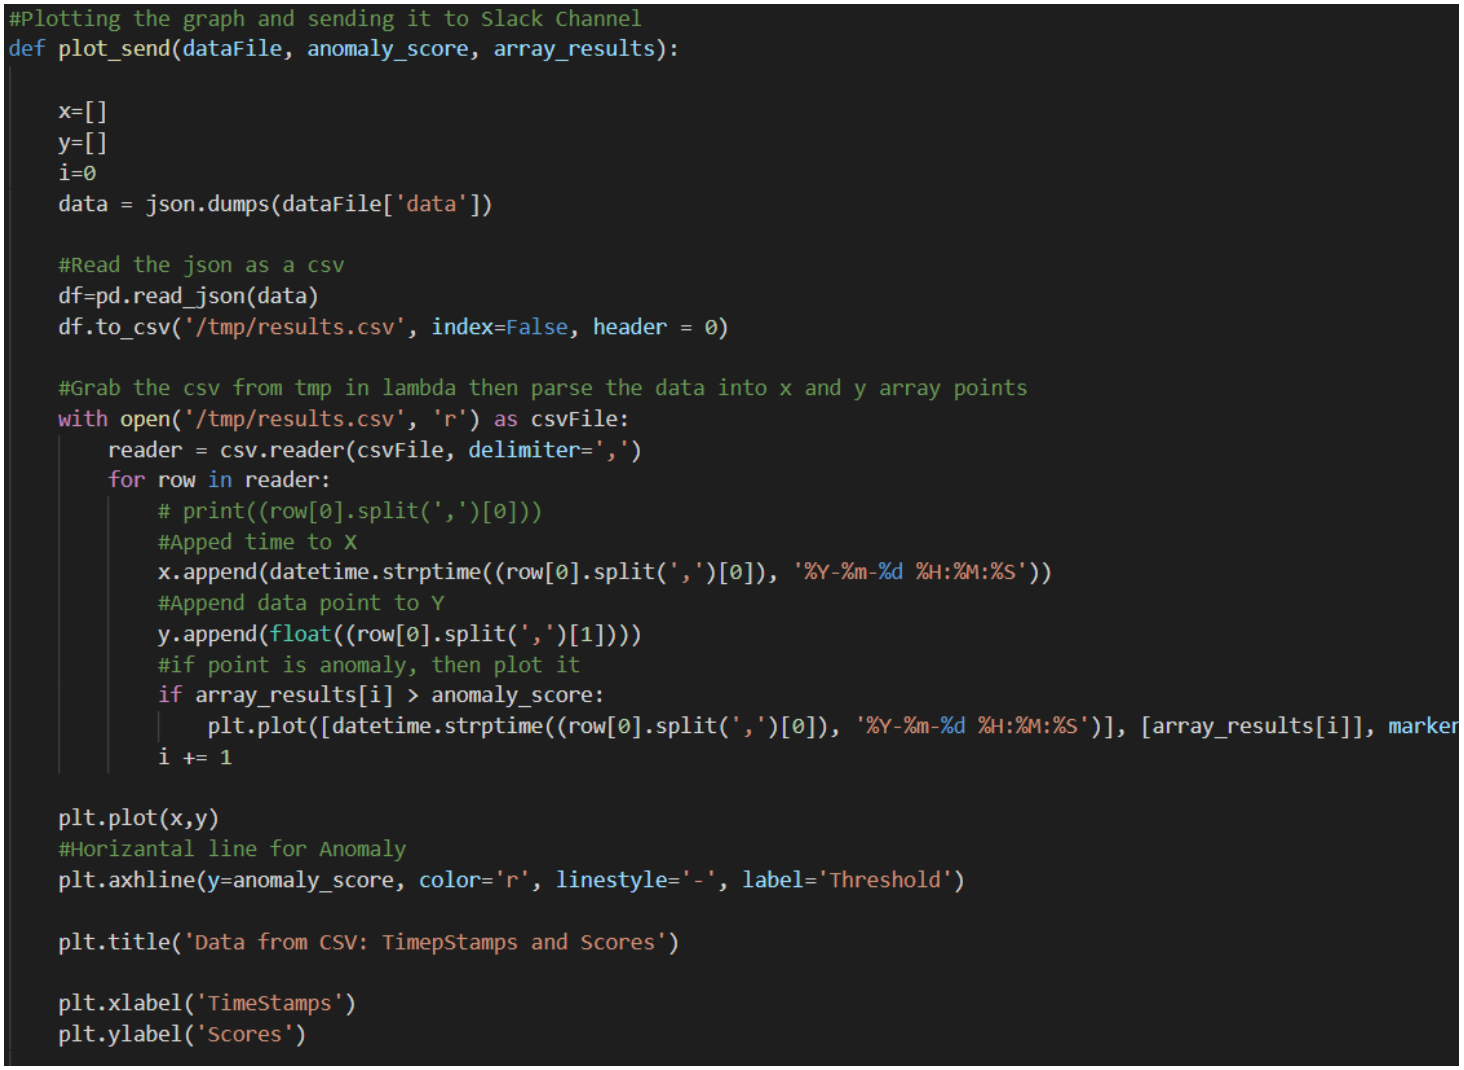
\includegraphics[width=1\textwidth]{images/graph-plotting.png}
    \caption{Plotting the anomaly graph}
    \label{fig:graph_plotting}
\end{figure}
Then sent to slack with a special \verb|payload\_2 param|, that holds our channel name, title and some other needed variables for better readability. In general, this all happens in an automatic form.
    \section{Notification functions - Jacek}

Notification part is a very important part of our project. After collecting the data, preparing them and using machine learning algorithms, we need to somehow communicate with the user. In this paragraph we will describe the motivation and ways of informing the user about the anomalies and predictions.

\subsection{Motivation}
To notify the user in order to react for the main events such as anomaly detection, we created a notification functions. Firstly we are calling user by triggering ChatBot API and secondly we are sending notification to the slack channel with a graph and marked anomaly to let user faster react for it.

\textbf{User story} \\
We decided to create a user story where user who will be notified in case of an alert is one of the administrators Bob. Bob and his team are using slack in their work as we do in this project. \\
In case of the anomaly detection we are triggering ChatBot API to call Bob and notify him about the anomaly. To let Bob faster make his decision and in case of emergency, escalate the problem(or in case of false detection skip it), we decided to show to him the graph where he can visually asses the problem. Since Bob and his team are using slack we decided to send them notification to special slack channel as well. \\
To accelerate the decision making process, even before logging in to the consoles, cloud watches etc. we decided to send him a part of the graph with prediction and marked anomaly. This will be straightforward information for the Bob or his colleagues what is happening. The example of notification massages send to the slack channel is depicted in a fig. \ref{fig:userNotif}.

\begin{figure}[h!]
    \centering
    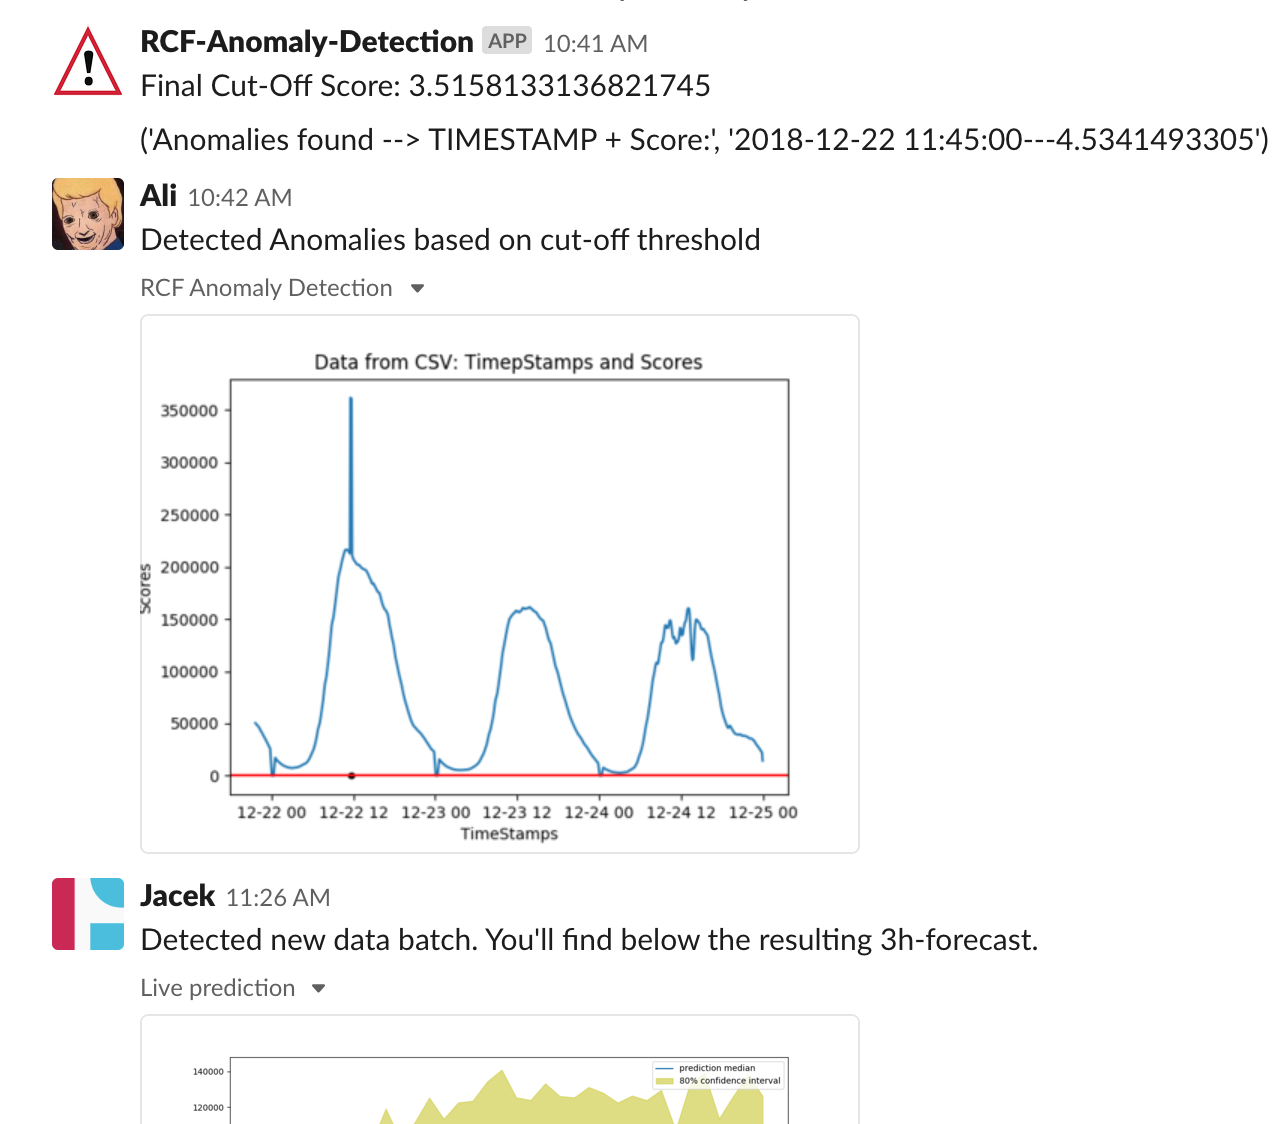
\includegraphics[width=0.8\textwidth]{images/UserNotification.png}
    \caption{Example of anomaly notification}
    \label{fig:userNotif}
\end{figure}

\subsection{Methods to notify the user about detected anomalies}
\begin{itemize}
\item \textbf{ChatBot API notification} - To notify the ChatBot API in case of an anomaly we are sending REST POST message to provided by ChatBot team URL as it is shown in an example in fig. \ref{fig:chatbot}. That POST is triggering ChatBot which calls the user.
\end{itemize}

\begin{figure}[h!]
    \centering
    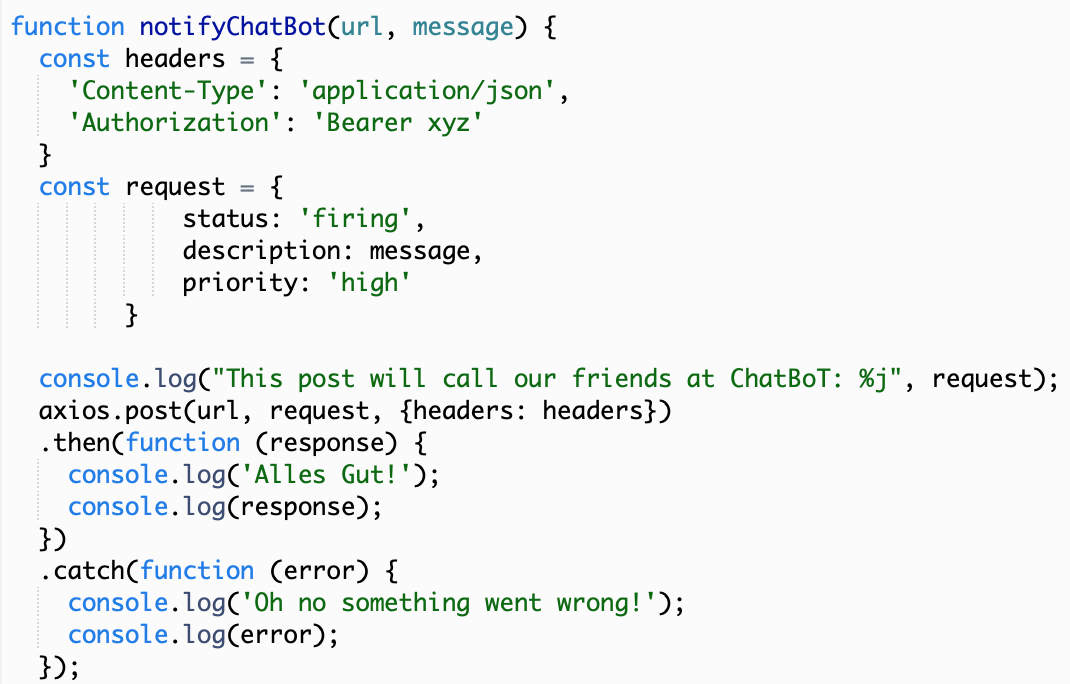
\includegraphics[width=0.85\textwidth]{images/chatbot-api-notif.png}
    \caption{Example of ChatBot API notification}
    \label{fig:chatbot}
\end{figure}


\begin{itemize}
\item \textbf{Slack channel metrics} - To send the message with exact metrics and data we are sending the message to the slack channel using Amazon Simple Notification Service topic.

\begin{lstlisting}[language=Python, caption=Sending message to slack channel using SNS topic]
    #Send Slack MSG
    sns = boto3.resource('sns')
    topic = sns.Topic('arn:aws:sns:us-east-1:746022503515:RCF-SageMaker')
    
    response = topic.publish(
        Message=str("Final Cut-Off Score: {}".format(score_cutoff)),
        Subject='#aws',
        MessageStructure='text/plain',
    )
\end{lstlisting}
\item \textbf{Slack channel graph} - Unfortunately to send the graph to the slack channel method with using SNS topic was not working correctly. For showing the graph using AWS lambda function we needed to do the following steps:

\begin{enumerate}
\item Plot a new graph in memory.
\item Save that graph to a buffer and go to the beginning of a buffer
\begin{lstlisting}[language=Python, numbers=none]
    buf = io.BytesIO()
    plt.savefig(buf, format='png')
    buf.seek(0)
\end{lstlisting}
\item Add a buffer to a structure
\begin{lstlisting}[language=Python, numbers=none]
    my_file = {
    'file' : ('./buf.jpg', buf, 'png')}
\end{lstlisting}

\item Add that structure to the REST POST and post that file to a slack channel.

\begin{lstlisting}[language=Python, numbers=none]
    r = requests.post("https://slack.com/api/files.upload", params=payload, files=my_file)
\end{lstlisting}

\end{enumerate}
\end{itemize}




% Amazon Simple Notification Service - to notify the easiest way.

    \section{Project delivery - Alex}

After six months of intensive work, we ended up with a pretty diverse code base that we needed to unify. We had various models, lambda functions, EC2 instances, roles and policies composing our processing pipeline, and hand them in the most convenient way.

\subsection{Terraform}

\textbf{The source code for this part is located in \lstinline{terraform/}.}\\
We chose to use the infrastructure-as-code deployment tool \href{https://www.terraform.io/}{Terraform}, with a few quirks that are presented below. \\
Terraform uses a \lstinline{state} to keep track of the state of managed cloud components, and perform its changes. This file is created locally on the machine running the terraform commands, but problems arise when two or more people try to concurrently run terraform scripts at the same time : inconstistencies could arise from such situations, which is to avoid at all costs.\\
To deal with this problem, we added the following piece of code: 
\begin{lstlisting}

 terraform {
  backend "s3" {
    bucket         = "fog-bigdata-terraform-backend"
    dynamodb_table = "terraform-state-lock-dynamo"
    key            = "backend/terraform.tfstate"
    region         = "${var.region}"
    encrypt = true
  }
} 
\end{lstlisting}

Which hosts this \lstinline{state} in a remote s3 bucket, allowing thanks to a locking mechanisme several people to work concurrently on the terraform files.

\subsection{Lambda functions deployment}
AWS has recently released a lambda function management tool called \href{https://docs.aws.amazon.com/serverless-application-model/latest/developerguide/what-is-sam.html}{SAM}, but unfortunately Terraform does not support it yet, so we had to package our lambda functions in ZIP files (\href{https://docs.aws.amazon.com/lambda/latest/dg/lambda-python-how-to-create-deployment-package.html#python-package-dependencies}{ref}) and use Terraform's \lstinline{aws_lambda_function} to deploy them.

We had to overcome some hurdles, which are built-in AWS limitations regarding lambda functions: 
\begin{itemize}
    \item Zipped deployment package size limited to 50MB
    \item Unzipped deployment package, including layers, limited to 250MB
\end{itemize}
Since we are using the Matplotlib and Pandas librairies, we ended up with deployment packages weighting more than the AWS limit. \\
That's why we came up with the idea of creating our own layers (thanks to \lstinline{aws_lambda_layer_version}), and linking our lambda functions to those layers. Thus, we end up with ligthweight lambda functions ( \< 1MB ), and also reusable layers.

\subsection{IAM roles and policies}
Every AWS service needs the correct policies to access the other components it works with. For instance, our lambda functions need to access AWS S3 and AWS SageMaker, and this is fortunately well supported by terraform.\\
The code below creates:
\begin{itemize}
    \item A role that can only be assumed by AWS Lambda services
    \item Two policies giving full access to S3 and Sagemaker, attached to this previous role.
\end{itemize}

\begin{lstlisting}
resource "aws_iam_role" "lambda_sm_s3_role" {
  description="Role giving lambda full access to S3 and SageMaker"
  assume_role_policy = <<EOF
{
  "Version": "2012-10-17",
  "Statement": [
    {
      "Sid": "",
      "Effect": "Allow",
      "Principal": {
        "Service": "lambda.amazonaws.com"
      },
      "Action": "sts:AssumeRole"
    }
  ]
}
EOF
}

data "aws_iam_policy" "AmazonS3FullAccess" {
  arn = "arn:aws:iam::aws:policy/AmazonS3FullAccess"
}

data "aws_iam_policy" "AmazonSageMakerFullAccess" {
  arn = "arn:aws:iam::aws:policy/AmazonSageMakerFullAccess"
}

resource "aws_iam_role_policy_attachment" "s3-full-access" {
  role       = "${aws_iam_role.lambda_sm_s3_role.name}"
  policy_arn = "${data.aws_iam_policy.AmazonS3FullAccess.arn}"
}

resource "aws_iam_role_policy_attachment" "sm-full-access" {
  role       = "${aws_iam_role.lambda_sm_s3_role.name}"
  policy_arn = "${data.aws_iam_policy.AmazonSageMakerFullAccess.arn}"
}
\end{lstlisting}

\subsection{EC2 Instances}\label{ec2-tf}
As previously mentioned in \ref{ec2script}, we need to spin up an EC2 instance, but also upload and run a script generating a fake stream of data to feed our processing pipeline.\\
Since Terraform is only an infrastructure management tool, we needed an additional provisioning tool for this task. We went with Ansible, since it's pretty straightforward to use.\\
Thus, terraform calls a specific command after the creation of the EC2 instance, which runs an Ansible playbook (in \lstinline{utils/ec2-provisioning.yml} charged with running the script.
\subsubsection{Ansible provisioning}
Since Terraform allows us to run specific scripts after provisioning of a resource, we used this hook to trigger an Ansible job dealing with the provisioning of our EC2 instance, and a few points are worth mentioning:
\begin{itemize}
    \item Since we could want to SSH to the EC2 instance, we also used Terraform to manage an \lstinline{aws_key_pair}, which is the public part of an SSH key pair of our choice. The private part is hosted on the machine running the Terraform script, and of course not commited to the source code.
    \item   When considering the followinng piece of code : 
        \begin{lstlisting}
        provisioner "local-exec" {
            command = "rm ansible-hosts.ini && 
            echo \"${self.public_ip} ansible_user=ec2-user\" >> ansible-hosts.ini 
            && ansible-playbook ec2-provisioning.yml --private-key ~/Downloads/default-vpc-access.pem -i ansible-hosts.ini"
        }
        \end{lstlisting}
        We see that we have to first append to \lstinline{ansible-hosts.ini} the public IP of our EC2 instance. This is because Ansible needs to know the IPs of its managed servers, in order to provision them.\\
        Also, the \lstinline{--private-key} argument should be changed to point to the location of the private key used to SSH to the server.
\end{itemize}


\subsection{S3 Notifications \& SNS Topics}

Our lambda functions are triggered by SNS Topic events, monitoring uploads on specific endpoints of S3. We need to create those topics, and also the S3 notifications that send events to those, in order to have a working pipeline. \\
This is handled by Terraform, with the \lstinline{aws_s3_bucket_notification} and \lstinline{aws_sns_topic} directives, that take care of spinning up those services with the correct roles and policies.

\subsection{S3 Buckets}
The management of S3 bucket with Terraform can be tricky, since calling \lstinline{terraform destroy} will delete all existing buckets and get rid of all our data! That's why we didn't import the bucket holding all our data to Terraform.

Instead, we create a new bucket called \lstinline{sanitized-datasets}, which will after creation be populated by a script (\lstinline{data-preprocessing.py}) with subfolders, each containing our data correctly formatted for each algorithm. For instance, \lstinline{s3://sanitized-bucket/deep_ar/} will contain data with a DeepAR-compatible shape. This is implemented by using the \lstinline{provisioner} parameter, which allows us to run local provisioning scripts after the creation of a resource. In this case, the provisioner takes care of populating the \lstinline{sanitized-datasets} bucket with correctly-shaped data.

\subsection{What was not covered}

Even though pretty much everything is managed by Terraform, because of the high velocity of AWS development, some features were missing.
\begin{itemize}
    \item Our lambda functions are usually triggered by SNS Topic events, but unfortunately this is not managed yet in Terraform. As a consequence, one has to add those triggers manually (on the AWS Lambda web editor).
    
    \item Also, SageMaker support is almost inexistent. That's why we had to leverage Terraform's \lstinline{Provisioners} in order to train \& deploy our models. If you consider the following code:
    
    \begin{lstlisting}
      // Train a MeanPredictor model and export it as endpoint
      provisioner "local-exec" {
        command = "python ../models/mean_predictor/train_deploy.py --trainpath s3://${aws_s3_bucket.datasets.bucket}/rcf/data/train/data.csv --role ${aws_iam_role.sm_role.arn} --freq ${var.data_aggregation_frequency}"
      }
    
      // Train a DeepAR model and export it as endpoint
      // WARING: takes ~ 2 hours
      provisioner "local-exec" {
        command = "python ../models/deep_ar/train_deploy.py"
    
        environment {
          BMW_DATA_BUCKET       = "fog-bigdata-bmw-data"
          SANITIZED_DATA_BUCKET = "${self.bucket}"
          SAGEMAKER_ROLE_ARN    = "${aws_iam_role.sm_role.arn}"
          ENDPOINT_NAME         = "${var.deepar_endpoint_name}"
          DATA_FREQUENCY        = "${var.data_aggregation_frequency}"
        }
      }
    \end{lstlisting}
    The \lstinline{local-exec} parts are the lines taking care of training and deploying our models. They are executed after provisioning of the S3 bucket holding all the correctly-shaped data.
\end{itemize}
\chapter{Project management techniques - Marina}
       This chapter will give an overview to the ways this project was managed internally, as well as by the supervisors. It includes a detailed introduction to the Kanban - management tool, followed by complementary techniques used by the team to further improve the working process.
    \section{Kanban}
For internal management of the team, based on the suggestions of our industry partners, it was decided to use an Agile product management technique - Kanban. It emphasizes on a continuous delivery mindset, trying not to overburden the development team. Like other Agile techniques, it was designed to facilitate communication and division of work inside the team, while giving live updates so each member can keep up with the process. The simple and intuitive structure helps the team work in a more efficient way.
% Marius: More efficient than what?
        \subsection{Principles}
        Kanban is build by respecting the following 3 principles:
            \begin{enumerate}
  \item \textbf{Visualization}: Kanban uses mechanisms organised in a Kanban board. The board, by presenting all the tasks at once, in an easy to grasp manner, gives the developer a better understanding of the context, thus facilitating the workflow.
  \item \textbf{Limited amount of work}: because the number of tasks are limited from a week to another (as well as the number of cards stored in production) the team does not feel overburdened with work, and is not pressured to deliver something by sacrificing on the quality aspect.
  \item \textbf{Continuous flow}: when a member is done with his/her tasks, he/she can just move forward with the work process by picking up the next tasks (placed on the top of the stack). This way nobody sits around waiting to be designated with work, thus ensuring a continuous workflow.
\end{enumerate}
        \subsection{Benefits}
        Taking in consideration the above mentioned information, it is easy to identify the way this project management method can improve the delivery process of a product, following are a couple of its advantages: 
            \begin{enumerate}
                \item \textit{Kanban methodology utilizes short working cycles.} In the case of this project the cycle was limited at one week (with an exception during the winter break).  This 1 week cycles ensured a continuous delivery process, where the industry partners had the opportunity to keep the team in check, by introducing new features/corrections in the process.
                \item \textit{Kanban is very responsive to change and feedback.} As mentioned above, thanks to a short cycle, the BMW representatives had the opportunity to introduce change in an utile time, by coming up with new features or scenarios, as well as feedback to improve or correct the direction of the project.
                \item \textit{Kanban removes time wasting activities.} While popular management techniques require a series of mandatory daily meetings and discussions, Kanban eliminates this type of time wasting activities. Meetings were organized once a week or on team’s request, in cases of confusion or identification of impediments of the working process that should be discussed and solved at team level.
            \end{enumerate}
        \subsection{Roles}
Given the Kanban approach, it does not have well predefined roles. It suggests to start from the structure of your team, and current management, and to evolve it as seen necessary, taken in consideration the specific of the methodology.
As the team had no previous experience working together, it decided to have a Project Manager that would facilitate the communication between them and the supervisors, as well as take care of organizational issues.
The project manager’s responsibilities are:
            \begin{itemize}
              \item Managing the Kanban board (in Trello) which means writing down the tasks, assigning responsible people, adding labels, deadlines (if necessary), updating the progress, and cleaning up the board by periodically archiving the old cards.
              \item Managing other means of communication, like Slack, by organizing specific channels, setting up notifications and reminders.
              \item Setting up and managing meetings, making sure they are productive and that the team is up to date with project’s progress.
              \item Being the spokesperson for the team, mediating the communication with the supervisors.
            \end{itemize}
        \subsection{Kanban board}
As already mentioned above, Kanban uses a board as it’s main management tool. A Kanban board is designed to help visualise the workflow. A typical board can be broken down into the following elements:
            \begin{enumerate}
                \item Cards or Visual Signals 
                \item Columns
                \item Work in Progress (WIP) Limits
            \end{enumerate}
The visual signals are usually the tasks that are written on stickies, in the case of a physical board, or on cards, in the case of software based boards. Each card encapsulates one user story, and all the user stories should require an equal or at least close enough effort. Once written down and attached to the board, these visual signals help the team, as well as other stakeholders, understand the product development.
Columns represent different production stages that an user story can be in. All these stages together compose the workflow. The columns can be as simple as “To do”, “In progress” and “Done”, to more complicated stages, depending on the complexity of the development process.
Work in Progress Limits are the maximum number of cards that can be placed in a certain column at a certain period of time. This is done in order to limit the team’s ability to commit to too much work in a short period of time.
                \subsubsection{Trello as a Kanban board}
For the project, the team decided, following the supervisors’ suggestion, to use a digital board. This allows it not to share a physical space (like an office), and to work remotely and asynchronously. Trello is one of the simplest and easiest way to mimic a Kanban board by allowing the users to create lists, that mimic the columns, and cards that represent user stories.

For this project, it was decided to create the following workflow structure:
    \begin{itemize}
        \item Backlog - aggregates all user stories
        \item Breakdown (Doing and Done)- splits up user stories in smaller units of work
        \item Implementation (Doing and Done) - indicates what cards are currently in work
        \item Validation (Doing and Done)- tests the finished user stories against the definition-of-done.
    \end{itemize}

    \begin{figure}[h]
        \centering
        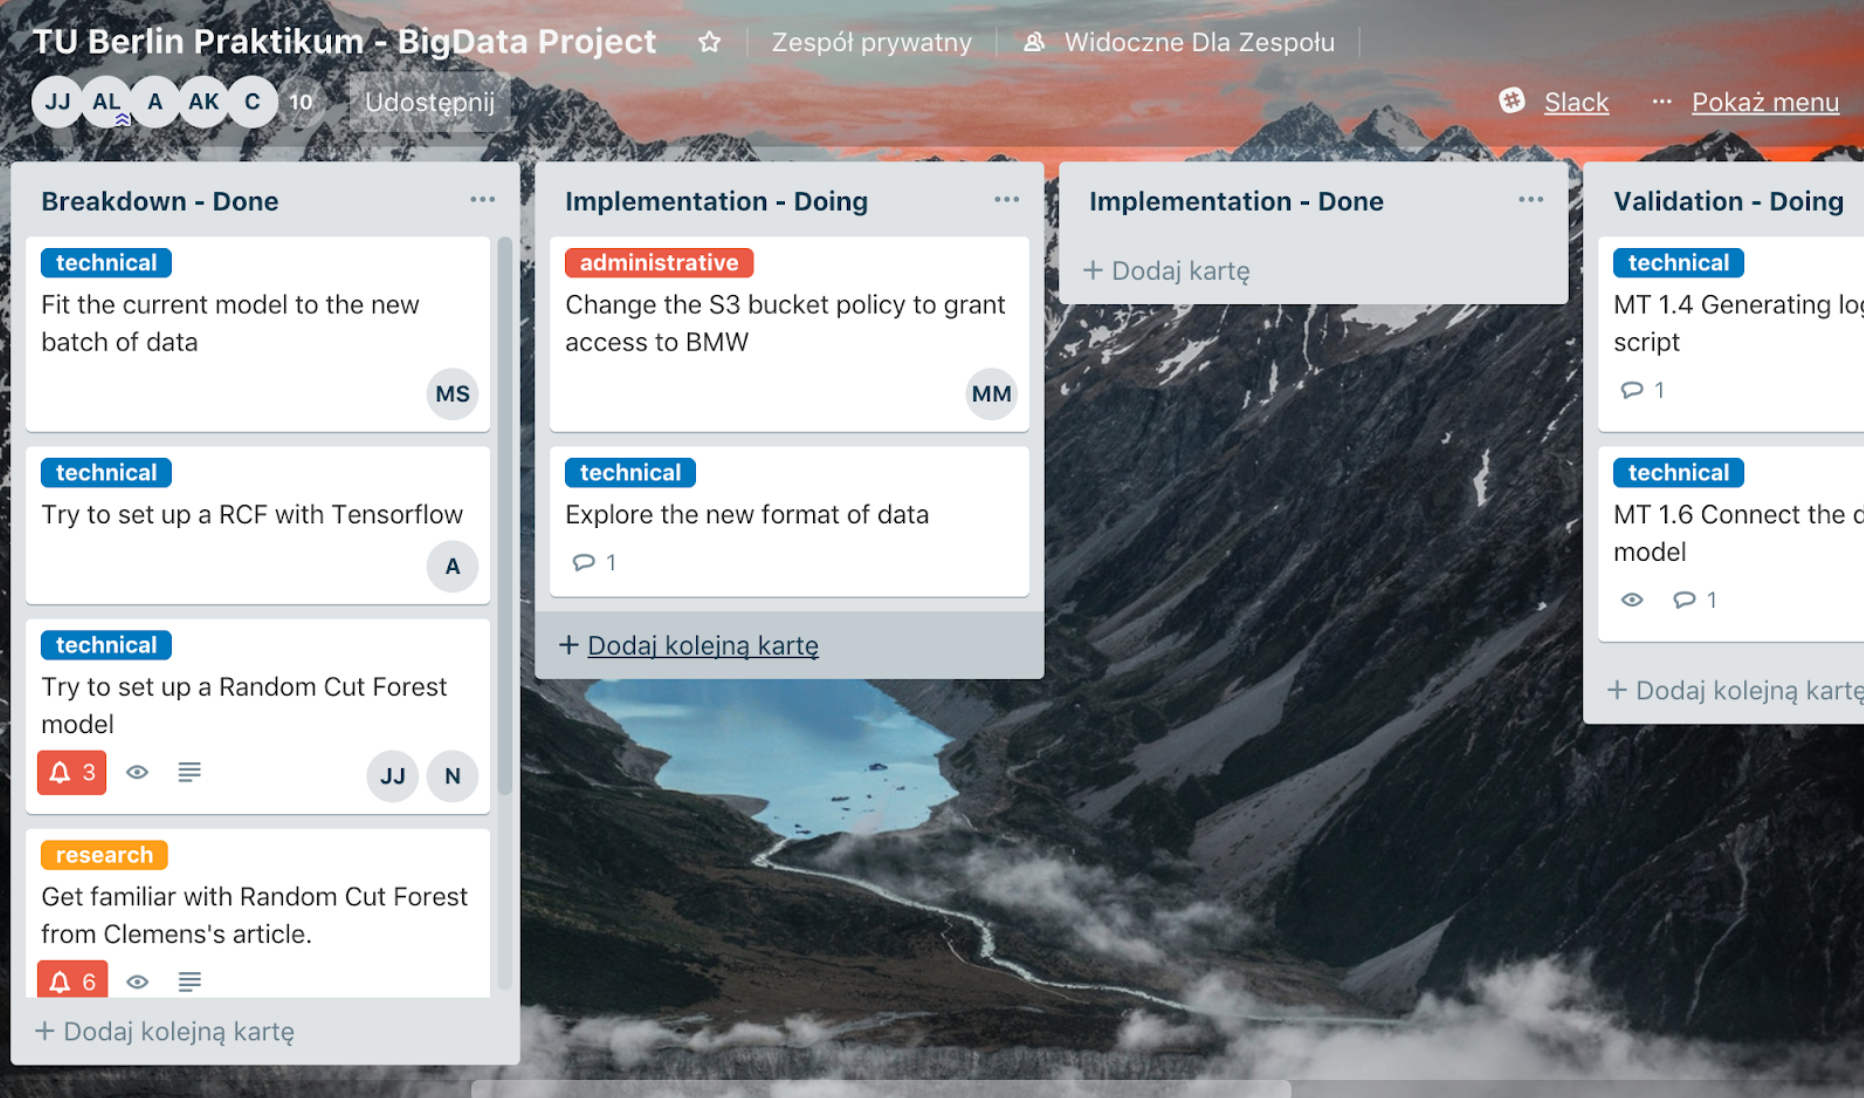
\includegraphics[width=1\textwidth]{images/trello.png}
        \caption{Big Data Analytics Trello board }
        \label{fig:trello_board_1}
    \end{figure}
    
After setting up the above mentioned columns, a user can start adding cards/user stories to the backlog. As seen in figure \ref{fig:trello_board_1}, Trello allows an user to add a title, a description (to detail the card), attachments, comments, due dates, responsible members and labels to a card.
It's worth noting, that for this project, the team used the board not just for programming related tasks. The Trello board was used for managing all project related assignments, for the purpose of registering each week's work.
\begin{figure}
    \centering
    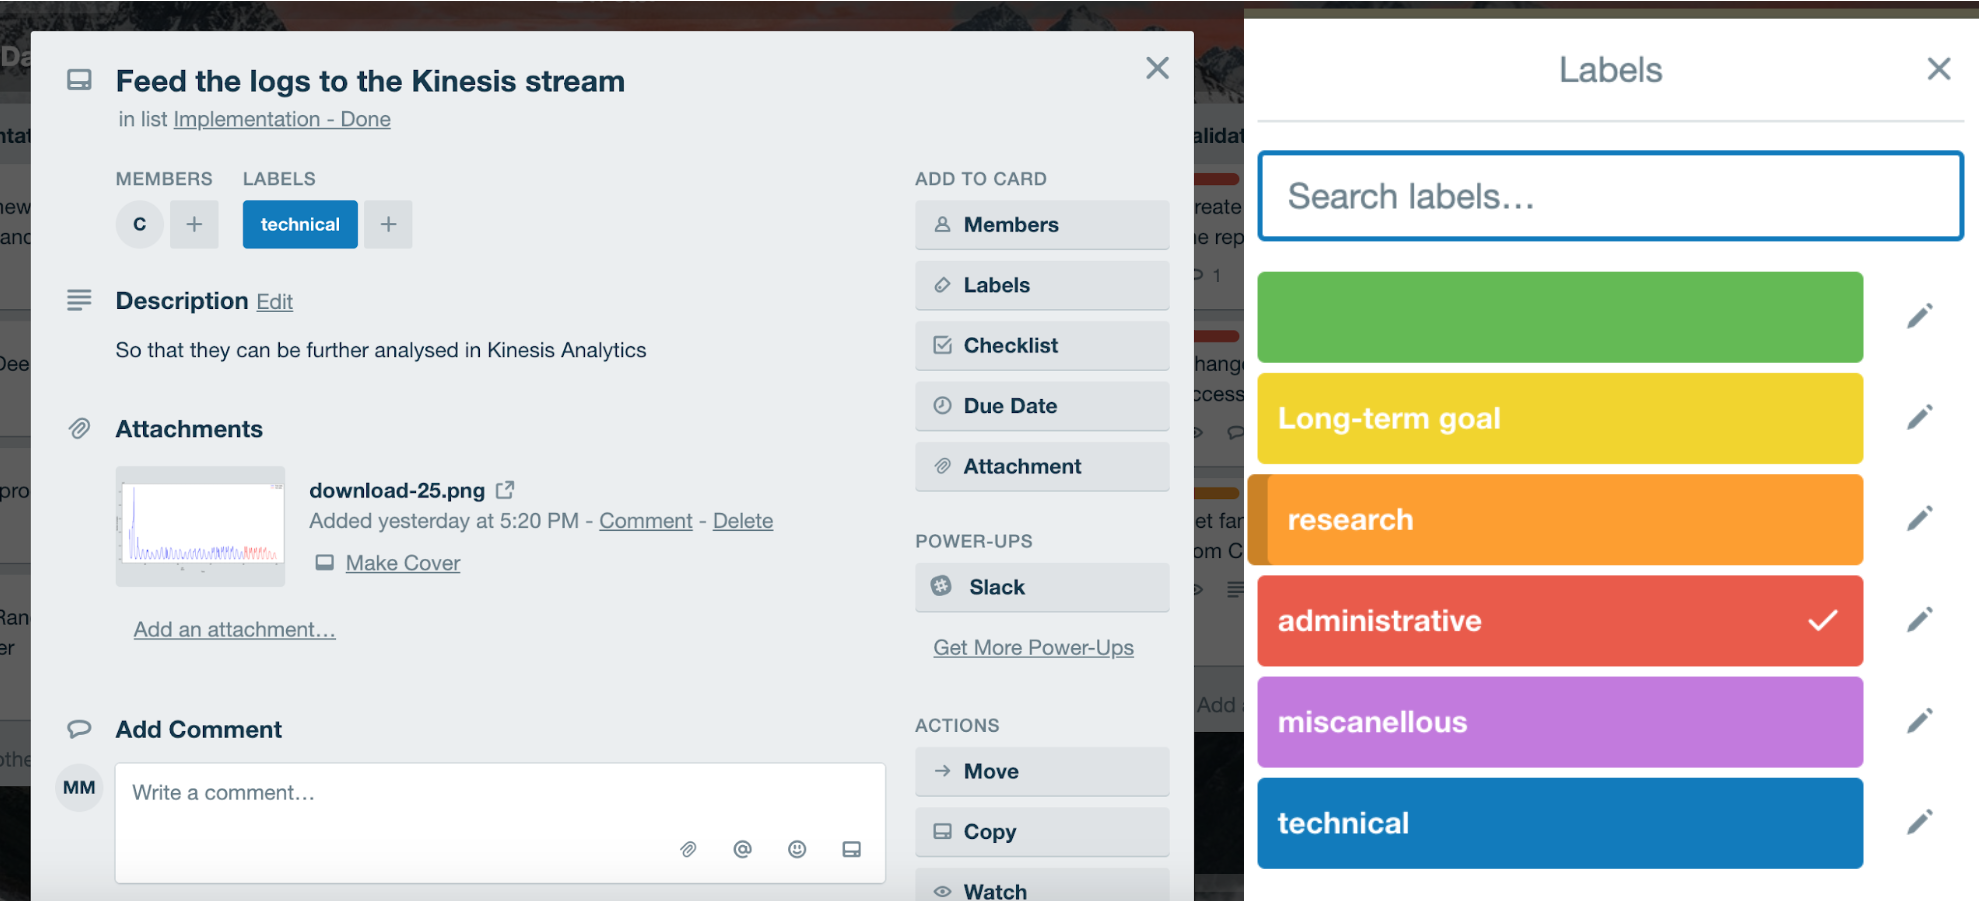
\includegraphics[width=1\textwidth]{images/card-view.png}
    \caption{Trello board card view with labeling details }
    \label{fig:trello_board_2}
\end{figure}
In this project, the team used the following series of labels to mark the purposes of the user-story (see \ref{fig:trello_board_2}):
    \begin{itemize}
    \item \textbf{Long-term goal}: indicates that the card is most likely a use case in the project, which should be broken down further into smaller tasks
    \item \textbf{Research}: marks tasks that require the team to look for papers, documentation, solutions to solve certain impediments
    \item \textbf{Administrative}: highlights that a task has a managerial character
    \item \textbf{Technical}: indicates a developer task;
    \item \textbf{Miscellaneous}: used for any other subjects that a task can have, except the ones mentioned above (e.g. creating the presentation or documentation paper)
\end{itemize}
    
    \section{Real time anomaly detection with Kinesis - Clemens}
\label{sec:real_time_anomaly_detection}
    \subsection{Motivation}
    This approach is inspired by a Medium blog post. 
    \footnote{\scriptsize{\url{https://medium.com/@devfire/real-time-anomaly-detection-in-vpc-flow-logs-part-1-introduction-55ed000e039b}}}
    The goal of the approach is to move the anomaly detection closer to a real-time setup. This means to continuously process the most recent data instead of analyzing data from the previous month or year to find anomalies. To give some more motivation about why this is actually an important issue, here is a quote from a job description from Netflix:
    \begin{displayquote}
        "Netflix Operational Insight Team is the team responsible for building common infrastructure to collect, transport, aggregate, process and visualize operational metrics. We build powerful systems to allow everyone at Netflix visibility into the state of our environment at both a macro and micro level."
    \end{displayquote}
    The fact that a leading and modern company like Netflix builds a whole team just dedicated to checking and visualizing the current system state in real time, underlines how important it is to know at every moment how your environment performs.\\
    AWS Kinesis is a very suitable tool for this problem for multiple reasons. First of all, Kinesis is designed to process streaming data. This means we can ingest real-time data which is a perfect fit for our given VPC flowlog data. Second Kinesis comes with Kinesis Data Analytics already built in. Amazon Kinesis Data Analytics offers easy ways to analyze streaming data, gain actionable insights, and respond to business needs in real time. In addition to that there is a SQL function called “Random cut forest with explanation” which is described by AWS as follows:
    \begin{displayquote}
        Computes an anomaly score and explains it for each record in your data stream. The anomaly score for a record indicates how different it is from the trends that have recently been observed for your stream. The function also returns an attribution score for each column in a record, based on how anomalous the data in that column is. For each record, the sum of the attribution scores of all columns is equal to the anomaly score. \cite{awsRcf}
    \end{displayquote}

    \subsection{Architecture}
    So with this prior knowledge let’s jump right into the system setup.
    First let’s get an overview of the system as it was implemented during the project phase:
    \begin{figure}
        \centering
        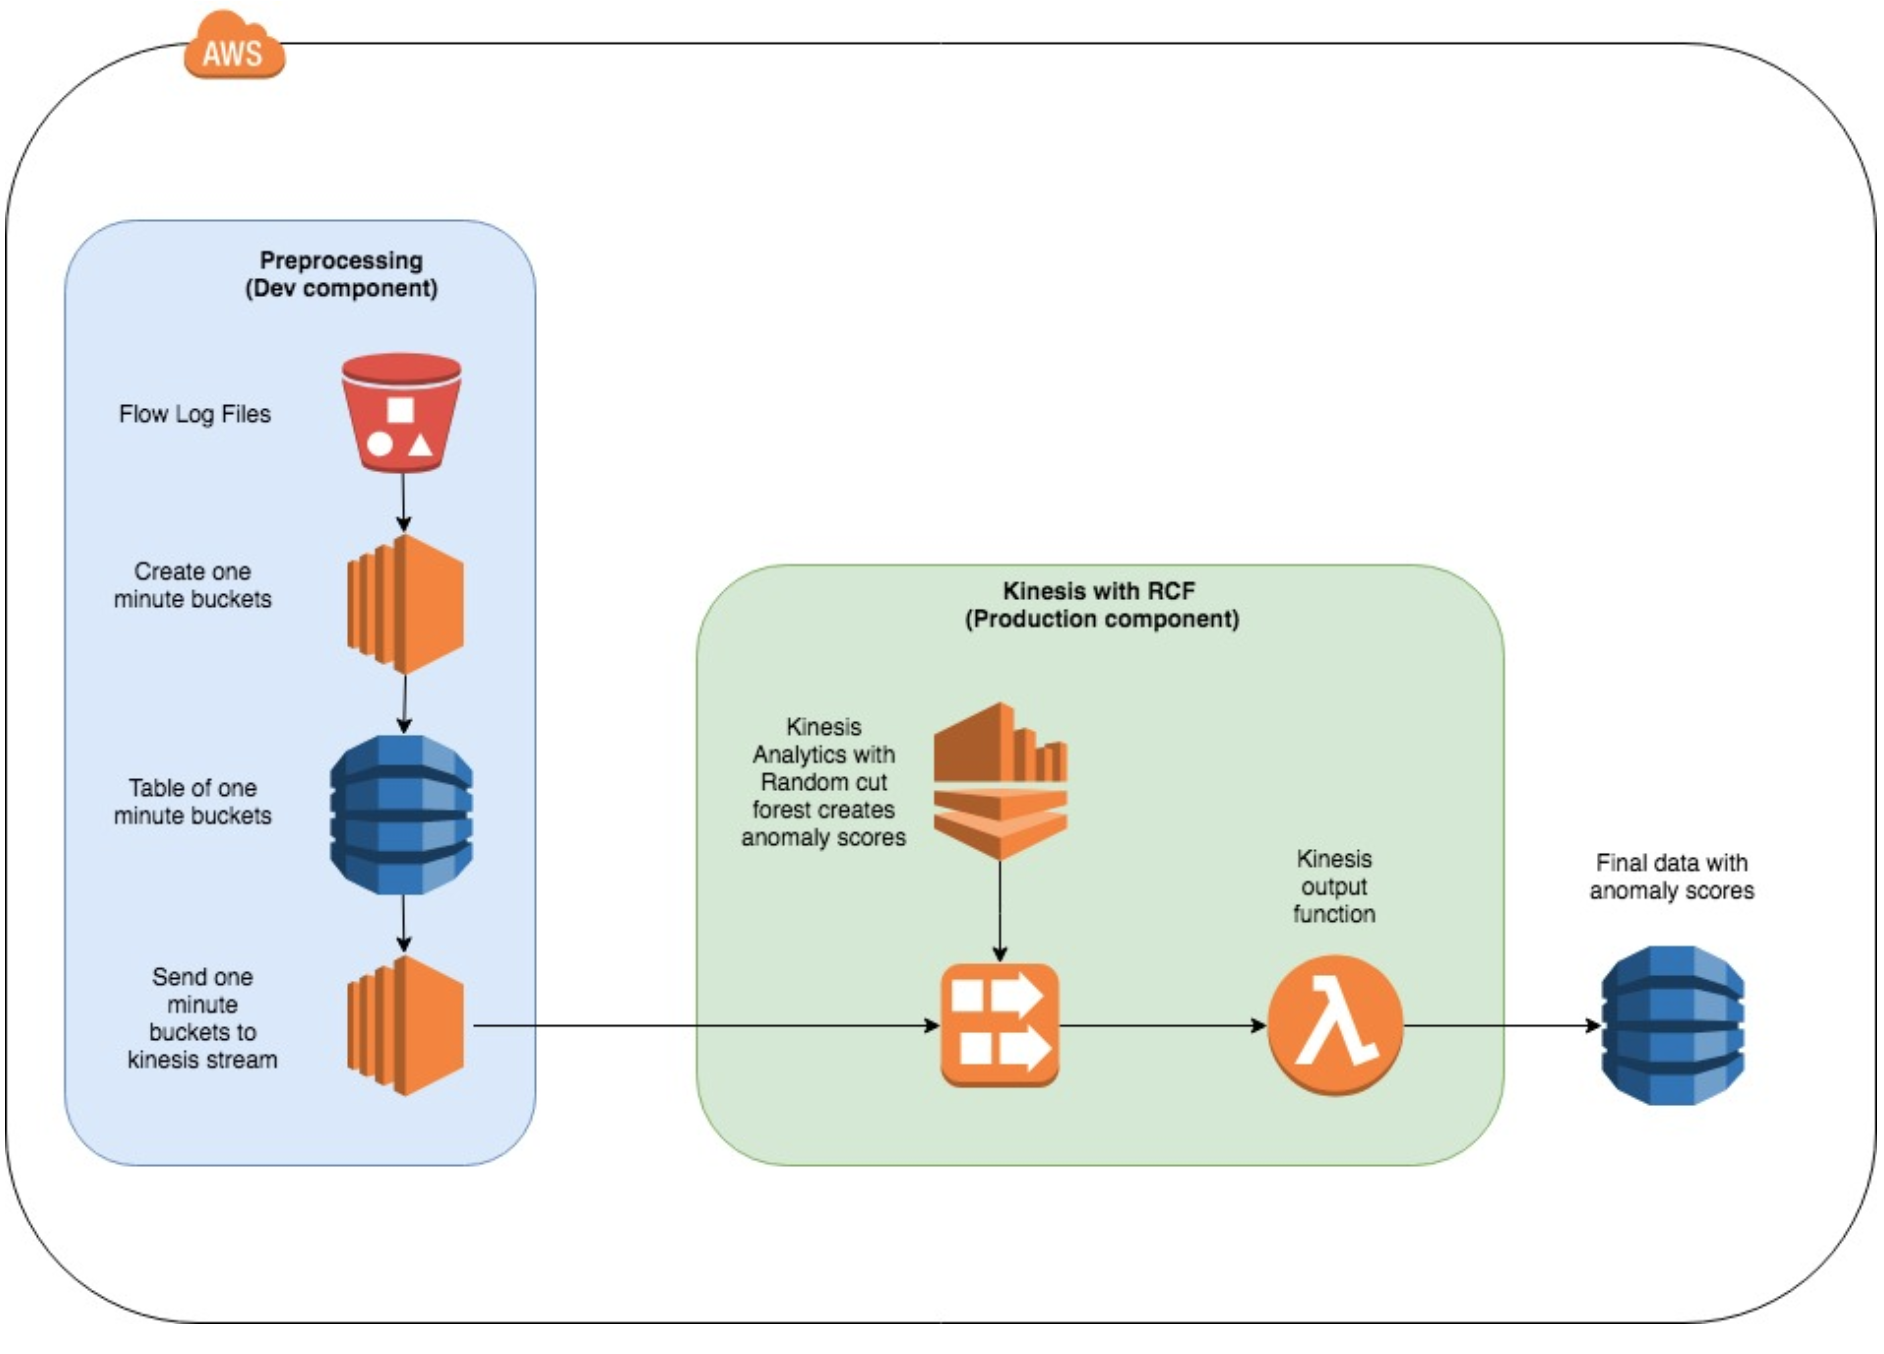
\includegraphics[width=1\textwidth]{images/medium-kinesis-setup.png}
        \caption{Medium Kinesis Random Cut Forest Setup}
        \label{fig:medium_kinesis_setup}
    \end{figure}
    \FloatBarrier
    First of all it should be noted that all the preprocessing components on the left (blue area in figure \ref{fig:medium_kinesis_setup}) would not be part of a production system. In a production system we would have a continuous stream of VPC flow logs which needs to be handled and preprocessed, whereas in the project setup we had all the flow logs data from the past in a S3 bucket. 
    
    \subsection{Preprocessing components (blue area in figure \ref{fig:medium_kinesis_setup})}
    In the following section we will look at the preprocessing setup in detail, keeping in mind that this is not created to run in production.
    
    \paragraph{S3: Flow Log Files}
    All the flow logs data provided by BMW lies in an S3 bucket called \textit{fog-bigdata-bmw-data}. As mentioned in \pageref{sec:fixed_data}, there are two types of data: first the metrics, which already contain summaries about how many requests were made to the system during a certain time interval. Another issue here was, that the time intervals are of different size (sometimes five minutes, sometimes four or six or something similar). Of course this is not a good basis to run our anomaly detection, because we cannot know what value we expect (since the size of the intervals are different). Therefore the second type of data is more suitable, namely the raw VPC Flowlogs. However, we want to look at how many requests are made to our system per minute and therefore we need to do some preprocessing.
    
    \paragraph{EC2: create one minute buckets}
    This is where the first script with the name \textit{createOneMinuteBuckets.py} comes in. This script is executed on an EC2 instance and reads all the flow log records from the S3 bucket. It creates one-minute buckets from the Flowlogs, so that we know for every one minute time interval how many requests were made to the system. 
    
    \paragraph{DynamoDB: table of one minute buckets}
    The information about these one minute buckets is then written into a DynamoDB table (called \verb|medium_bmw_data_to_kinesis|). For the sake of this project the data from the Kinesis table was then exported to a CSV file and the information about the weekdays was added (currently done in Excel). This means that for every one minute bucket we know the hour and the minute and also on which weekday it was recorded. This might be relevant because the expected number of request at 8am on a Sunday can be very different than 8am on a Monday, especially because the requests come from driving cars.  Of course this step will not be part of a production system (as mentioned before).
    
    \paragraph{EC2: send one minute buckets to Kinesis stream}
    The next script is called \textit{generateAnomalyScores.py}. The script and the final CSV file is uploaded to EC2 again. The script takes the data from this CSV file and sends it to the kinesis Stream called medium\textunderscore VPCFlowLogs. An alternative setup could be to read the data directly from DynamoDB and add the information about the weekday in the python script (instead of using CSV and Excel).\\
    This is where the preprocessing part (which would look different in a production system) ends and where the production component (green area in figure \ref{fig:medium_kinesis_setup}) comes into play.\\
    
    \subsection{Production component (green area in figure \ref{fig:medium_kinesis_setup})}
    In this section we assume that we already have all the data we need in the right format. This is the part of the system where the actual anomaly detection happens. This part of the the setup can be used in a production environment in the same or in a similar way. All the preprocessing is done and the data is already fed into the our Kinesis stream.
    \begin{figure}
        \centering
        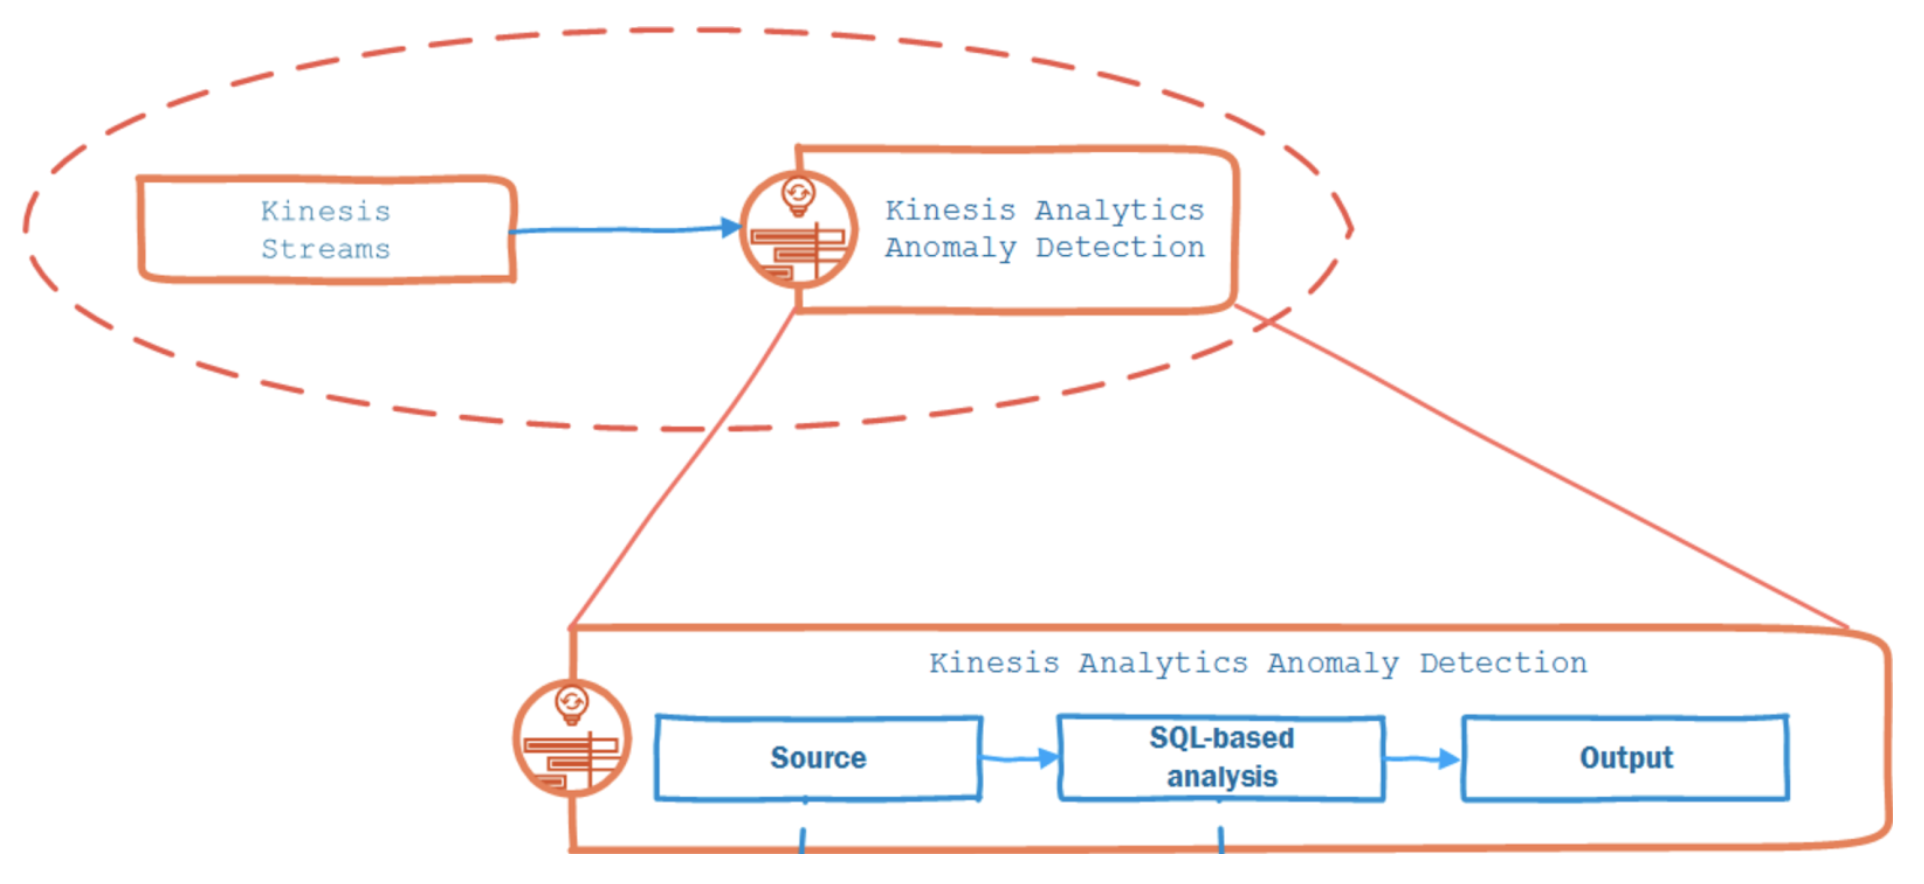
\includegraphics[width=1\textwidth]{images/kinesis-rcf.png}
        \captionsource{Kinesis Data Analytics with RCF}{\scriptsize{Source: https://medium.com/@devfire/real-time-anomaly-detection-in-vpc-flow-logs-part-5-anomaly-detection-d1fc9b61baf8}}
        \label{fig:medium_kinesis_data_analytics_rcf}
    \end{figure}
    \FloatBarrier
    The Kinesis stream has a Kinesis Data Analytics application which sends the data to random cut forest where the anomaly scores are created. This is the SQL code for the real time analytics:
    \begin{figure}
        \centering
        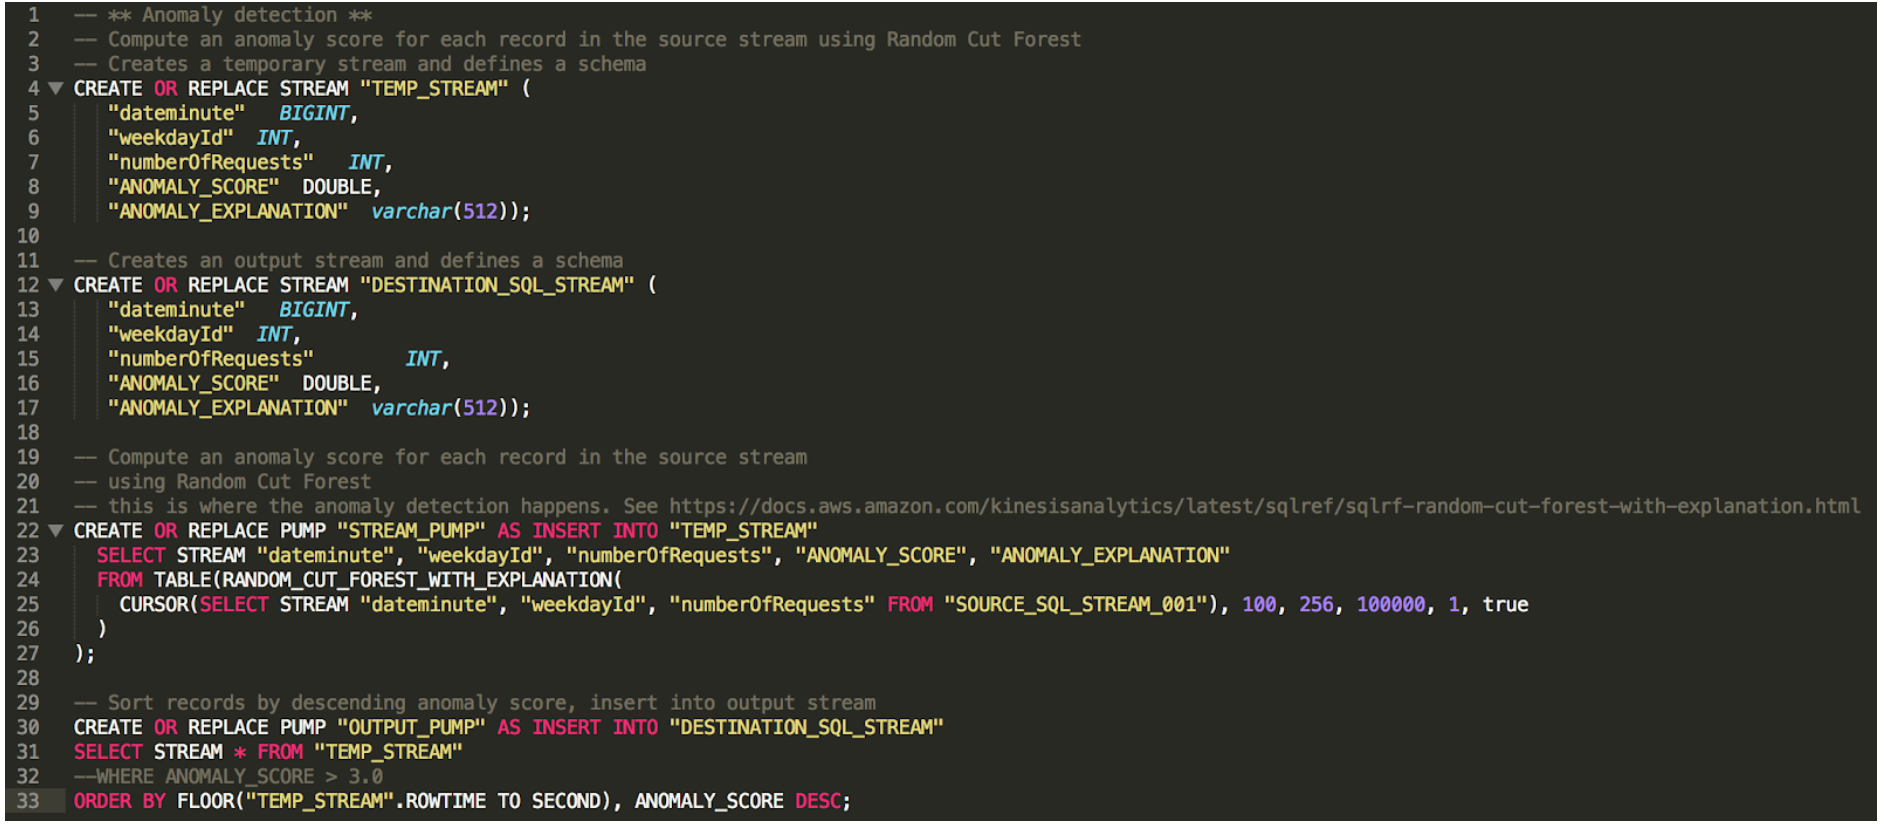
\includegraphics[width=1\textwidth]{images/sql-analytics.png}
        \captionsource{SQL code for real time analytics}{\\\scriptsize{Source: https://medium.com/@devfire/real-time-anomaly-detection-in-vpc-flow-logs-part-5-anomaly-detection-d1fc9b61baf8}}
        \label{fig:medium_sql_analytics}
    \end{figure}
    \FloatBarrier
    As we can see from the comment in line 32 it would be possible to already define a threshold here. This would then mean, that only anomaly scores which are higher than that specified threshold are sent to the output stream. However it is recommended to do implement this threshold in the output lambda function, to keep the threshold logic separate from the creation of the anomaly scores. Furthermore it is a lot easier to version and backup the lambda function in case the threshold is changed over time than to maintain different versions of the SQL code in the Kinesis Data Analytics part.
    \paragraph{Lambda: Kinesis output function}
    The output of the kinesis stream is sent to the Lambda function \verb|medium_bmw_kinesis_to_dynamodb_2|. \\
    This Lambda function just stores the results to another DynamoDB called \verb|kinesis_bmw_anomaly_scores|. Obviously this last database table was just for the purpose of the project phase to collect all the anomaly scores and visualize them in a graph but it is not needed in a production setup (as indicated in the system architecture). Instead in a production system this output function should contain the threshold for the anomaly score and then send a message or trigger a phone call if the threshold is exceeded.
    
    \subsection{Results}
    \begin{figure}[h]
        \centering
        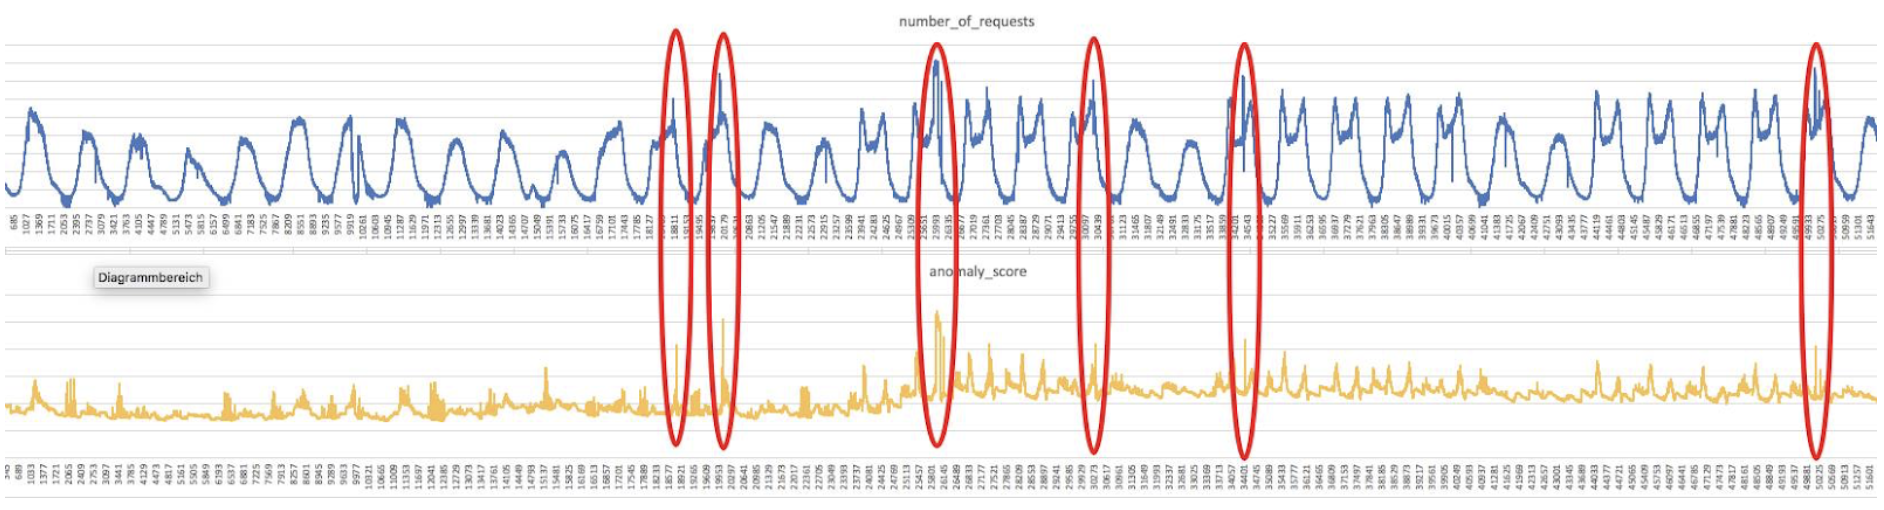
\includegraphics[width=1\textwidth]{images/kinesis-results.png}
        \caption{Visualisation of Kinesis Analytics Results}
        \label{fig:medium_kinesis_results}
    \end{figure}
    \FloatBarrier
    The blue graph at the top of figure \ref{fig:medium_kinesis_results} shows the requests to the the system per minute (from the one minute buckets). The orange graph at the bottom of figure \ref{fig:medium_kinesis_results} visualizes the anomaly score at that time. This means if we see an unexpected high peak or unexpected low drop in the first graph (number of requests per minute), in both cases we would expect a peak in the second graph (the anomaly scores). All in all this example does not show a perfect result (since we would expect our anomaly scores to be consistently low when there is no anomaly), however we have to take into account that this particular data set show the requests from December 21, 2018 until January 28, 2019 which means that it starts with the Christmas holidays which does not show the normal pattern of five weekdays followed by two weekends which we see towards the end.\\ Furthermore this is a series of 54,689 one minute buckets which is not a very long series to train on. Despite these factors of having limited and atypical data the high spikes in the anomaly scores (highlighted by the red ellipses) indicate that the approach in general is quite promising and that it can already detect anomalies.
    
    \subsection{Future work}
    The presented results are retrieved from feeding the data into the random cut forest in the following format: date-minute data, the weekday ID (as an integer) and number of requests.
    To refine the system further it might be interesting to try different combinations of these three input variables to see which combination gives the best results. This way it could be determined if it decreases the performance if we leave out the information about the weekday completely for example.
    
    \subsection{Implementation guide (Kinesis Random Cut Forest)} 
    This can be found in the appendix of this report (Appendix \ref{appendix-medium}) or online at \url{https://gist.github.com/clemenspeters/8e9025e3bd71e9087df154fb06f96328}
\chapter{Conclusions and Recommendations}
    Taking in consideration all the approaches mentioned throughout the paper for both prediction and anomaly detection models, and the fact that for BMW this is a more recent project, meaning that it does not possess a great amount of data to train and validate models, here are the project recommendations:
\begin{enumerate}
    \item Start the framework by implementing a \textit{Mean Predictor} algorithm for both anomaly detection and prediction. It trains well for small amount of data, takes less computational power, and will offer reliable results.
    \item Gather data for at least a year and save all the data in different granularity buckets. Plot and test the data and see what granularity offers best results compared to the computational power needed to process it. In terms of this project, 5 minutes granularity buckets proved to perform good, preserving all the anomalies while requiring less computational power to pre-process.
    \item Add a \textit{geolocation} component to the data and create different data pools for each regions of the globe, instead of smashing all information into one bucket. Such a change might give new insights into the gathered information. For example, it might reveal different holiday patterns for different countries, as well as take into consideration the specific holidays for different regions (christian celebration vs. muslim celebrations vs. asian holidays). 
    \item After having enough data, eventually even data that includes a location component too, run it through a \textit{DeepAR} model. As this algorithm allows the analysis of a couple of sources of data at the same time, try including other sources of data like weather or gas prices. This algorithm (for a significant amount of data) can find some dependencies between different sources of data and improve the predictions.
    \item In a year or two, implement a \textit{Random Cut Forest} model. After gathering some expert knowledge in handling anomalies, as well as information about the cause behind the anomalies and which deviations are worth looking into, you will have a better intuition about the right threshold. It might be an interesting idea to set a couple of threshold for different levels of anomalies, if this actually proves to bring any advantage in the way the anomalies are managed down the line.
    \item Run the data (after at least a year) through a \textit{Holt-Winters} model and try to identify seasonal trends (if they actually exist). Verify if the trends depend of the season/period of the year, some holidays or the geographical region. Such a model should offer new interesting insight into your data.
\end{enumerate}
%%=========================================
%Backmatter

\begin{appendices}
\include{backmatter/00_lessImportantText}
\include{backmatter/01_acronyms}
\include{backmatter/02_lexicon}
\include{backmatter/03_listings}
% Include more appendices as required.
\chapter{Real-time Anomaly Detection in VPC Flow Logs (in AWS)} \label{appendix-medium}

\section{Introduction}
Credit goes to Igor Kantor (\scriptsize{\url{https://medium.com/@devfire}}) who wrote the original post (5 parts) on Medium:

The goal of this GitHubGist is to support anyone who wants to implement the described architecture and get it running on AWS.
This means you should use both the Medium Post and this GitHubGist for the implementation (since I will not repeat all the text here).

On my aws account I used a prefix (medium) for all services, to easily find them amongst all the other running services/instance/funtions/roles etc. (just as a suggestion). It will make cleaning up your aws account easier later on.


In this GitHubGist we will focus on the anomaly detection ("components within the red dashes"):


\section{Part 1}
\scriptsize{\url{https://medium.com/@devfire/real-time-anomaly-detection-in-vpc-flow-logs-part-1-introduction-55ed000e039b}}

Just introduction text. Does not contain any code or implementation.


\section{Part 2}
\scriptsize{\url{https://medium.com/@devfire/real-time-anomaly-detection-in-vpc-flow-logs-part-2-proposed-architecture-32683755abf7}}

Gives an overview of the architecture.

In this GitHubGist we will focus on the anomaly detection ("components within the red dashes").


\section{Part 3}
\scriptsize{\url{https://medium.com/@devfire/real-time-anomaly-detection-in-vpc-flow-logs-part-3-kinesis-stream-1bdd8a9426f1}}

This is where the fun begins. 

Make sure you have the AWS Command Line Interface installed (\scriptsize{\url{https://docs.aws.amazon.com/de_de/cli/latest/userguide/cli-install-macos.html}}). 

If you just installed the aws cli, make sure you run \begin{lstlisting}[numbers=none]
aws configure
\end{lstlisting} 
to connect it to your aws account. 

Let's get started (with the article):

\begin{lstlisting}[numbers=none]
aws kinesis create-stream --stream-name "VPCFlowLogs" --shard-count 1\end{lstlisting}

\begin{lstlisting}[numbers=none]
vim allowCloudWatchAccesstoKinesis.json
\end{lstlisting}

Paste the content and substitute your region as needed (in line:  "Principal": { "Service": "logs.\textbf{us-east-1}.amazonaws.com" }, ).

Run the following command \textbf{from the same directory} where \textbf{allowCloudWatchAccesstoKinesis.json} is located:

\begin{lstlisting}[numbers=none]
aws iam create-role --role-name CloudWatchToKinesisRole --assume-role-policy-document file://./allowCloudWatchAccesstoKinesis.json
\end{lstlisting}

\begin{lstlisting}[numbers=none]
vim cloudWatchPermissions.json
\end{lstlisting}


Paste the content and \textbf{substitute the two resource arn strings} with yours.

Run the following command \textbf{from the same directory} where \textbf{cloudWatchPermissions.json} is located:

\begin{lstlisting}[numbers=none]
aws iam put-role-policy --role-name CloudWatchToKinesisRole --policy-name Permissions-Policy-For-CWL --policy-document file://./cloudWatchPermissions.json
\end{lstlisting}


\begin{lstlisting}[language=bash,numbers=left,stepnumber=1,breaklines=true]
aws logs put-subscription-filter \
    --log-group-name "VPCFlowLogs" \
    --filter-name "VPCFlowLogsAllFilter" \
    --filter-pattern "[version, account_id, interface_id, srcaddr != "-", dstaddr != "-", srcport != "-", dstport != "-", protocol, packets, bytes, start, end, action, log_status]" \
    --destination-arn "arn:aws:kinesis:us-east-1:31415926:stream/VPCFlowLogs" \
    --role-arn "arn:aws:iam::31415926:role/CloudWatchToKinesisRole"

\end{lstlisting}

\begin{lstlisting}[numbers=none]
brew install jq
\end{lstlisting}

\begin{lstlisting}[numbers=none]
aws kinesis get-records --limit 10 --shard-iterator $(aws kinesis get-shard-iterator --stream-name medium_VPCFlowLogs --shard-id shardId-000000000000 --shard-iterator-type TRIM_HORIZON | jq -r ."ShardIterator") | jq -r .Records[].Data | base64 -d | zcat
\end{lstlisting}

In my case 
\begin{lstlisting}[numbers=none]
aws kinesis get-records --limit 10 --shard-iterator $(aws kinesis get-shard-iterator --stream-name medium_VPCFlowLogs --shard-id shardId-000000000000 --shard-iterator-type TRIM_HORIZON | jq -r ."ShardIterator")
\end{lstlisting}
gives me the following:
\begin{lstlisting}[numbers=none, basicstyle=\tinysize]
{
    "Records": [],
    "NextShardIterator": "AAAAAAAAAAF3vrrgukNNTm4aHO8iRO5DXESr+ofQJFH57eXltrr1DTJW1DExKKckOxU5ZT2nFoQ2FOJsmfscXDRl9po0Q9Jb1Zvs9aytKcMLldmE6P7o/HZSC5uhlpT3/tFVAAMQAvqZ41MIFJqFik/kShb9q9oEB3WbYTrigihimcr1haixhIdQv2J6TJhJ6dZ1l6ggsVcnjbok1NZzIyzeABkS8fhLKSsJ/qIV+WmNigYX0MSYVA==",
    "MillisBehindLatest": 31385000
}
\end{lstlisting}

so when appending the 
\begin{lstlisting}[numbers=none]
| jq -r .Records[].Data | base64 -d | zcat
\end{lstlisting}
part to that command it gives me "no matches found: .Records[].Data". So I still have to figure out how to insert records here (probably just need to put traffic on the vpc).


\section{Part 4}
\scriptsize{\url{https://medium.com/@devfire/real-time-anomaly-detection-in-vpc-flow-logs-part-4-kinesis-analytics-c80cc4977e97}}


Navigate to the Kinesis Analytics page in the AWS console and click on Create Application.\\
\hspace*{1cm} Name it VPCFlowLogsAnalytics.\\
\hspace*{1cm} Hook it up to the VPCFlowLogs Kinesis stream you created earlier.\\
\hspace*{1cm} \textit{in case you can not create the application because you don't have enough\\
\hspace*{1cm} data see section \textbf{Amazon Kinesis Data Generator} on the bottom of this file.}\\
\hspace*{1cm} Enable Lambda pre-processing and say you want a new Lambda function. \\
\hspace*{2cm} Use blueprint \textbf{kinesis-analytics-process-compressed-record} for the lambda function\\
\hspace*{2cm} Name the lambda function \textit{KinesisAnalyticsProcessCompressedRecord}\\
\hspace*{2cm} Create in IAM a \textbf{lambda\textunderscore kinesis\textunderscore exec\textunderscore role} and give it AmazonKinesisFullAccess.\\
\hspace*{2cm} Assign  \textbf{lambda\textunderscore kinesis\textunderscore exec\textunderscore role} for your lambda function (\textit{KinesisAnalyticsProcessCompressedRecord}).\\
\hspace*{2cm} Increase the Timeout setting to at least 1 minute\\
\hspace*{1cm}Click on Discover Schema\\
\\
In my case the schema was not recognized and I had to manually create all the columns:


I had to rename the columns \textbf{start} and \textbf{end} (see error message in screenshot).
Here are the column names: 

\begin{lstlisting}[numbers=none]
version, account_id, interface_id, srcaddr, dstaddr, srcport, dstport, protocol, packets, bytes, start_, end_, action, log_status
\end{lstlisting}

I recommend to create them in reverse order (log\textunderscore status first, version last) so you dont have to sort manually.


\section{Part 5}
\scriptsize{\url{https://medium.com/@devfire/real-time-anomaly-detection-in-vpc-flow-logs-part-4-kinesis-analytics-c80cc4977e97}}

We are still where we left in part 4 (create Kinesis Analytics Application):

        Click on the blue \textbf{Go to SQL Editor} button.

\begin{lstlisting}[language=sql]
-- \textbf{ Anomaly detection \textbf{
-- Compute an anomaly score for each record in the source stream using Random Cut Forest
-- Creates a temporary stream and defines a schema
CREATE OR REPLACE STREAM "TEMP_STREAM" (
--   "APPROXIMATE_ARRIVAL_TIME"     timestamp,
--   "srcaddr"     varchar(16),
--   "dstaddr"   varchar(16),
   "bytes"        DOUBLE,
   "ANOMALY_SCORE"  DOUBLE,
   "ANOMALY_EXPLANATION"  varchar(512));
   
-- Creates an output stream and defines a schema
CREATE OR REPLACE STREAM "DESTINATION_SQL_STREAM" (
--   "APPROXIMATE_ARRIVAL_TIME"     timestamp,
 --  "srcaddr"     varchar(16),
--   "dstaddr"   varchar(16),
   "bytes"        DOUBLE,
   "ANOMALY_SCORE"  DOUBLE,
   "ANOMALY_EXPLANATION"  varchar(512));
 
-- Compute an anomaly score for each record in the source stream
-- using Random Cut Forest
CREATE OR REPLACE PUMP "STREAM_PUMP" AS INSERT INTO "TEMP_STREAM"
--  SELECT STREAM "APPROXIMATE_ARRIVAL_TIME", "srcaddr", "dstaddr", "bytes", "ANOMALY_SCORE", "ANOMALY_EXPLANATION"
-- SELECT STREAM "srcaddr", "dstaddr", "bytes", "ANOMALY_SCORE", "ANOMALY_EXPLANATION"
  SELECT STREAM "bytes", "ANOMALY_SCORE", "ANOMALY_EXPLANATION" 
  FROM TABLE(RANDOM_CUT_FOREST_WITH_EXPLANATION(
    CURSOR(SELECT STREAM "bytes" FROM "SOURCE_SQL_STREAM_001"), 100, 256, 100000, 1, true
  )
);
-- Sort records by descending anomaly score, insert into output stream
CREATE OR REPLACE PUMP "OUTPUT_PUMP" AS INSERT INTO "DESTINATION_SQL_STREAM"
SELECT STREAM * FROM "TEMP_STREAM"
--WHERE ANOMALY_SCORE > 3.0
ORDER BY FLOOR("TEMP_STREAM".ROWTIME TO SECOND), ANOMALY_SCORE DESC;
\end{lstlisting}

(It is mentioned that credits go to Curtis Mitchell: \scriptsize{\url{https://medium.com/@curtis_mitchell}})

To understand where the anomaly detection happens see:\\ \scriptsize{\url{https://docs.aws.amazon.com/kinesisanalytics/latest/sqlref/sqlrf-random-cut-forest-with-explanation.html}}

\textbf{The following part is not from the Medium article, but was added for clarification}


\section{Part 5 continued}

Create new lambda function using the blueprint \textbf{kinesis-analytics-output}

Name the lambda function \textbf{kinesis\textunderscore analytics\textunderscore destination}

Open your \textit{VPCFlowLogsAnalytics} in \textit{Kinesis Analytics applications}

Click \textbf{Connect new destination} button

Choose \textit{AWS Lambda function} as destination and select \textbf{kinesis\textunderscore analytics\textunderscore destination}

As \textit{In-application stream name} choose \textbf{DESTINATION\textunderscore SQL\textunderscore STREAM}

Click \textbf{Save and continue}

\section{Amazon Kinesis Data Generator (used for part 4)}
To supply the Kinesis Stream with data I had to set up an \textbf{Amazon Kinesis Data Generator} first.

Open the page \scriptsize{\url{https://awslabs.github.io/amazon-kinesis-data-generator/web/help.html.}}

Download the CloudFormation template \scriptsize{\url{https://s3-us-west-2.amazonaws.com/kinesis-helpers/cognito-setup.json}}


Click the blue \textbf{Create a Cognito User with CloudFormation} button (on the \scriptsize{\url{https://awslabs.github.io/amazon-kinesis-data-generator/web/help.html}}).

You are redirected to aws console. 

Choose \textbf{Upload a template to Amazon S3} and choose the \textbf{cognito-setup.json} which you downloaded before.

Click the \textbf{next} button (bottom right).

Read the rest of the \scriptsize{\url{https://awslabs.github.io/amazon-kinesis-data-generator/web/help.html}} to learn how to access and use the Amazon Kinesis Data Generator.

\section{allowCloudWatchAccesstoKinesis.json}
\begin{lstlisting}[language=json]
{
  "Statement": {
    "Effect": "Allow",
    "Principal": { "Service": "logs.us-east-1.amazonaws.com" },
    "Action": "sts:AssumeRole"
  }
}
\end{lstlisting}

\section{cloudWatchPermissions.json}
\begin{lstlisting}[language=json]
{
  "Statement": [
    {
      "Effect": "Allow",
      "Action": "kinesis:PutRecord",
      "Resource": "arn:aws:kinesis:us-east-1:31415926:stream/VPCFlowLogs"
    },
    {
      "Effect": "Allow",
      "Action": "iam:PassRole",
      "Resource": "arn:aws:iam::31415926:role/CloudWatchToKinesisRole"
    }
  ]
}
\end{lstlisting}
\end{appendices}


\cleardoublepage
\addcontentsline{toc}{chapter}{Bibliography}
\defbibheading{notonline}{\chapter*{Bibliography}}
\printbibliography[heading=notonline, nottype=online]
\defbibheading{online}{\chapter*{Bibliography (Online)}}
\printbibliography[heading=online, type=online]
%%=============================================

\end{document}